\documentclass{article}
\usepackage{notes}


\title{Teoria di Data Intensive}
\author{}
\date{}



\begin{document}

\maketitle
\tableofcontents


\section{Richiami di Algebra Lineare}

L'algebra lineare studia vettori, matrici, spazi vettoriali, sistemi di equazioni lineari e trasformazioni lineari.


\paragraph{Vettori} Un vettore è una tupla di $n$ numeri (componenti) reali, ad esempio, $v = (v_1, \dots, v_n)$. Esempio: $(12, 4.5, 2.1)$.
Geometricamente, le componenti di un vettore sono le coordinate di un punto in uno spazio N-dimensionale.
\begin{itemize}
    \item La direzione di $v$ è data dalla retta passante per gli estremi, il verso dall'orientamento della freccia.
    \item Il vettore nullo ha tutte le componenti uguali a 0.
    \item Il modulo di $v$ è la sua lunghezza; un vettore unitario ha modulo 1.
\end{itemize}

\begin{figure}[H] 
    \centering
    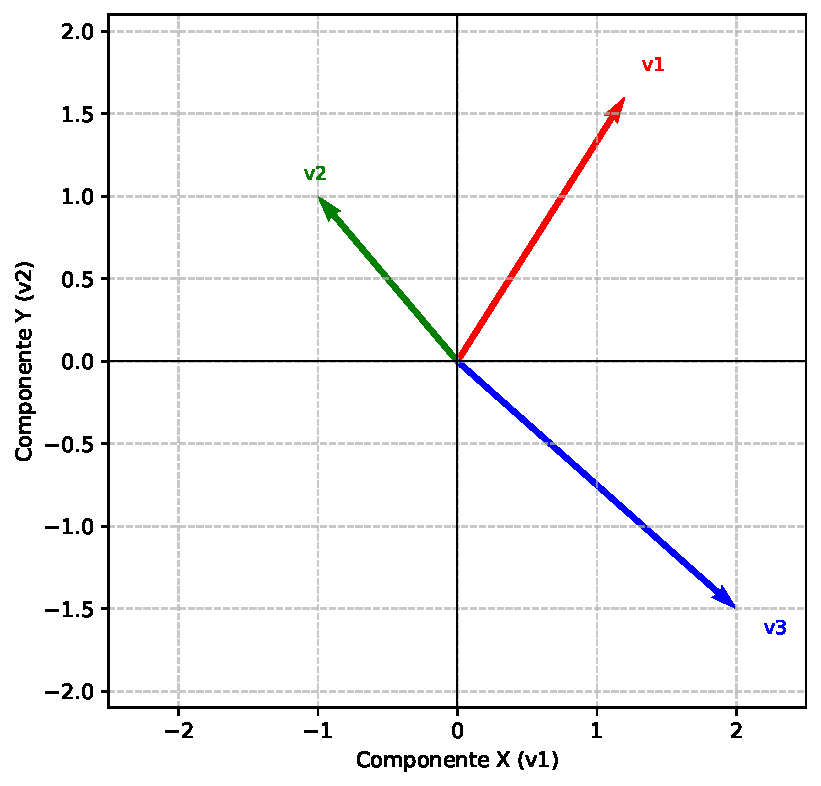
\includegraphics[width=0.6\textwidth]{images/vector_example.pdf}
    \caption{Esempi di vettori a 2 valori in un piano 2D con origine in (0,0).}
    \label{fig:vector_example}
\end{figure}

\begin{definitionbox}{Somma di Vettori}
    La somma di due vettori di pari dimensioni è data dal vettore con le componenti sommate una ad una.
    Esempio: $(1.2, 1.6) + (-1, 1) = (1.2-1, 1.6+1) = (0.2, 2.6)$.
\end{definitionbox}

\begin{definitionbox}{Prodotto tra Scalare e Vettore}
    Il prodotto tra uno scalare $x$ (un numero singolo) ed un vettore è dato dal vettore con le componenti moltiplicate per $x$.
    Esempio: $2 \cdot (1, -0.8) = (2 \cdot 1, -2 \cdot 0.8) = (2, -1.6)$.
    Anche: $-1 \cdot (1, -0.8) = (-1, 0.8)$.
\end{definitionbox}

\begin{figure}[H]
    \centering
    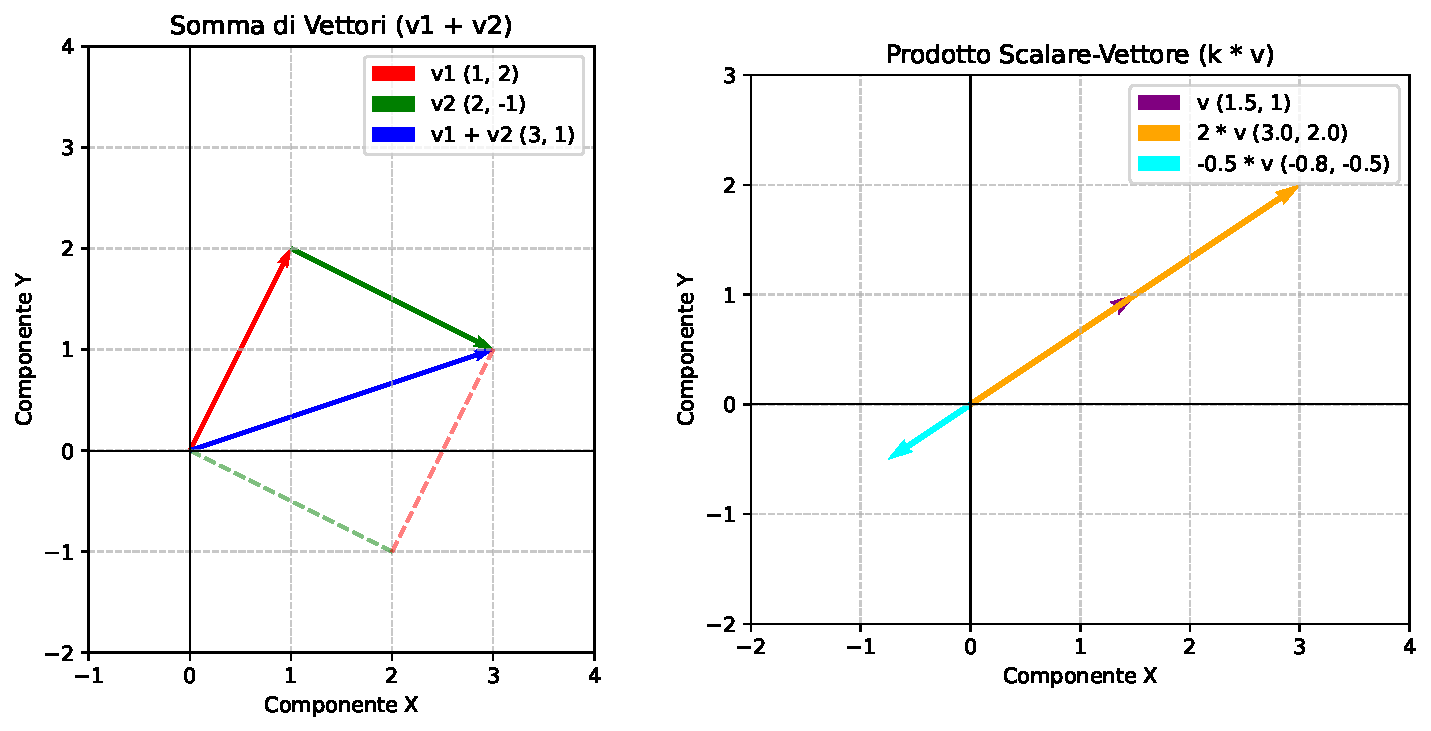
\includegraphics[width=1\textwidth]{images/vector_operations_example.pdf}
    \caption{Visualizzazione della somma di vettori e del prodotto scalare-vettore.}
    \label{fig:vector_ops_example}
\end{figure}


\paragraph{Norma Euclidea} La norma euclidea di un vettore $a$ (detta anche norma 2) è la radice quadrata della somma dei quadrati delle sue componenti.
Formula: $||a|| = \sqrt{\sum_{i=1}^{n} a_i^2}$.
Esempio: sia $a = (2.5, 2.8)$, allora $||a|| = \sqrt{2.5^2 + 2.8^2} \approx 3.7$.
La norma 2 è la lunghezza di $a$ ed equivale ad applicare il teorema di Pitagora alle componenti.
Dividendo un vettore $a$ per la sua norma $||a||$, si ottiene il vettore unitario di $a$, che ha norma 1: $\frac{a}{||a||}$. Esempio con $a=(2.5, 2.8)$: $\frac{a}{||a||} \approx (0.67, 0.75)$.

\paragraph{Prodotto Scalare tra due Vettori} Il prodotto scalare (dot product) tra due vettori $a, b$ di dimensioni $n$ è la somma dei prodotti delle rispettive coppie di componenti.
Formula: $a \cdot b = \sum_{i=1}^{n} a_i \cdot b_i$.
Esempio: $a = (-1.2, 4.5)$, $b = (2.5, 2.8)$, allora $a \cdot b = -1.2 \times 2.5 + 4.5 \times 2.8 = -3 + 12.6 = 9.6$.

Geometricamente, $a \cdot b$ è un indicatore della lunghezza della proiezione ortogonale di $a$ su $b$.
Più precisamente, $a \cdot b = ||a|| \cdot ||b|| \cdot \cos(\theta)$, dove $\theta$ è l'angolo tra i due vettori. Questo implica che $a \cdot b = ||b|| \cdot (||a|| \cos(\theta))$, dove $||a|| \cos(\theta)$ è la lunghezza della proiezione ortogonale di $a$ su $b$.
Quindi, il prodotto scalare è la proiezione ortogonale di $a$ su $b$, scalata rispetto alla lunghezza di $b$.
Un prodotto scalare maggiore indica una maggiore similarità (minore angolo) tra i due vettori. Se $\cos(\theta) = 0$ (angolo di $90^\circ$), i vettori sono ortogonali e il loro prodotto scalare è 0. Se $\cos(\theta) = 1$ (angolo di $0^\circ$), i vettori hanno la stessa direzione e il prodotto scalare è massimizzato.

\paragraph{Matrici} Una matrice $m \times n$ è una tabella di numeri reali con $m$ righe e $n$ colonne.
Esempio: $A_{2,3} = \begin{pmatrix} a_{1,1} & a_{1,2} & a_{1,3} \\ a_{2,1} & a_{2,2} & a_{2,3} \end{pmatrix}$, come $\begin{pmatrix} 2.1 & -4 & 2.4 \\ -3.2 & 1.1 & 5 \end{pmatrix}$.
\begin{itemize}
    \item Ogni riga ed ogni colonna è rappresentabile come un vettore.
    \item Una matrice con una sola riga ($1 \times n$) o una sola colonna ($m \times 1$) è detta rispettivamente matrice riga o matrice colonna.
    \item Una matrice è nulla se tutti gli elementi sono 0.
\end{itemize}

\paragraph{Operazioni Elementari su Matrici} La somma tra matrici di pari dimensioni avviene sommando gli elementi corrispondenti, come per i vettori (operazione element-wise).
Il prodotto tra uno scalare e una matrice avviene moltiplicando ogni elemento della matrice per lo scalare, come per i vettori (operazione element-wise).


\begin{definitionbox}{Prodotto tra Matrici}
    Il prodotto tra due matrici $A_{m,p}$ e $B_{p,n}$ è una matrice $C_{m,n}$ dove la cella $c_{i,j}$ è data dal prodotto scalare tra il vettore riga $i$ di $A$ e il vettore colonna $j$ di $B$.
    Formula: $(AB)_{i,j} = \sum_{k=1}^{p} a_{i,k} \cdot b_{k,j}$.
    Nota: Il numero di colonne di A deve essere uguale al numero di righe di B. Il prodotto tra matrici generalmente non è commutativo ($AB \neq BA$).
\end{definitionbox}

\paragraph{Matrice Trasposta} Data una matrice $A_{m \times n}$, la sua trasposta $A^T$ è la matrice $n \times m$ in cui righe e colonne sono scambiate.
Proprietà:
\begin{itemize}
    \item $(AB)^T = B^T A^T$
    \item $(A+B)^T = A^T + B^T$
\end{itemize}

\paragraph{Matrici Quadrate} Una matrice si dice quadrata se ha tante righe quante colonne ($m=n$). Il numero di righe (o colonne) è detto ordine della matrice.
Una matrice quadrata $A$ è:
\begin{itemize}
    \item Simmetrica se $A = A^T$.
    \item Antisimmetrica se $A = -A^T$.
\end{itemize}

\paragraph{Matrici Diagonali} La diagonale principale di una matrice quadrata è il vettore degli elementi $a_{i,i}$ (da $a_{1,1}$ a $a_{n,n}$).
Una matrice quadrata è diagonale se tutti gli elementi al di fuori della diagonale principale sono 0.

\paragraph{Matrice Identità} La matrice identità di ordine $n$, indicata con $I_n$, è la matrice diagonale $n \times n$ con tutti gli elementi della diagonale principale pari a 1.
Esempio: $I_3 = \begin{pmatrix} 1 & 0 & 0 \\ 0 & 1 & 0 \\ 0 & 0 & 1 \end{pmatrix}$.
La matrice identità è l'elemento neutro della moltiplicazione tra matrici: $I_m A = A I_n = A$ per qualsiasi matrice $A_{m \times n}$.

\paragraph{Matrice Inversa} Una matrice quadrata $A_{n \times n}$ è invertibile se esiste una matrice inversa $A^{-1}$ di pari dimensioni tale che $A A^{-1} = A^{-1} A = I_n$.
Una matrice quadrata non invertibile è detta singolare.
Proprietà per matrici invertibili:
\begin{itemize}
    \item $(AB)^{-1} = B^{-1} A^{-1}$
    \item $(A^{-1})^T = (A^T)^{-1}$
\end{itemize}

\subsection{Sistemi di Equazioni Lineari in Forma di Matrici}
Un sistema di $m$ equazioni lineari in $n$ incognite può essere scritto in forma matriciale come $Ax = b$.
Qui, $A$ è la matrice dei coefficienti ($m \times n$), $x$ è il vettore colonna delle incognite ($n \times 1$), e $b$ è il vettore colonna dei termini noti ($m \times 1$).
Se la matrice $A$ è quadrata ($m=n$) e invertibile, il vettore delle incognite $x$ può essere trovato come: $x = A^{-1}b$.

\begin{examplebox}{Risoluzione di Sistemi Lineari}
    Quesito: In un totale di 7 monete da 5 e 10 centesimi il cui valore è 55 centesimi, quante sono le monete dei due tagli?
    Sia $x_1$ il numero di monete da 5 centesimi e $x_2$ il numero di monete da 10 centesimi.
    Il sistema di equazioni è:
    $$ \begin{cases} x_1 + x_2 = 7 \\ 5x_1 + 10x_2 = 55 \end{cases} $$
    In forma matriciale $Ax=b$:
    $$ \begin{pmatrix} 1 & 1 \\ 5 & 10 \end{pmatrix} \begin{pmatrix} x_1 \\ x_2 \end{pmatrix} = \begin{pmatrix} 7 \\ 55 \end{pmatrix} $$
    La soluzione è $x_1=3$ (monete da 5c) e $x_2=4$ (monete da 10c).
\end{examplebox}


\subsection{Perché Vettori e Matrici nel Machine Learning e Data Science?}
L'algebra lineare, con il suo focus su vettori e matrici, è cruciale nel campo del machine learning, della data science e del deep learning perché i dati del mondo reale vengono tipicamente modellati e rappresentati utilizzando queste strutture matematiche. Questa rappresentazione permette di applicare in modo efficiente algoritmi complessi per analizzare i dati, identificare pattern e fare previsioni.

Ecco alcuni esempi pratici di come i dati vengono modellati:

\begin{itemize}
    \item \textbf{Dati Utente-Prodotto (Sistemi di Raccomandazione):}
          Le interazioni tra utenti e prodotti (come acquisti o recensioni) possono essere rappresentate da una matrice. In questa matrice:
          \begin{itemize}
              \item Ogni riga può essere un vettore che rappresenta un singolo utente.
              \item Le componenti di questo vettore indicano i prodotti che l'utente ha acquistato o recensito. Ad esempio, un valore positivo potrebbe indicare un acquisto, mentre uno zero indica nessuna interazione.
          \end{itemize}

    \item \textbf{Rappresentazione di Oggetti e Fenomeni Complessi:}
          Entità del mondo reale come automobili, abitazioni, immagini, o anche testi, vengono trasformate in vettori di caratteristiche (features) per poter essere elaborate dagli algoritmi di machine learning.
          \begin{itemize}
              \item \textbf{Automobili:} Ogni automobile può essere rappresentata da un vettore le cui componenti sono le sue caratteristiche, come costi di manutenzione passati, costi di assicurazione, costi di proprietà (bollo), costi totali di rifornimento, ecc.. Una variabile di interesse da predire potrebbe essere, ad esempio, i "costi di manutenzione dell'anno al tempo t+1".
              \item \textbf{Abitazioni:} Analogamente, ogni abitazione può essere descritta da un vettore con caratteristiche quali metri quadri, vetustà, quartiere di ubicazione, numero di stanze, numero di bagni, piano, ecc.. L'obiettivo di un modello di machine learning potrebbe essere quello di predire il "prezzo di vendita" dell'abitazione.
          \end{itemize}
\end{itemize}

In sostanza, la capacità di rappresentare dati eterogenei in un formato numerico strutturato come vettori e matrici è un passaggio fondamentale. Questa trasformazione permette agli algoritmi di machine learning di elaborare i dati, "apprendere" da essi e generare output utili come classificazioni, regressioni o raccomandazioni.



\section{Applicazioni Predittive con Regressione Lineare}


\subsection{Introduzione al Machine Learning}
Il Machine Learning (ML) fornisce metodi generali per estrarre modelli di conoscenza da insiemi di dati. L'obiettivo è scoprire una funzione che associ ad ogni dato di input una classe o un valore numerico. Questo è applicabile a qualsiasi problema in cui esistano dati sufficienti.
Esempi di applicazioni includono:
\begin{itemize}
    \item Classificare clienti, recensioni o immagini mediche.
    \item Predire propensioni di acquisto, l'andamento delle vendite, il consumo energetico o il valore di titoli di borsa.
\end{itemize}

\begin{notebox}{Tipi di Apprendimento nel Machine Learning}
    Il Machine Learning si può categorizzare in base a:
    \begin{itemize}
        \item \textbf{Tipo di variabile di output da predire}:
              \begin{itemize}
                  \item \textit{Variabili discrete}: Ad esempio, classificare i clienti in "fedeli" e "non fedeli".
                  \item \textit{Variabili continue}: Ad esempio, predire l'andamento dei consumi energetici o delle vendite di un prodotto.
              \end{itemize}
        \item \textbf{Tipo di variabili in input per il training}:
              \begin{itemize}
                  \item \textit{Variabili strutturate}: Dati tabellari con domini noti per ogni attributo (es. classificare clienti in base agli acquisti).
                  \item \textit{Variabili destrutturate}: Testi come frasi, documenti, email (es. classificare email spam/non spam).
              \end{itemize}
        \item \textbf{Tipo di algoritmi di learning}:
              \begin{itemize}
                  \item \textit{Supervisionati}: I dati di training sono preclassificati o hanno un output noto.
                  \item \textit{Non supervisionati}: I dati non sono preclassificati (es. clustering).
              \end{itemize}
    \end{itemize}
\end{notebox}

\begin{examplebox}{Processo di Estrazione della Conoscenza (Learning Supervisionato) }
    Il processo generale per sistemi di IA basati sul learning supervisionato include le seguenti fasi:
    \begin{enumerate}
        \item Raccolta dei dati, analisi esplorativa e della qualità.
        \item Trattamento di valori mancanti, normalizzazione, standardizzazione.
        \item Selezione di \textit{feature} (variabili rilevanti).
        \item Divisione dei dati in \textit{training set}, \textit{validation set} e \textit{test set}.
        \item Estrazione di modelli di conoscenza dal training set con algoritmi di ML, individuando i parametri che massimizzano l'accuratezza sul validation set.
        \item Il test set misura l'accuratezza del modello su dati nuovi/ignoti.
        \item Interpretazione dei migliori modelli estratti.
        \item Deployment della conoscenza in applicazioni.
    \end{enumerate}
\end{examplebox}

\subsection{Regressione Lineare: Predire Variabili Continue}
La regressione lineare è una tecnica statistica che stima, a partire da un dataset, una funzione lineare che associa variabili di input (variabili indipendenti o \textit{features}) ad una variabile di output continua (variabile dipendente).
\begin{itemize}
    \item Con una sola variabile indipendente, si parla di \textbf{regressione lineare univariata}.
    \item Con più variabili indipendenti, si ha la \textbf{regressione lineare multivariata}.
\end{itemize}
Esistono diversi metodi di regressione che possono estrarre funzioni con andamenti diversi (polinomiali, logaritmiche, ecc.). In ogni caso, la funzione estratta ha dei parametri i cui valori devono essere determinati. Questo può avvenire in modo:
\begin{itemize}
    \item \textbf{Diretto (o analitico)}: Fornisce una soluzione ottima, ma è applicabile solo a problemi convessi. Richiede l'inversione di matrici, che ha un costo computazionale elevato (es. $O(N^3)$) e necessita dell'intera allocazione dei dati in memoria. Questo metodo è inadeguato per grandi quantità di dati e impossibile con Big Data.
    \item \textbf{Numerico (o iterativo)}: Ad esempio, la discesa del gradiente (\textit{gradient descent}). Non garantisce di trovare la soluzione ottima globale (potrebbe convergere a un minimo locale), ma è parallelizzabile, incrementale (può processare dati in batch) ed è applicabile anche a problemi non convessi.
\end{itemize}

\paragraph{Previsione del Consumo di Elettricità} Una compagnia elettrica necessita di dimensionare in modo ottimale la produzione giornaliera di energia. Produrre poca energia non soddisferebbe la domanda, mentre un eccesso di produzione comporterebbe costi inutili, data la difficoltà e i costi di immagazzinamento dell'energia. È quindi di grande interesse prevedere il consumo di energia elettrica in una determinata area per il giorno successivo. Questo consumo dipende da molti fattori, ma si può ipotizzare una correlazione con la temperatura, specialmente nei mesi estivi a causa dell'aria condizionata.

\begin{notebox}{Analisi dei Dati Storici}
    La compagnia dispone di dati storici sui picchi di consumo giornalieri e sulle temperature medie. Confrontando questi dati, ad esempio tramite uno scatter plot dove ogni punto rappresenta una giornata (con temperatura sull'asse x e consumo sull'asse y), si può osservare una tendenza: i consumi appaiono dipendere dalla temperatura, con consumi maggiori nei giorni più caldi.
\end{notebox}

\begin{figure}[H]
    \centering
    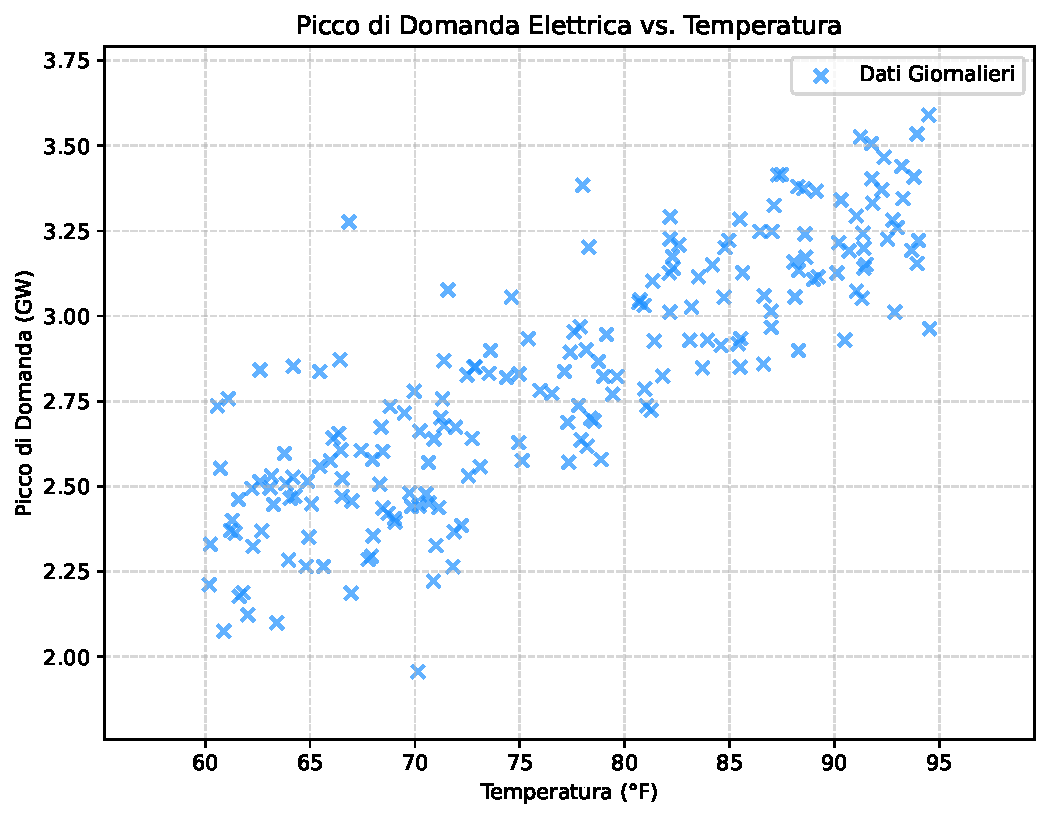
\includegraphics[width=0.7\textwidth]{images/electricity_consumption_scatter.pdf}
    \caption{Grafico a dispersione del picco di domanda di elettricità (GW) in funzione della temperatura (°F).}
    \label{fig:electricity_scatter}
\end{figure}


\subsubsection{Regressione Lineare Univariata}
Nella regressione lineare univariata, si cerca di stimare una variabile dipendente $y$ sulla base di un'unica variabile indipendente $x$. Si assume che $y$ vari in modo direttamente proporzionale ad $x$. Il valore stimato di $y$, denotato come $\hat{y}$, è quindi calcolato come:
$$ \hat{y} = \alpha \cdot x + \beta $$
Dove:
\begin{itemize}
    \item $\hat{y}$ indica una stima del valore effettivo $y$.
    \item $\alpha$ è il \textbf{coefficiente angolare} (o pendenza), che indica quanto $\hat{y}$ varia al variare di $x$.
    \item $\beta$ è l'\textbf{intercetta}, che determina il valore "base" di $\hat{y}$ quando $x$ è nullo.
\end{itemize}
L'obiettivo dell'analisi di regressione è trovare i valori dei parametri $\alpha$ e $\beta$ che rendano la stima $\hat{y}$ più accurata possibile rispetto ai valori reali $y$.

Applicato al caso studio del consumo di elettricità, assumiamo che il consumo si possa stimare come:
$$ \text{consumo}_{\text{stimato}} = \alpha \cdot \text{temperatura} + \beta $$
Qui, $\alpha$ rappresenta il tasso con cui il consumo cresce all'aumentare della temperatura, e $\beta$ rappresenta la quota "base" di consumo non dipendente dalla temperatura (es. dall'aria condizionata).  Questa funzione può essere rappresentata nel grafico a dispersione come una retta che approssima i dati osservati.

\begin{figure}[H]
    \centering
    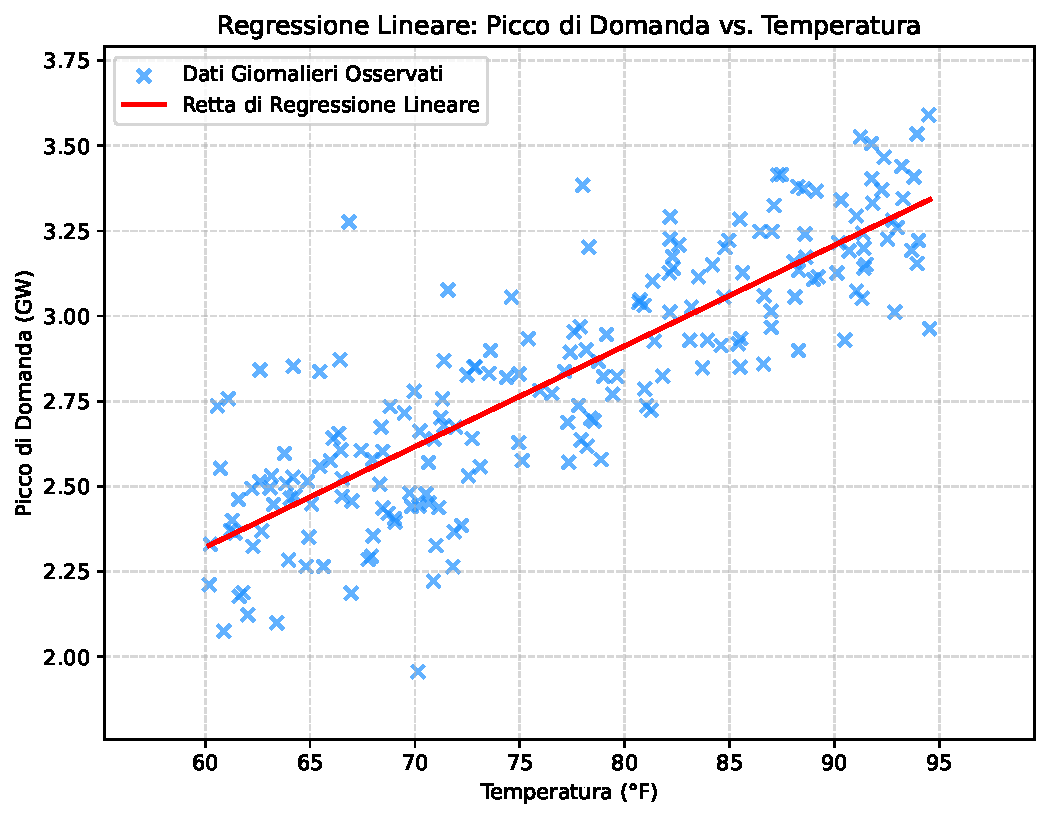
\includegraphics[width=0.7\textwidth]{images/electricity_scatter_with_line.pdf}
    \caption{Retta di regressione che approssima la relazione tra temperatura e consumo di elettricità.}
    \label{fig:electricity_scatter_line}
\end{figure}

\subsubsection{Determinare i Parametri del Modello e Misura dell'Errore}
Se disponiamo di una previsione affidabile della temperatura $t$ del giorno successivo, possiamo stimare il picco di consumo con $\alpha \cdot t + \beta$. Ma come determinare i valori ottimali per $\alpha$ e $\beta$?
Non esiste, in genere, una combinazione di valori "perfetta" che modelli esattamente tutti i dati storici.  Dobbiamo quindi individuare i valori che forniscano la migliore approssimazione possibile.

Per fare ciò, definiamo l'\textbf{errore} (o \textbf{residuo}) per ogni singola osservazione $i$ come la differenza tra il valore reale $y_i$ e il valore predetto $\hat{y}_i$:
$$ \text{errore}_i = \hat{y}_i - y_i $$
Minori sono queste differenze, migliore è l'approssimazione del modello.

Per misurare l'errore complessivo del modello su un insieme di $m$ osservazioni, una delle misure più comuni è la \textbf{Media dei Quadrati degli Errori} (Mean Squared Error - MSE):
$$ \text{MSE} = E(\alpha, \beta) = \frac{1}{m} \sum_{i=1}^{m} (\hat{y}_i - y_i)^2 $$
Sostituendo $\hat{y}_i = \alpha \cdot x_i + \beta$, la funzione d'errore $E(\alpha, \beta)$ diventa:
$$ E(\alpha, \beta) = \frac{1}{m} \sum_{i=1}^{m} (\alpha \cdot x_i + \beta - y_i)^2 $$
L'obiettivo è trovare i valori di $\alpha$ e $\beta$ che minimizzano questa funzione d'errore $E(\alpha, \beta)$.  Fissato un set di dati, $E(\alpha, \beta)$ è una funzione continua dei parametri $\alpha$ e $\beta$.  Per la regressione lineare univariata, questa funzione d'errore forma una superficie tridimensionale con una forma paraboloide convessa, il che garantisce l'esistenza di un unico minimo globale.

\begin{figure}[H]
    \centering
    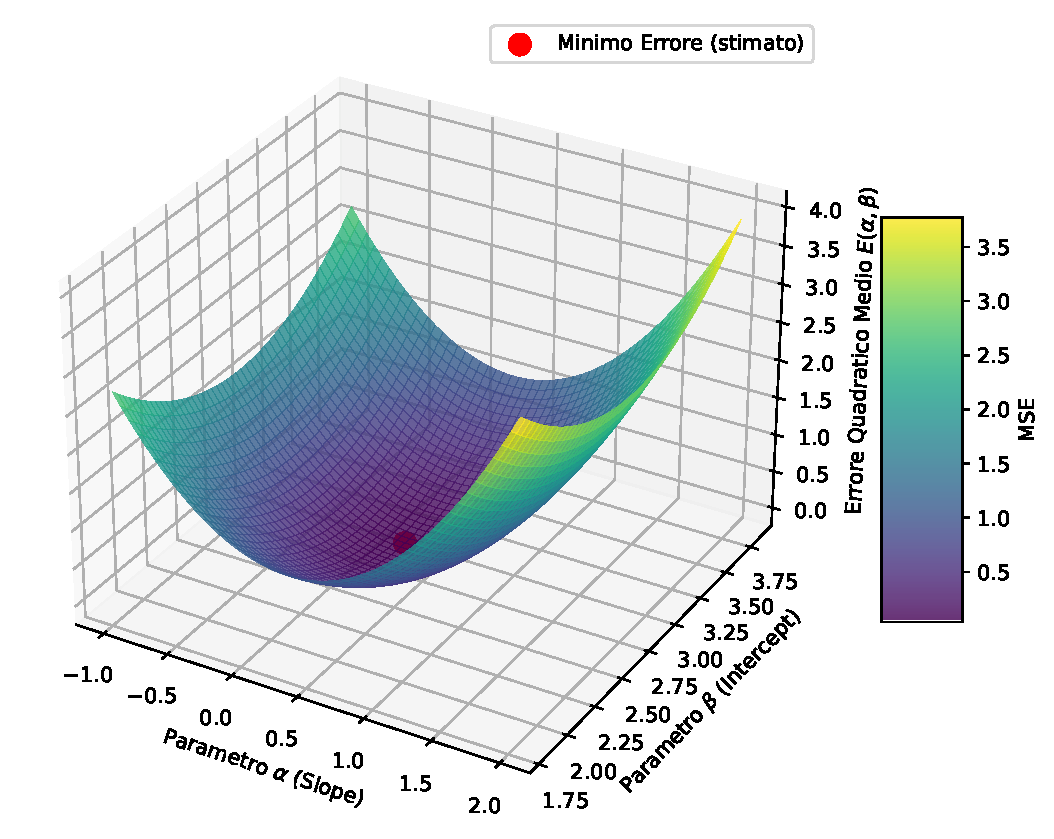
\includegraphics[width=0.6\textwidth]{images/error_function_3d.pdf}
    \caption{Visualizzazione della funzione d'errore $E(\alpha, \beta)$ come superficie tridimensionale.}
    \label{fig:error_function_3d}
\end{figure}

\subsubsection{Ottimizzazione dei Parametri: Discesa del Gradiente}
La \textbf{discesa del gradiente} (Gradient Descent) è un metodo iterativo utilizzato per trovare un minimo (locale o globale) di una funzione "seguendo" la direzione opposta al suo gradiente.

\begin{definitionbox}{Gradiente di una Funzione}
    Data una funzione $f$ a più variabili, la \textbf{derivata parziale} rispetto a una di esse è la derivata di $f$ considerando le altre variabili come costanti.
    Il \textbf{gradiente} $\nabla f$ è il vettore delle derivate parziali della funzione $f$ per ciascuna delle sue variabili.  Intuitivamente, il gradiente $\nabla f(x)$ calcolato in un punto $x$ indica la direzione e la pendenza della massima crescita della curva nel punto stesso.  Di conseguenza, la direzione $-\nabla f(x)$ (opposta al gradiente) è quella di massima decrescita.
\end{definitionbox}

L'algoritmo della discesa del gradiente procede come segue:
\begin{enumerate}
    \item Si inizia da un punto $x_0$ (cioè una combinazione iniziale dei parametri $\alpha_0, \beta_0$) scelto casualmente o con un criterio specifico.
    \item Si calcola il gradiente della funzione d'errore $\nabla E$ nel punto corrente $x_k$ (cioè con i valori $\alpha_k, \beta_k$).
    \item Si aggiornano i parametri muovendosi nella direzione opposta al gradiente per ottenere un nuovo punto $x_{k+1}$ (cioè $\alpha_{k+1}, \beta_{k+1}$) dove ci si aspetta che il valore della funzione d'errore sia minore: $E(x_{k+1}) < E(x_k)$. La formula di aggiornamento è:
          $$ x_{k+1} = x_k - \eta \cdot \nabla E(x_k) $$
          dove $\eta$ è il \textbf{tasso di apprendimento} (learning rate), un iperparametro che controlla la dimensione del "passo" ad ogni iterazione.
          \begin{itemize}
              \item Se $\eta$ è troppo basso, l'algoritmo converge lentamente.
              \item Se $\eta$ è troppo alto, l'algoritmo potrebbe "saltare" il minimo o divergere.
          \end{itemize}
    \item Si ripete dal punto 2 fino a convergenza (es. quando i parametri cambiano minimamente o si raggiunge un numero massimo di iterazioni).
\end{enumerate}

\begin{figure}[H]
    \centering
    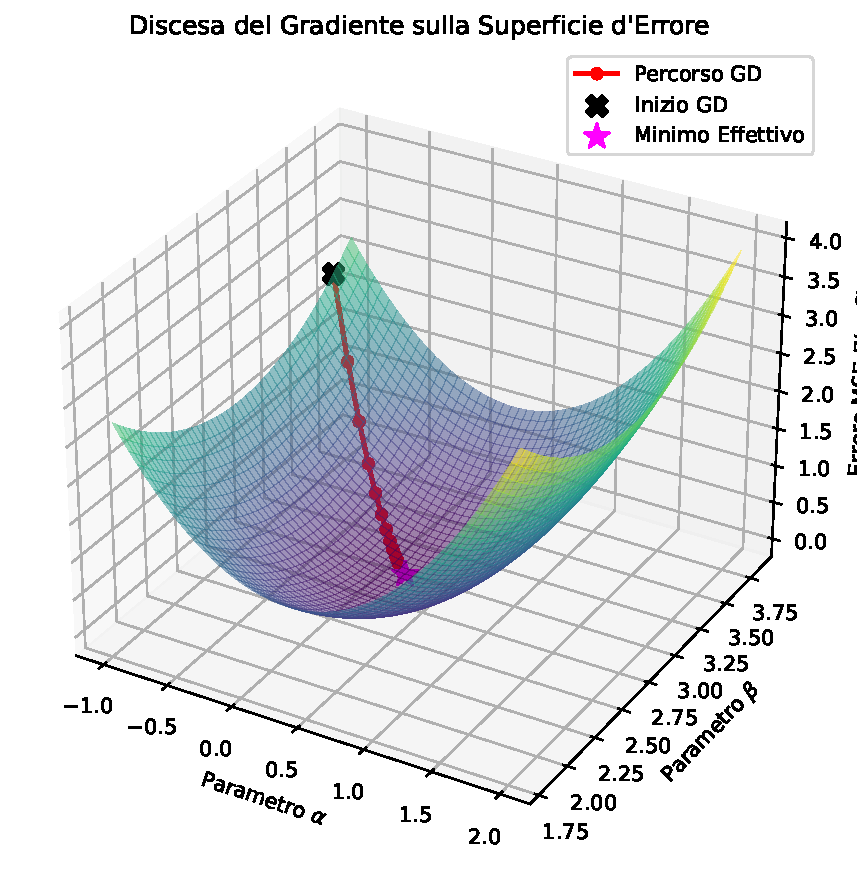
\includegraphics[width=0.6\textwidth]{images/gradient_descent_steps.pdf}
    \caption{Illustrazione della discesa del gradiente sulla curva della funzione d'errore.}
    \label{fig:gradient_descent_steps}
\end{figure}

Per la regressione lineare univariata, la funzione d'errore è $E(\alpha, \beta) = \frac{1}{m} \sum_{i=1}^{m} (\alpha x_i + \beta - y_i)^2$. Le derivate parziali rispetto ad $\alpha$ e $\beta$ sono:
$$ \frac{\partial E}{\partial \alpha} = \frac{1}{m} \sum_{i=1}^{m} 2 (\alpha x_i + \beta - y_i) \cdot x_i = \frac{2}{m} \sum_{i=1}^{m} (\hat{y}_i - y_i) x_i $$
$$ \frac{\partial E}{\partial \beta} = \frac{1}{m} \sum_{i=1}^{m} 2 (\alpha x_i + \beta - y_i) \cdot 1 = \frac{2}{m} \sum_{i=1}^{m} (\hat{y}_i - y_i) $$
Ad ogni $k$-esima iterazione della discesa del gradiente, i parametri $\alpha$ e $\beta$ vengono aggiornati come segue:
$$ \alpha_{k+1} \leftarrow \alpha_k - \eta \frac{2}{m} \sum_{i=1}^{m} (\alpha_k x_i + \beta_k - y_i) x_i $$
$$ \beta_{k+1} \leftarrow \beta_k - \eta \frac{2}{m} \sum_{i=1}^{m} (\alpha_k x_i + \beta_k - y_i) $$

Visualizzando la retta di regressione con i parametri aggiornati alle varie iterazioni, si osserva come essa approssimi progressivamente sempre meglio i dati.


\begin{figure}[H]
    \centering
    \begin{subfigure}[b]{0.45\textwidth}
        \centering
        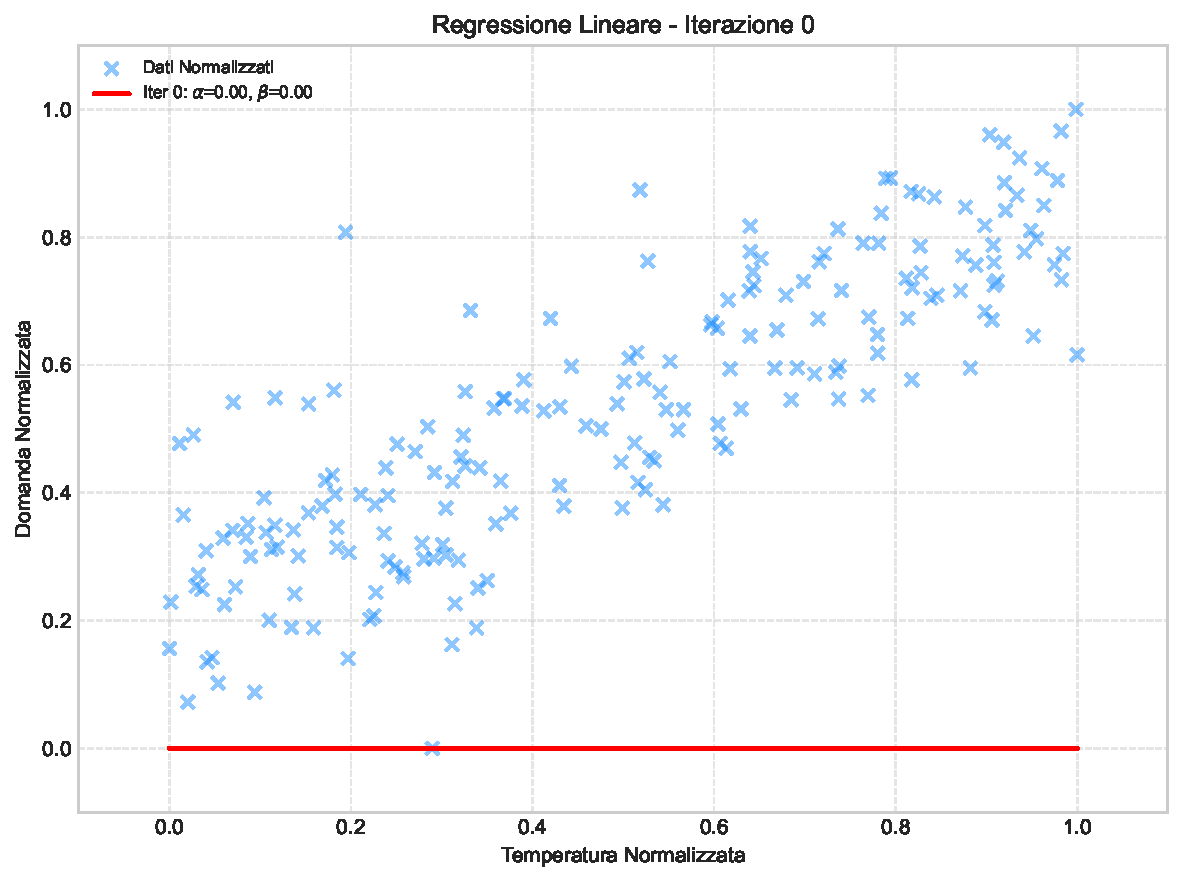
\includegraphics[width=\textwidth]{images/regression_iteration_0.pdf}
        \caption{Parametri iniziali ($\alpha=0, \beta=0$).}
    \end{subfigure}
    \hfill
    \begin{subfigure}[b]{0.45\textwidth}
        \centering
        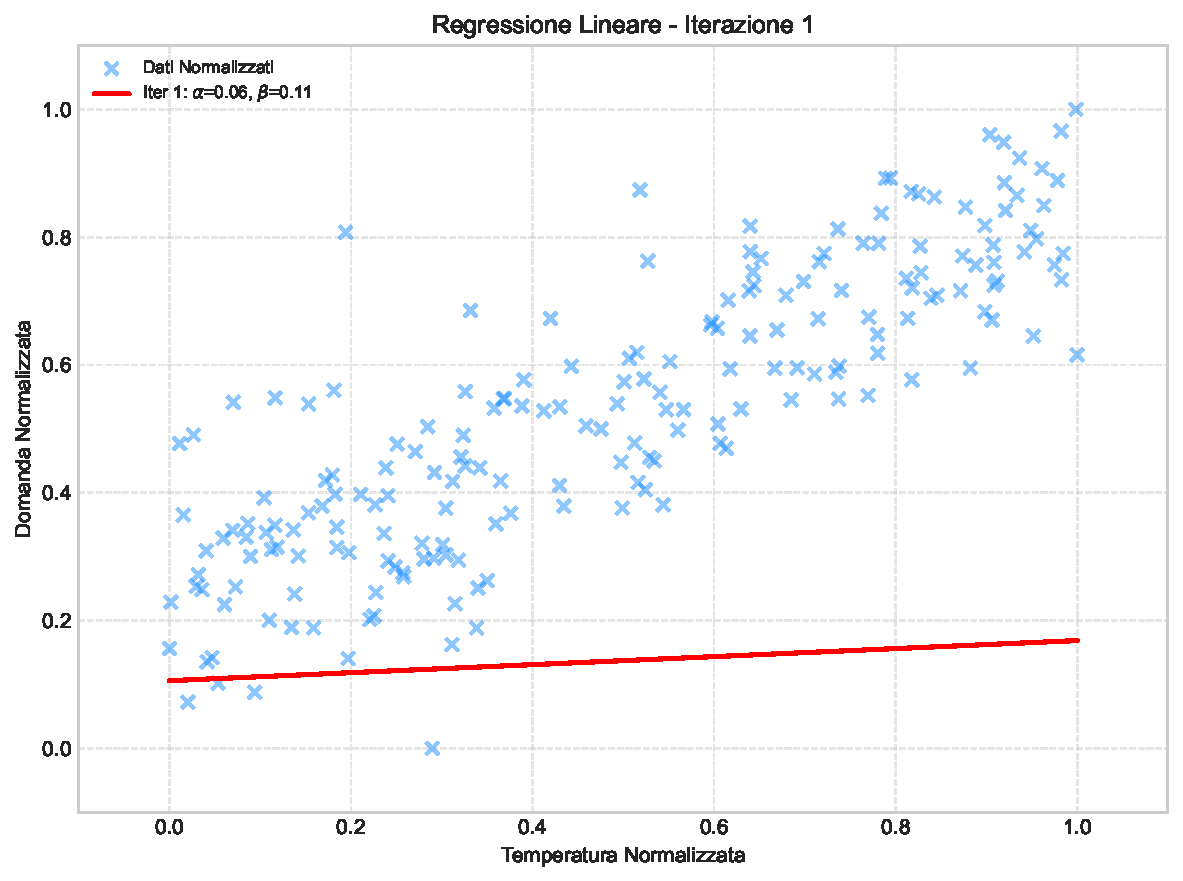
\includegraphics[width=\textwidth]{images/regression_iteration_1.pdf}
        \caption{Dopo 1 iterazione.}
    \end{subfigure}
    \vskip\baselineskip
    \begin{subfigure}[b]{0.45\textwidth}
        \centering
        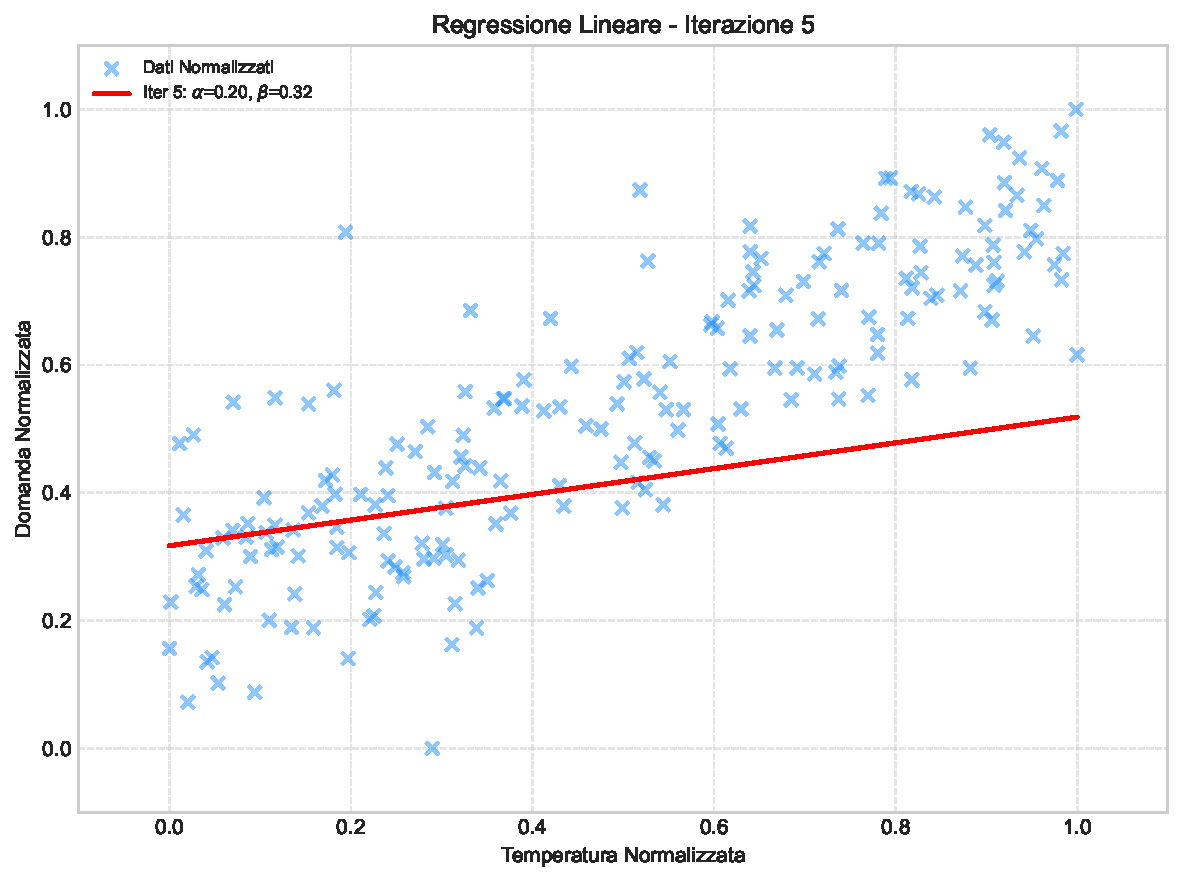
\includegraphics[width=\textwidth]{images/regression_iteration_5.pdf}
        \caption{Dopo 5 iterazioni.}
    \end{subfigure}
    \hfill
    \begin{subfigure}[b]{0.45\textwidth}
        \centering
        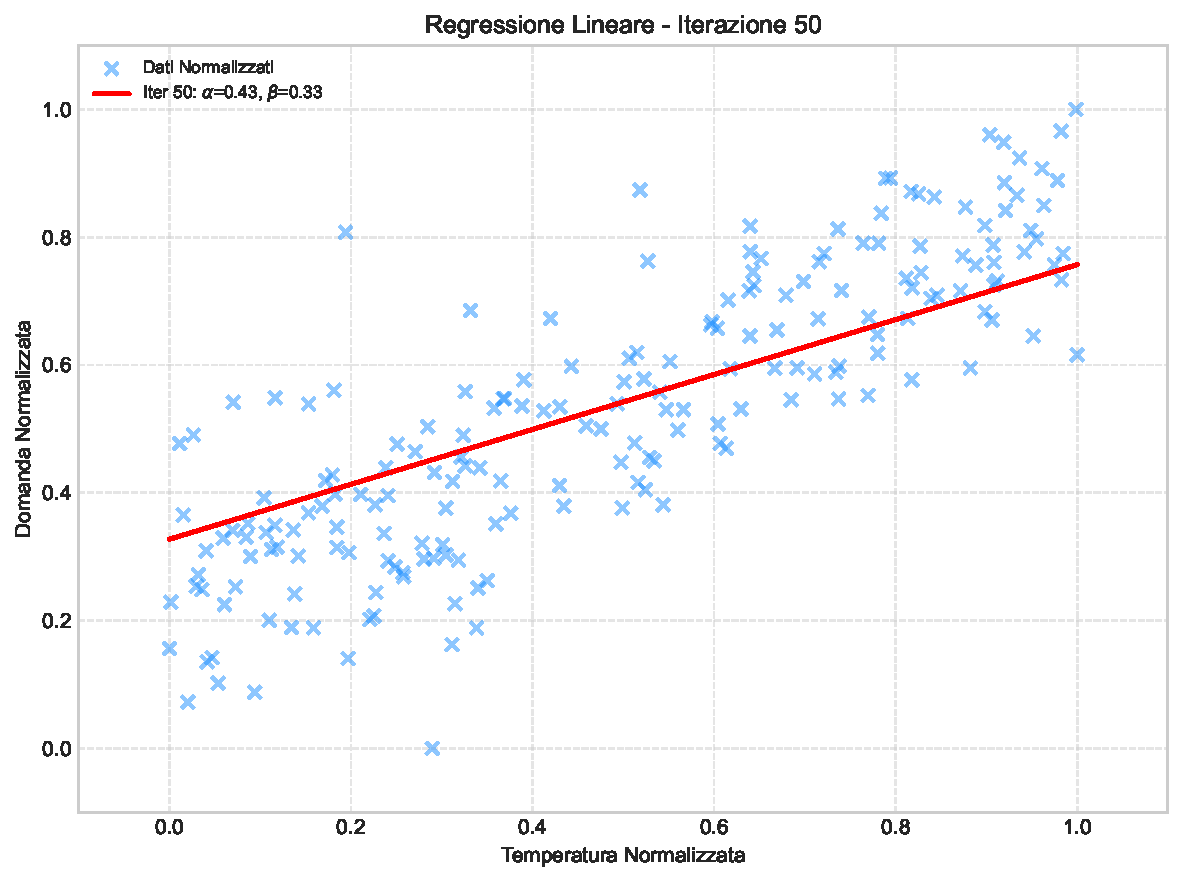
\includegraphics[width=\textwidth]{images/regression_iteration_50.pdf}
        \caption{Dopo 50 iterazioni.}
    \end{subfigure}
    \caption{Progressione del modello di regressione durante la discesa del gradiente (dati normalizzati).}
    \label{fig:regression_progression}
\end{figure}


\subsection{Regressione Lineare Multivariata}
Con la regressione lineare multivariata si stima una variabile dipendente $y$ sulla base di più variabili indipendenti $x_1, \dots, x_n$. La previsione può avvenire a partire da un numero arbitrario di variabili numeriche e categoriche.

\begin{notebox}{Gestione delle Variabili Categoriche}
    Ogni variabile categorica deve essere convertita in più variabili binarie (0 o 1). Si crea una nuova variabile binaria per ciascun valore possibile della variabile categorica originale (tecnica nota come \textit{one-hot encoding}). Ad esempio, se una variabile "quartiere" ha valori $\{q1, q2, q3\}$, questa viene trasformata in tre nuove variabili: $x_{q1}$ (1 se quartiere è q1, 0 altrimenti), $x_{q2}$ (1 se quartiere è q2, 0 altrimenti), e $x_{q3}$ (1 se quartiere è q3, 0 altrimenti).
\end{notebox}

Nel caso della regressione lineare multivariata, la forma della funzione stimata $\hat{y} = h_{\theta}(x_1, \dots, x_n)$ è un iperpiano in uno spazio a $n+1$ dimensioni:
$$ \hat{y} = h_{\theta}(x_1, \dots, x_n) = \theta_0 + \theta_1 x_1 + \theta_2 x_2 + \dots + \theta_n x_n $$
Dove:
\begin{itemize}
    \item $\theta_0$ è l'intercetta.
    \item $\theta_1, \dots, \theta_n$ sono i coefficienti angolari (o pesi), ciascuno dei quali indica il "peso" della rispettiva variabile $x_j$ nella previsione.
\end{itemize}

\paragraph{Stima dei Prezzi delle Case} Un'agenzia immobiliare desidera stimare i prezzi ideali per le case in vendita, basandosi su dati storici di case vendute in precedenza, che includono caratteristiche come numero di stanze, metratura, quartiere, e il prezzo di vendita finale. L'obiettivo è creare un'applicazione che stimi automaticamente il prezzo per massimizzare i profitti e ridurre i tempi di vendita.
Ad esempio, per una casa con determinate caratteristiche (es. 3 camere, 2000 mq, quartiere Hipsterton), si vuole predire il prezzo. Mentre un addetto esperto usa regole empiriche, la regressione può automatizzare e potenzialmente migliorare questo processo.

Con la regressione lineare, il prezzo della casa $P$ viene considerato come una somma pesata delle sue caratteristiche $s$ (metratura), $n_b$ (numero di stanze da letto), e $q$ (quartiere, opportunamente binarizzato):
$$ P(n_b, s, q) = \theta_0 + \theta_1 n_b + \theta_2 s + \sum_{k} (\theta_k \cdot \text{is\_quartiere}_k(q)) $$
dove i parametri $\theta$ sono da apprendere.

\subsubsection{Notazione Vettoriale}
Il modello generale di regressione lineare multivariata $h_{\theta}(x_1, \dots, x_n) = \theta_0 + \theta_1 x_1 + \dots + \theta_n x_n$ può essere scritto in forma vettoriale più compatta. Definiamo un vettore delle variabili indipendenti $x = [x_1, x_2, \dots, x_n]^T$ e un vettore dei parametri $\theta = [\theta_1, \theta_2, \dots, \theta_n]^T$. Il modello può essere scritto come $h_{\theta}(x) = \theta_0 + \theta^T x$.

Per includere anche l'intercetta $\theta_0$ nel prodotto vettoriale, si aggiunge una componente $x_0 = 1$ al vettore delle features $x$, ottenendo $x = [x_0, x_1, \dots, x_n]^T = [1, x_1, \dots, x_n]^T$. Il vettore dei parametri diventa $\theta = [\theta_0, \theta_1, \dots, \theta_n]^T$.
Il modello si riduce così a un prodotto scalare tra vettori:
$$ h_{\theta}(x) = \theta^T x = \theta_0 x_0 + \theta_1 x_1 + \dots + \theta_n x_n = [\theta_0 \quad \theta_1 \quad \dots \quad \theta_n] \begin{bmatrix} 1 \\ x_1 \\ \vdots \\ x_n \end{bmatrix} $$

\subsubsection{Funzione d'Errore per Regressione Multivariata}
Analogamente al caso univariato, la funzione d'errore (MSE) per la regressione multivariata, dato un set di $m$ osservazioni, è:
$$ E(\theta_0, \theta_1, \dots, \theta_n) = \frac{1}{m} \sum_{i=1}^{m} (h_{\theta}(x^{(i)}) - y^{(i)})^2 = \frac{1}{m} \sum_{i=1}^{m} \left( \theta_0 + \sum_{j=1}^{n} \theta_j x_j^{(i)} - y^{(i)} \right)^2 $$
dove $x^{(i)}$ è il vettore delle features per la $i$-esima osservazione e $y^{(i)}$ è il valore reale corrispondente.
In forma vettoriale compatta, utilizzando $x^{(i)}$ che include $x_0=1$:
$$ E(\theta) = \frac{1}{m} \sum_{i=1}^{m} (\theta^T x^{(i)} - y^{(i)})^2 $$

\subsubsection{Discesa del Gradiente per Regressione Multivariata}
Per minimizzare $E(\theta)$, si calcola la derivata parziale della funzione d'errore rispetto a ciascun parametro $\theta_p$ (per $p=0, \dots, n$):
$$ \frac{\partial E(\theta)}{\partial \theta_p} = \frac{2}{m} \sum_{i=1}^{m} (h_{\theta}(x^{(i)}) - y^{(i)}) \cdot x_p^{(i)} $$
(ricordando che $x_0^{(i)} = 1$ per la derivata rispetto a $\theta_0$).

L'aggiornamento iterativo per ciascun parametro $\theta_p$ nella discesa del gradiente è:
$$ \theta_{p, k+1} \leftarrow \theta_{p, k} - \eta \frac{2}{m} \sum_{i=1}^{m} (h_{\theta_k}(x^{(i)}) - y^{(i)}) \cdot x_p^{(i)} $$

\subsubsection{Notazione Matriciale per il Dataset e la Discesa del Gradiente}
L'intero insieme di $m$ osservazioni può essere rappresentato da una matrice $X$ ($m \times (n+1)$) degli input e un vettore colonna $y$ ($m \times 1$) degli output attesi.
La matrice $X$ ha una riga per ogni osservazione e una colonna per ogni feature, più una colonna di uni per l'intercetta $\theta_0$.
$$ X = \begin{pmatrix}
        (x^{(1)})^T \\
        (x^{(2)})^T \\
        \vdots      \\
        (x^{(m)})^T
    \end{pmatrix} = \begin{pmatrix}
        1      & x_1^{(1)} & x_2^{(1)} & \dots  & x_n^{(1)} \\
        1      & x_1^{(2)} & x_2^{(2)} & \dots  & x_n^{(2)} \\
        \vdots & \vdots    & \vdots    & \ddots & \vdots    \\
        1      & x_1^{(m)} & x_2^{(m)} & \dots  & x_n^{(m)}
    \end{pmatrix}, \quad y = \begin{pmatrix}
        y^{(1)} \\
        y^{(2)} \\
        \vdots  \\
        y^{(m)}
    \end{pmatrix}, \quad \theta = \begin{pmatrix}
        \theta_0 \\
        \theta_1 \\
        \vdots   \\
        \theta_n
    \end{pmatrix} $$

Con questa notazione, il vettore delle predizioni è $X\theta$. Il vettore dei residui è $X\theta - y$.
Il gradiente della funzione d'errore $E(\theta)$ può essere espresso in forma vettoriale/matriciale come:
$$ \nabla E(\theta) = \frac{2}{m} X^T (X\theta - y) $$
L'aggiornamento dell'intero vettore dei parametri $\theta$ ad ogni iterazione $k$ della discesa del gradiente diventa:
$$ \theta_{k+1} \leftarrow \theta_k - \eta \frac{2}{m} X^T (X\theta_k - y) $$

\subsection{Normalizzazione dei Dati}
Le variabili coinvolte in un modello di regressione possono avere scale di valori molto diverse (es. temperature in decine di gradi, consumi energetici in unità). Questo può rendere difficile la convergenza della discesa del gradiente, poiché i parametri associati a features con range più ampi potrebbero richiedere tassi di apprendimento diversi o dominare gli aggiornamenti.
Una soluzione comune è la \textbf{normalizzazione dei dati}, che trasforma tutte le variabili in un intervallo comune, ad esempio $[0, 1]$.
Una tecnica comune è la normalizzazione min-max: dato un valore $x_j$ di una generica variabile $X_j$, il suo valore normalizzato $\tilde{x}_j$ è:
$$ \tilde{x}_j = \frac{x_j - \min(X_j)}{\max(X_j) - \min(X_j)} $$
È comune normalizzare tutte le variabili, inclusa la variabile dipendente, prima di addestrare il modello.
Addestrando un modello $h_{\tilde{\theta}}(\tilde{x}) = \tilde{\theta}^T \tilde{x}$ su dati normalizzati, i parametri $\tilde{\theta}$ saranno ottimizzati su questi dati. Per usare il modello, si normalizzano gli input e si denormalizzano gli output, oppure si trasformano i parametri $\tilde{\theta}$ per ottenere quelli validi sui dati originali $\theta$.

\subsection{Valutazione del Modello di Regressione}
L'obiettivo della regressione è ottenere un modello generale, capace di fare previsioni accurate su nuovi dati (non visti durante l'addestramento) con un'accuratezza simile a quella mostrata sui dati di training.
Se l'accuratezza su nuovi dati è significativamente più bassa, possono esserci due problemi principali:
\begin{itemize}
    \item Il modello è affetto da \textbf{overfitting}: è troppo aderente ai dati di addestramento e ha perso generalità. Soluzioni possono includere ridurre il numero di variabili o regolarizzare il modello.
    \item Il \textbf{training set} impiegato non è statisticamente rappresentativo delle peculiarità dei nuovi dati.
\end{itemize}
Per verificare la capacità di generalizzazione del modello, è cruciale validarlo su dati non usati per l'addestramento.

\subsubsection{Validazione con Metodo Hold-Out}
Il metodo hold-out prevede di dividere i dati a disposizione in due insiemi disgiunti:
\begin{itemize}
    \item \textbf{Training set}: Utilizzato per addestrare il modello di regressione (minimizzando l'errore su di esso).
    \item \textbf{Validation set} (o Test set): Usato dopo l'addestramento per verificare l'errore del modello su dati "ignoti" e quindi la sua capacità di generalizzazione.
\end{itemize}
Se l'errore sul validation set è simile a quello sul training set, si assume che il modello abbia generalizzato bene. Un errore sul validation set significativamente maggiore indica overfitting o che il training set non era rappresentativo.

\subsubsection{Misure di Errore Comuni}
Oltre all'Errore Quadratico Medio (MSE), funzionale all'addestramento, si usano altre metriche per valutare il modello:

\begin{definitionbox}{Mean Absolute Percentage Error (MAPE)}
    L'errore relativo tra un valore reale $y_i$ e la stima $\hat{y}_i$ è $|\frac{\hat{y}_i - y_i}{y_i}|$. Il MAPE è la media di questi errori relativi:
    $$ \text{MAPE} = \frac{1}{m} \sum_{i=1}^{m} \left| \frac{\hat{y}_i - y_i}{y_i} \right| $$
    Fornisce una misura percentuale dell'errore, che può essere più interpretabile.
\end{definitionbox}

\begin{definitionbox}{Coefficiente di Determinazione ($R^2$)}
    Il coefficiente $R^2$ indica la proporzione della varianza della variabile dipendente che è predicibile dalle variabili indipendenti. Il suo valore è compreso tra 0 e 1.
    $$ R^2 = 1 - \frac{\sum_{i=1}^{m} (y_i - \hat{y}_i)^2}{\sum_{i=1}^{m} (y_i - \bar{y})^2} = 1 - \frac{\text{MSE}}{\text{Varianza di } y} $$
    (La formula sulla slide $R^{2}=\frac{\sum_{i=1}^{m}(\hat{y}_{i}-\overline{y})^{2}}{\sum_{i=1}^{m}(y_{i}-\overline{y})^{2}}$  rappresenta la frazione di varianza spiegata dal modello).
    \begin{itemize}
        \item $R^2 = 1$ indica che il modello descrive perfettamente i dati.
        \item $R^2 = 0$ indica che non c'è alcuna relazione lineare tra il modello e i dati.
        \item Valori intermedi indicano diversi gradi di efficacia del modello.
    \end{itemize}
    $R^2$ tende ad aumentare (o rimanere uguale) all'aumentare del numero di variabili indipendenti, indipendentemente dalla loro effettiva utilità.
\end{definitionbox}

\begin{definitionbox}{$R^2$ Aggiustato ($\overline{R}^2$)}
    Per ovviare al problema dell'$R^2$ che cresce con il numero di predittori, si usa l'$R^2$ aggiustato:
    $$ \overline{R}^2 = 1 - (1 - R^2) \frac{m-1}{m-n-1} $$
    dove $m$ è il numero di osservazioni e $n$ è il numero di variabili indipendenti (predittori). $\overline{R}^2$ può essere negativo ed è sempre minore o uguale a $R^2$. Penalizza l'aggiunta di variabili inutili.
\end{definitionbox}

\begin{examplebox}{Valutazione Modello Prezzi Case}
    Dividendo i dati sulle case (70\% training, 30\% validation) e addestrando un modello di regressione lineare, si potrebbero ottenere le seguenti metriche:
    \begin{itemize}
        \item MSE (Training): $\approx 22.5$
        \item MSE (Validation): $\approx 21.5$
        \item MAPE (Training): $\approx 16.57\%$
        \item MAPE (Validation): $\approx 16.52\%$
        \item $R^2$ (Training): $\approx 0.7435$
        \item $R^2$ (Validation): $\approx 0.7112$
    \end{itemize}
    La vicinanza delle performance tra training e validation set suggerisce che il modello generalizza abbastanza bene in questo esempio.
\end{examplebox}


\subsubsection{Intervallo di Confidenza per il Coefficiente di Determinazione ($R^2$)}
È possibile calcolare un intervallo di confidenza (CI) per il coefficiente $R^2$ per stimare l'intervallo in cui è probabile che si trovi il vero valore di $R^2$ della popolazione. La formula generale per l'intervallo di confidenza è:
$$ CI = R^2 \pm t \times \sqrt{VR} $$
Dove:
\begin{itemize}
    \item $R^2$ è il coefficiente di determinazione calcolato sul campione.
    \item $t$ è il valore critico della distribuzione t di Student, che dipende dal livello di confidenza desiderato (es. 95\%) e dal numero di gradi di libertà (legato al numero di istanze $m$ del test set). Per un numero elevato di istanze (es. $m \ge 500$) e una confidenza del 95\%, $t \approx 1.965$. Il valore esatto di $t$ per un test a due code con significatività $\alpha$ e $df$ gradi di libertà si ottiene con funzioni statistiche (es. stats.t.ppf(1 - alpha/2, df)).
    \item $\sqrt{VR}$ è l'errore standard di $R^2$. La varianza $VR$ di $R^2$ può essere calcolata con la formula:
          $$ VR = \frac{4 R^2 (1-R^2)^2 (m-n-1)^2}{(m^2-1)(m+3)} $$
          dove $m$ è il numero di istanze del test set e $n$ è il numero di variabili indipendenti (predittori).
\end{itemize}
Questo intervallo fornisce una misura dell'incertezza associata alla stima puntuale di $R^2$.

\subsection{Classificazione di Opinioni Positive e Negative}
La regressione lineare può essere adattata anche per problemi che, a prima vista, sembrano di classificazione, come la sentiment analysis, ovvero l'identificazione della polarità (positiva, negativa, o neutra) di un testo.

Le persone pubblicano comunemente online opinioni riguardo a prodotti, servizi, hotel, ecc.. A volte, come nelle recensioni Amazon, l'utente associa un voto (es. da 1 a 5 stelle). L'obiettivo è stimare automaticamente questo voto (o una polarità derivata) partendo solo dal testo dell'opinione, ad esempio per analizzare rapidamente migliaia di recensioni.

\subsubsection{Feature Engineering da Testo}
Per applicare la regressione a dati testuali, è necessario prima trasformare il testo in feature numeriche. Un approccio semplice si basa sull'utilizzo di dizionari di parole:
\begin{itemize}
    \item Si predispongono liste di parole con connotazione intrinsecamente positiva (es. "great", "wonderful", "awesome") e negativa (es. "horrible", "useless", "sad").
    \item Dato il testo di una recensione, si contano quante parole di ciascuna lista sono presenti.
    \item Questi conteggi (es. "$pos\_words$", "$neg\_words$") diventano le variabili numeriche (features) che caratterizzano ciascuna recensione.
\end{itemize}
Ad esempio, la recensione "Wonderful! A really great movie despite a sad ending" potrebbe avere $pos\_words$ = 2 (wonderful, great) e $neg\_words$ = 1 (sad).

\subsubsection{Definizione del Modello di Regressione per la Stima del Voto}
Disponendo di un dataset di recensioni con il testo e il voto associato (es. numero di stelle), possiamo prima calcolare le features $pos\_words$ e $neg\_words$ per ogni recensione.
Successivamente, si può addestrare un modello di regressione lineare multivariata per stimare il voto (es. stars) utilizzando queste due variabili:
$$ \text{stars}_{\text{stimate}} = \theta_0 + \theta_1 \cdot \text{pos\_words} + \theta_2 \cdot \text{neg\_words} $$
I parametri $\theta_0, \theta_1, \theta_2$ vengono appresi dall'algoritmo di regressione (es. minimizzando l'MSE sui dati di training).

\subsubsection{Interpretabilità del Modello (Explainability)}
Una volta addestrato il modello, i valori dei coefficienti $\theta$ offrono interpretabilità (explainability):
\begin{itemize}
    \item $\theta_0$ (intercetta): Rappresenta il voto base stimato quando i conteggi delle parole positive e negative sono zero.
    \item $\theta_1$: Indica di quanto aumenta (se positivo) o diminuisce (se negativo) il voto stimato per ogni parola positiva aggiuntiva, a parità di parole negative.
    \item $\theta_2$: Indica di quanto aumenta (se positivo) o diminuisce (se negativo) il voto stimato per ogni parola negativa aggiuntiva, a parità di parole positive.
\end{itemize}
Ad esempio, se i coefficienti appresi fossero $\theta_0 \approx 3.99$, $\theta_1 \approx 0.034$, $\theta_2 \approx -0.042$, significherebbe che si parte da un voto base di circa 4 stelle; ogni parola positiva aggiunge circa 0.035 stelle, mentre ogni parola negativa sottrae circa 0.042 stelle.
Questa capacità di interpretare i modelli è molto importante, specialmente in domini critici, a differenza di alcuni metodi più complessi come le reti neurali profonde ("black box").

\subsubsection{Utilizzo della Regressione per la Classificazione e Valutazione}
Anche se la regressione produce un output continuo (il voto stimato), può essere usata per compiti di classificazione binaria (o multi-classe) applicando una soglia.
Ad esempio, si possono classificare le recensioni come "positive" se il voto stimato è $\ge 3.5$ stelle, e "negative" altrimenti.
L'accuratezza del classificatore può essere quindi calcolata confrontando le etichette predette con quelle reali (derivate dai voti reali) sul validation set:
$$ \text{Accuratezza} = \frac{\text{Numero di classificazioni corrette}}{\text{Numero totale di recensioni}} $$
Ad esempio, si potrebbe ottenere un'accuratezza del 73.65\%. L'accuratezza potrebbe variare escludendo casi ambigui (es. recensioni neutre).



\section{Regressione Non Lineare}

Mentre la regressione lineare modella una relazione lineare tra le variabili indipendenti e la variabile dipendente, molti fenomeni del mondo reale presentano andamenti più complessi. La regressione non lineare generalizza questo approccio per catturare tali relazioni.

\subsection{Regressione Polinomiale}
La regressione polinomiale è una forma di regressione lineare in cui la relazione tra la variabile indipendente $x$ e la variabile dipendente $y$ è modellata come un polinomio di grado $g$ in $x$. Questo permette di adattare modelli più flessibili a dati che non seguono un andamento strettamente lineare.

Per una singola variabile indipendente $x$, un modello polinomiale di grado $g$ è dato da:
$$ \hat{y} = h_{\theta}(x) = \theta_0 + \theta_1 x + \theta_2 x^2 + \dots + \theta_g x^g $$
Ad esempio, un modello polinomiale di grado 3 ha 4 termini (e quindi 4 parametri $\theta_i$):
$$ \hat{y} = \theta_0 + \theta_1 x + \theta_2 x^2 + \theta_3 x^3 $$
Se si considerano due variabili indipendenti, $a$ e $b$, un modello polinomiale di grado 2 include termini per $a$, $b$, $a^2$, $b^2$ e il termine di interazione $ab$:
$$ h(a,b) = \theta_0 + \theta_1 a + \theta_2 a^2 + \theta_3 b + \theta_4 ab + \theta_5 b^2 $$

\begin{notebox}{Linearità rispetto ai Parametri}
    È importante notare che la regressione polinomiale è ancora considerata un tipo di regressione \textbf{lineare} dal punto di vista dei parametri $\theta_j$. Sebbene la relazione con le variabili originali $x$ (o $a, b$) sia non lineare, il modello è lineare nei coefficienti $\theta_j$ che devono essere stimati. Questo significa che le tecniche usate per la regressione lineare (come la minimizzazione dell'MSE e la discesa del gradiente) possono essere applicate anche qui, considerando le potenze di $x$ (es. $x, x^2, x^3$) come nuove feature. La funzione d'errore è definita in uno spazio a maggiori dimensioni (corrispondenti al numero di parametri $\theta_j$), ma l'algoritmo di regressione rimane concettualmente lo stesso della regressione lineare semplice.
\end{notebox}

\subsubsection{Esempio: Predizione del Consumo di Elettricità sull'Intero Anno}
Precedentemente si è analizzata la predizione dei consumi elettrici nei mesi estivi. Tuttavia, ci si aspetta un aumento dei consumi anche nei mesi più freddi a causa del riscaldamento elettrico. Visualizzando i dati di consumo sull'intero anno in funzione della temperatura, si osserva spesso un andamento non lineare (ad esempio, a forma di "U" o parabola), con consumi elevati sia a basse che ad alte temperature.

\begin{figure}[H]
    \centering
    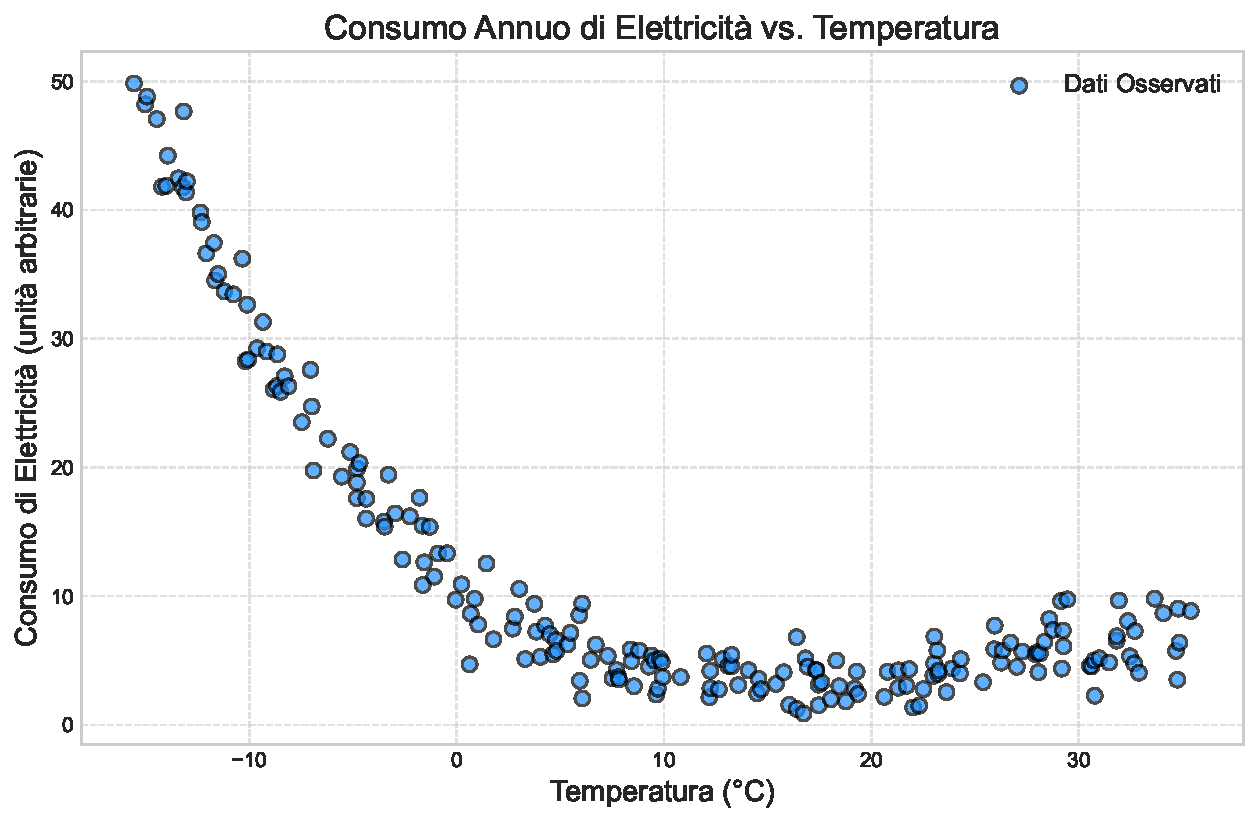
\includegraphics[width=0.7\textwidth]{images/electricity_yearly_scatter.pdf}
    \caption{Consumo di elettricità (demand) in funzione della temperatura (temp) sull'intero anno, mostrando un andamento non lineare.}
    \label{fig:electricity_yearly_scatter}
\end{figure}

Se si addestra un modello di regressione lineare semplice su questi dati, l'approssimazione può risultare inaccurata, portando a un errore quadratico medio elevato e un basso coefficiente $R^2$. Ad esempio, si potrebbe ottenere un $R^2$ di $0.028$, indicando che la retta non approssima bene i dati.

\begin{figure}[H]
    \centering
    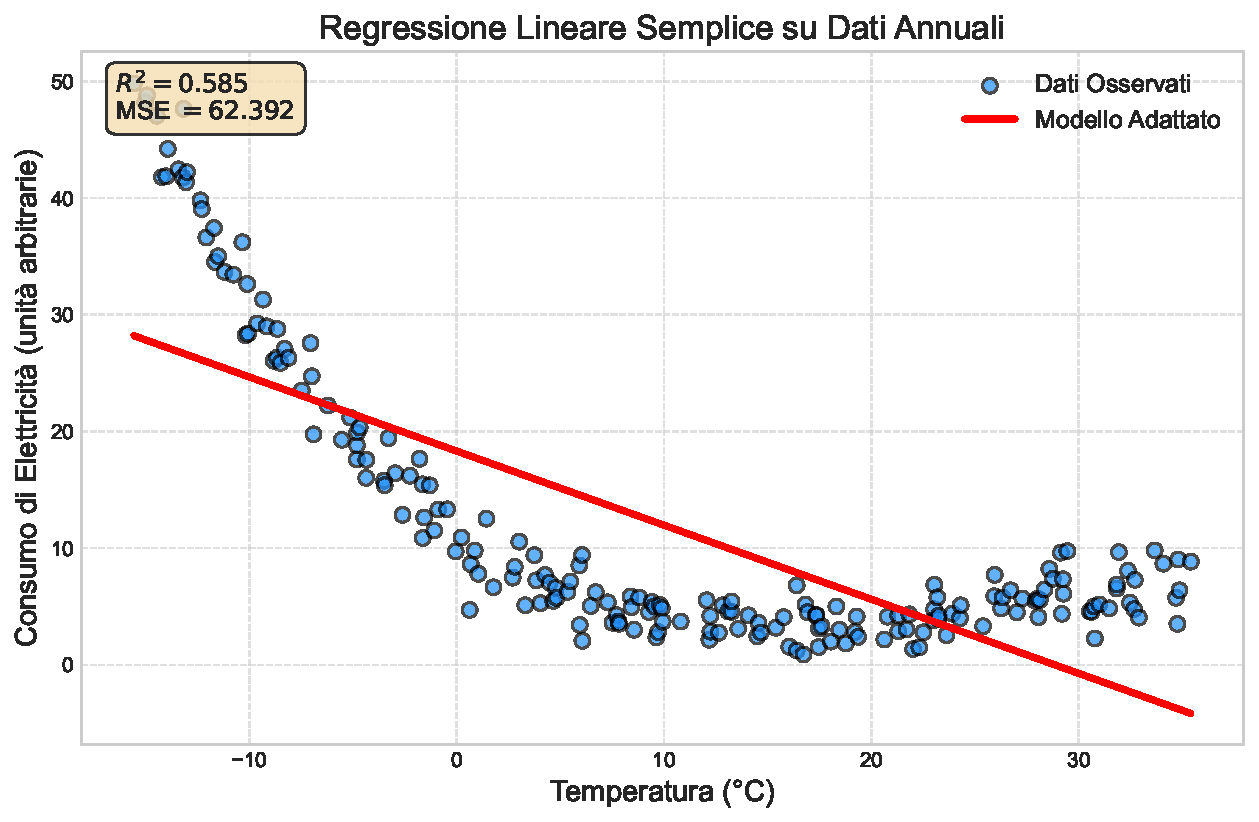
\includegraphics[width=0.7\textwidth]{images/electricity_yearly_linear_fit.pdf}
    \caption{Tentativo di approssimare i consumi annuali con una regressione lineare semplice.}
    \label{fig:electricity_yearly_linear_fit}
\end{figure}

\subsubsection{Regressione Polinomiale di $2^{\circ}$ Grado per i Consumi}
Utilizzando un modello polinomiale di secondo grado, la stima del consumo $y$ (demand) in base alla temperatura $x$ (temp) diventa:
$$ \hat{y} = \theta_0 + \theta_1 x + \theta_2 x^2 $$
La funzione d'errore quadratico medio da minimizzare è:
$$ E(\theta_0, \theta_1, \theta_2) = \frac{1}{m} \sum_{i=1}^{m} (\theta_0 + \theta_1 x_i + \theta_2 x_i^2 - y_i)^2 $$
Per trovare i parametri ottimali $\theta_0, \theta_1, \theta_2$, si calcolano le derivate parziali di $E(\theta)$ rispetto a ciascun parametro e si applica la discesa del gradiente. Le derivate parziali sono:
$$ \frac{\partial E}{\partial \theta_0} = \frac{2}{m} \sum_{i=1}^{m} (\theta_0 + \theta_1 x_i + \theta_2 x_i^2 - y_i) $$
$$ \frac{\partial E}{\partial \theta_1} = \frac{2}{m} \sum_{i=1}^{m} (\theta_0 + \theta_1 x_i + \theta_2 x_i^2 - y_i) x_i $$
$$ \frac{\partial E}{\partial \theta_2} = \frac{2}{m} \sum_{i=1}^{m} (\theta_0 + \theta_1 x_i + \theta_2 x_i^2 - y_i) x_i^2 $$
Un modello di secondo grado corrisponde graficamente a una parabola. Per i dati di consumo elettrico annuale, una parabola può approssimare i dati in modo significativamente migliore rispetto a una retta, risultando in un errore quadratico medio inferiore (es. 0.036) e un $R^2$ più alto (es. 0.566).

\begin{figure}[H]
    \centering
    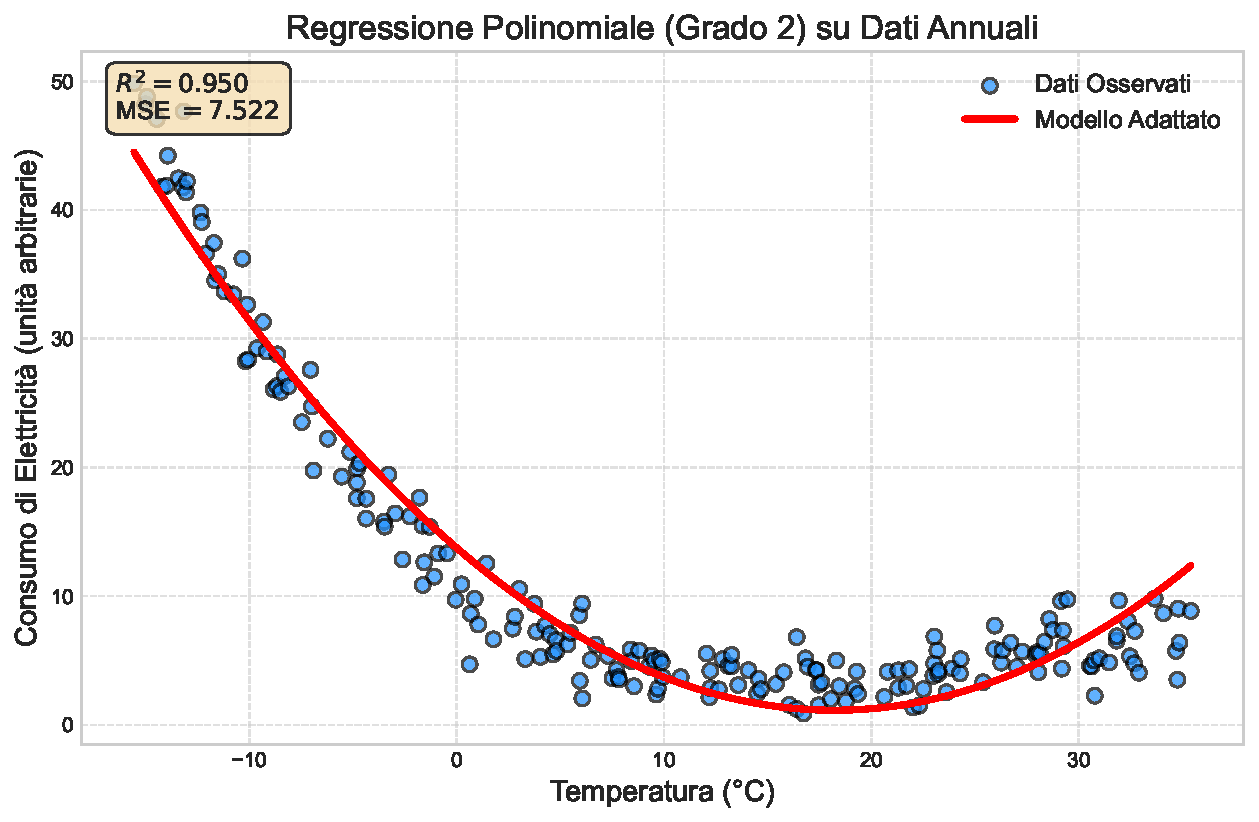
\includegraphics[width=0.7\textwidth]{images/electricity_yearly_poly2_fit.pdf}
    \caption{Approssimazione dei consumi annuali con una regressione polinomiale di $2^{\circ}$ grado.}
    \label{fig:electricity_yearly_poly2_fit}
\end{figure}

\subsubsection{Regressione Polinomiale di Grado Superiore}
Aumentando ulteriormente il grado del polinomio, ad esempio a $3^{\circ}$ grado ($\hat{y} = \theta_0 + \theta_1 x + \theta_2 x^2 + \theta_3 x^3$), la curva del modello può diventare ancora più flessibile e adattarsi meglio ai dati. Per i consumi elettrici, un modello di $3^{\circ}$ grado potrebbe migliorare ulteriormente le metriche (es. MSE a 0.025, $R^2$ a 0.703). Anche un polinomio di grado 10 potrebbe portare a miglioramenti.

\begin{figure}[H]
    \centering
    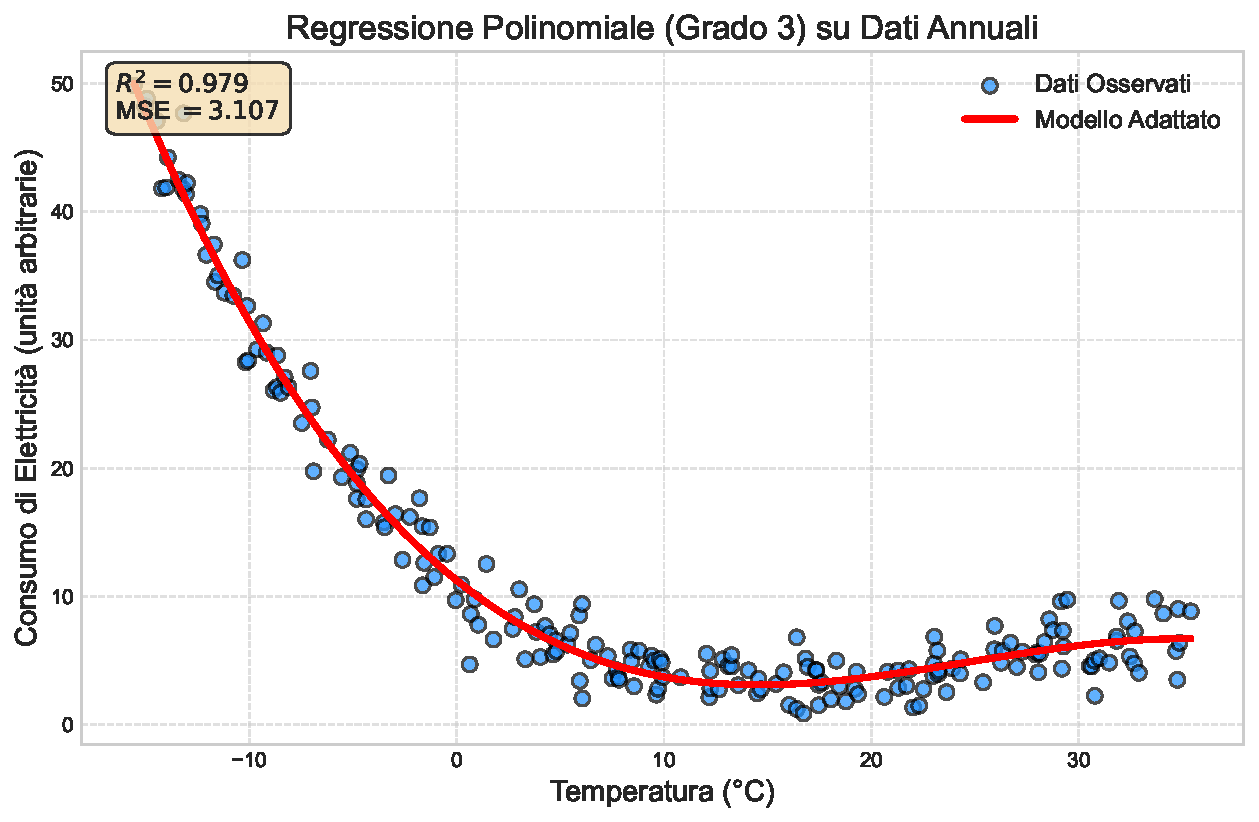
\includegraphics[width=0.7\textwidth]{images/electricity_yearly_poly3_fit.pdf}
    \caption{Approssimazione dei consumi annuali con una regressione polinomiale di $3^{\circ}$ grado.}
    \label{fig:electricity_yearly_poly3_fit}
\end{figure}

\subsection{Complessità del Modello: Overfitting vs Generalizzazione}
All'aumentare della complessità di un modello di learning (es. il grado del polinomio), l'errore sul training set tende a diminuire. Tuttavia, dopo una certa soglia di complessità, l'errore sul validation set (dati non visti durante l'addestramento) può tornare a crescere. Questo fenomeno è noto come \textbf{overfitting}: il modello descrive molto bene (o "memorizza") il training set, incluse le sue casualità e rumore, ma perde la capacità di generalizzare a nuovi dati.
\begin{itemize}
    \item \textbf{Underfitting}: Il modello è troppo semplice e non riesce a catturare la struttura sottostante dei dati. L'errore è elevato sia sul training set che sul validation set.
    \item \textbf{Overfitting}: Il modello è troppo complesso. L'errore sul training set è basso, ma quello sul validation set è significativamente più alto.
    \item \textbf{Modello ottimale}: Si cerca il modello che minimizza l'errore sul validation set, trovando un buon compromesso tra bias (underfitting) e varianza (overfitting).
\end{itemize}
La quantità di dati disponibili è interdipendente con la complessità del modello ottimale. Con pochi dati, un modello complesso tende facilmente all'overfitting. Aumentando la quantità di dati, si possono supportare modelli più complessi senza overfitting.

\begin{figure}[H]
    \centering
    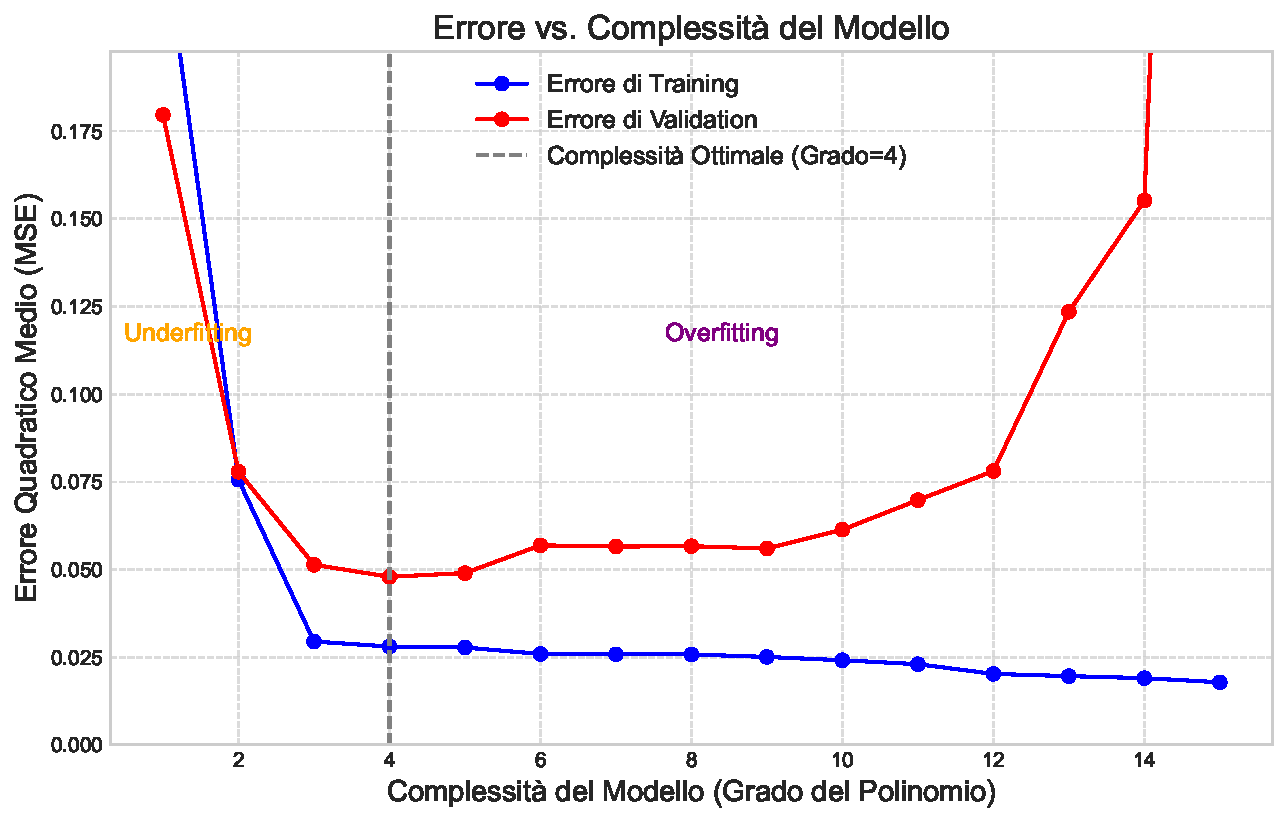
\includegraphics[width=0.7\textwidth]{images/error_vs_complexity.pdf}
    \caption{Andamento dell'errore sul training set e sul validation set al variare della complessità del modello.}
    \label{fig:error_vs_complexity}
\end{figure}

\begin{figure}[H]
    \centering
    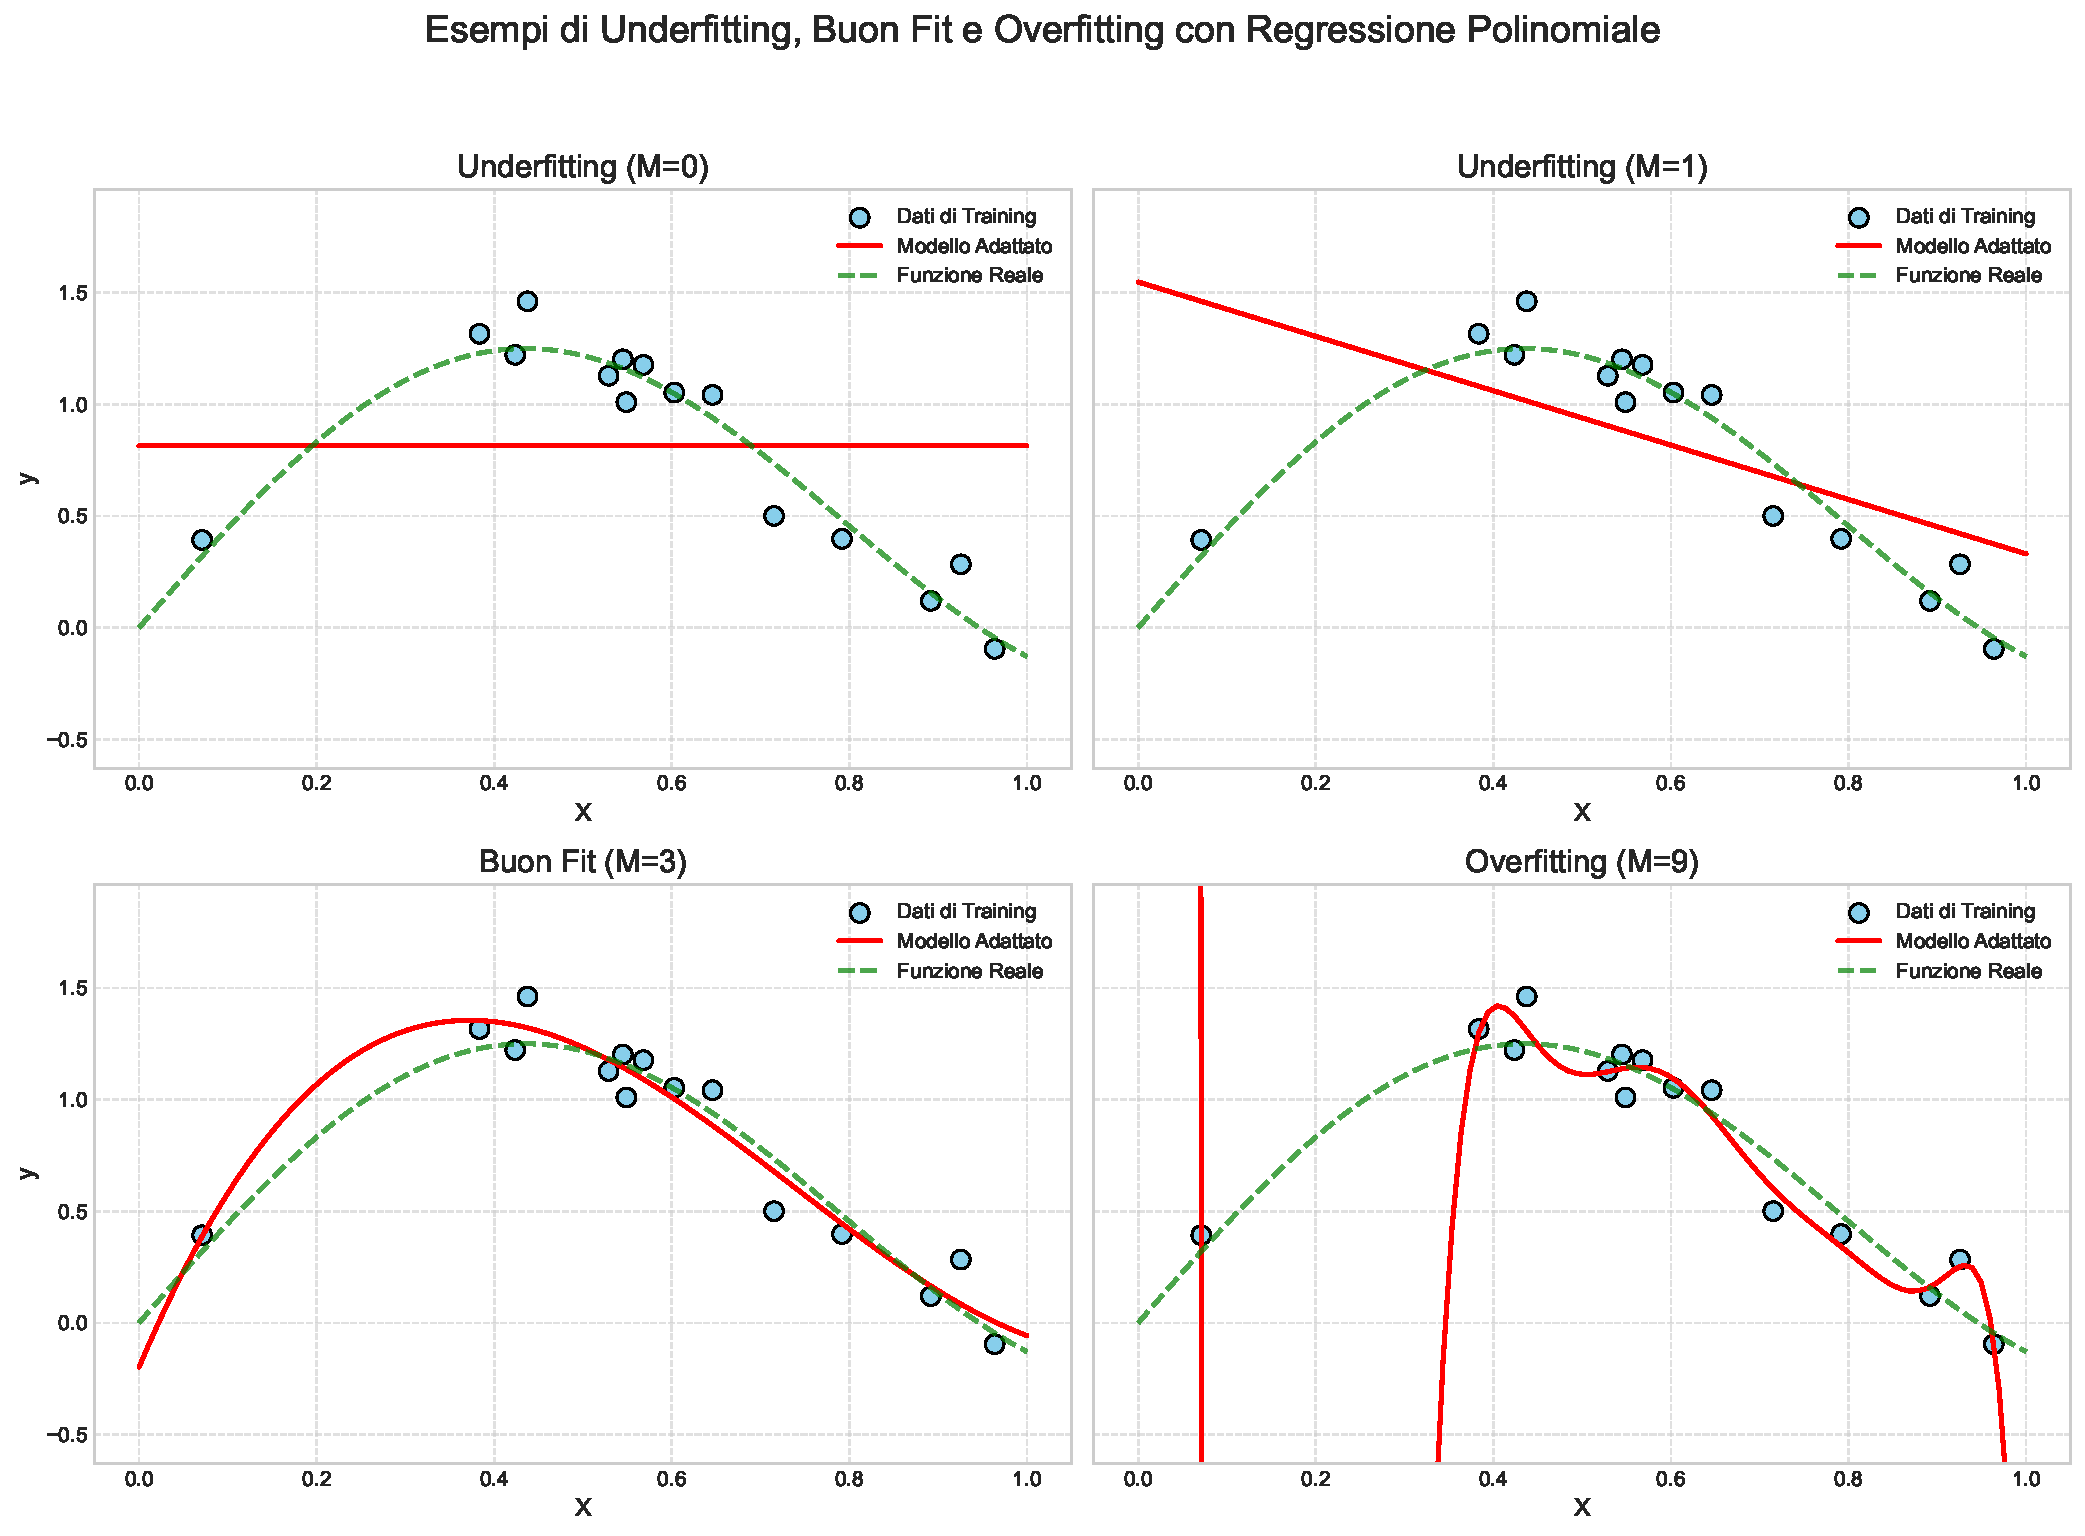
\includegraphics[width=\textwidth]{images/under_over_fitting.pdf}
    \caption{Esempi di underfitting (M=0, M=1), buon fit (M=3) e overfitting (M=9) con regressione polinomiale.}
    \label{fig:under_over_fitting}
\end{figure}

\subsection{Parametri e Iperparametri}
Nel processo di machine learning, è importante distinguere:
\begin{itemize}
    \item \textbf{Parametri del modello}: Sono i valori che il modello apprende dai dati durante il training. Ad esempio, i coefficienti $\theta_j$ in una regressione lineare o polinomiale.
    \item \textbf{Iperparametri}: Sono le configurazioni dell'algoritmo di learning che vengono impostate prima del training e non vengono apprese direttamente dai dati. Si determinano tipicamente cercando la configurazione che offre le migliori prestazioni sul validation set. Esempi includono: il tipo di funzione di regressione (lineare, polinomiale), il grado del polinomio, il tasso di apprendimento ($\eta$) nella discesa del gradiente, l'eventuale uso e tipo di normalizzazione o regolarizzazione.
\end{itemize}

\subsection{K-Fold Cross Validation}
Per ottenere una stima più robusta delle prestazioni di un modello e per la selezione degli iperparametri, si utilizza spesso la k-fold cross validation.
Il processo è il seguente:
\begin{enumerate}
    \item I dati vengono suddivisi in $k$ sottoinsiemi disgiunti (chiamati "fold").
    \item Si ripete il processo di addestramento e validazione $k$ volte. Ad ogni iterazione $j=1, \dots, k$:
          \begin{itemize}
              \item Il $j$-esimo fold viene usato come validation set.
              \item Gli altri $k-1$ fold vengono usati come training set per addestrare il modello.
          \end{itemize}
    \item Si ottengono $k$ modelli e $k$ stime di accuratezza (una per ogni fold di validazione).
    \item L'accuratezza finale del modello (o della configurazione di iperparametri) è la media delle $k$ accuratezze ottenute.
\end{enumerate}
Nella \textit{k-fold cross validation stratificata}, si cerca di mantenere in ogni fold una distribuzione delle classi (o delle caratteristiche dei dati) simile a quella del dataset completo.

\begin{figure}[H]
    \centering
    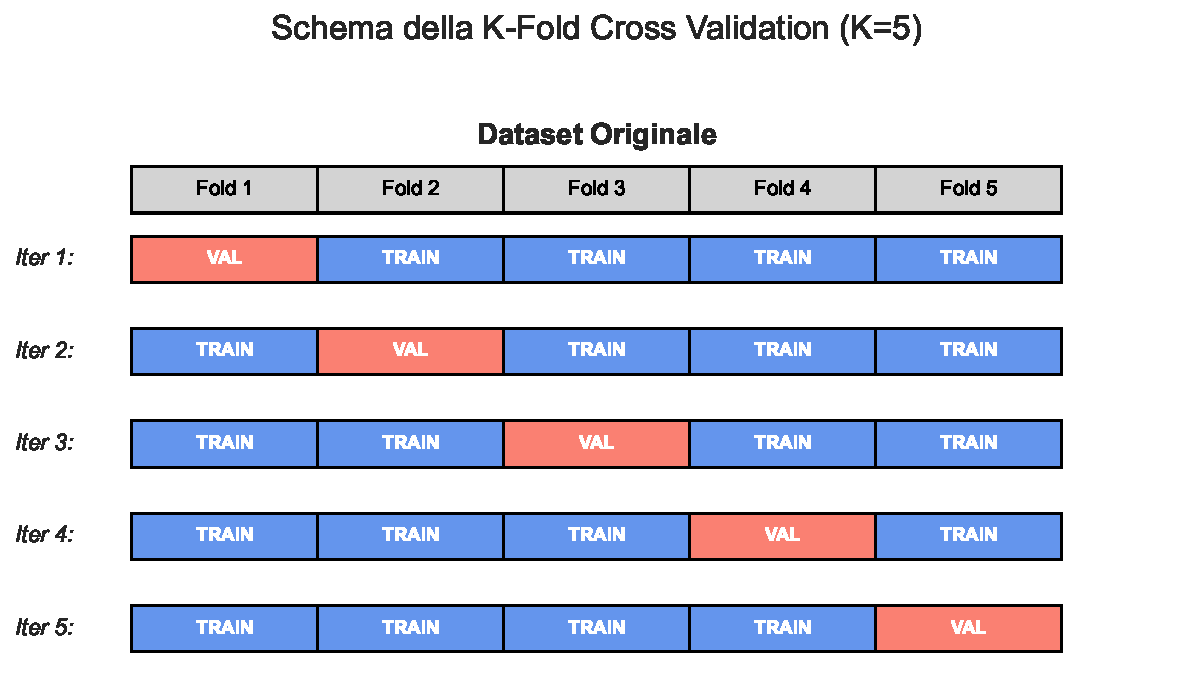
\includegraphics[width=0.8\textwidth]{images/k_fold_cross_validation.pdf}
    \caption{Schema della K-Fold Cross Validation.}
    \label{fig:k_fold_cv}
\end{figure}

\subsection{Regolarizzazione}
Quando si usano modelli complessi, come polinomi di grado elevato, i valori assoluti dei coefficienti $\theta_j$ possono diventare molto grandi. Questo può portare a forti oscillazioni nella funzione di regressione, rendendola instabile e peggiorando l'accuratezza su dati nuovi (overfitting).
La \textbf{regolarizzazione} è una tecnica utilizzata per contrastare l'overfitting, penalizzando i modelli con coefficienti di valore elevato. Si aggiunge un termine alla funzione d'errore MSE che dipende dalla magnitudine dei coefficienti:
$$ E_{\text{reg}}(\theta) = \text{MSE}(\theta) + \text{Termine di Penalizzazione}(\theta) $$
L'obiettivo diventa minimizzare questa nuova funzione d'errore.

\subsubsection{Ridge Regression (Regolarizzazione L2)}
La Ridge Regression aggiunge alla funzione d'errore un termine di penalizzazione proporzionale alla somma dei quadrati dei coefficienti (norma L2 al quadrato di $\theta$):
$$ \text{minimizza } \sum_{i=1}^{m} (\theta^T x^{(i)} - y^{(i)})^2 + \lambda ||\theta||_2^2 $$
dove $||\theta||_2^2 = \sum_{j=0}^{n} \theta_j^2$ (la somma include l'intercetta $\theta_0$ o talvolta la esclude dalla penalizzazione) e $\lambda \ge 0$ è l'iperparametro di regolarizzazione.
\begin{itemize}
    \item Se $\lambda = 0$, non c'è regolarizzazione e si ritorna all'MSE standard.
    \item All'aumentare di $\lambda$, la penalizzazione per coefficienti grandi aumenta, spingendo i loro valori a ridursi. Questo porta a modelli più "semplici" e meno inclini all'overfitting.
\end{itemize}
La soluzione analitica per $\theta$ nella Ridge Regression è (assumendo X includa la colonna di 1 per l'intercetta):
$$ \theta = (X^T X + \lambda I)^{-1} X^T y $$
dove $I$ è la matrice identità. È importante notare che, poiché la regolarizzazione L2 somma i quadrati dei coefficienti, la scala delle variabili di input può influenzare il risultato. Pertanto, è prassi comune \textbf{standardizzare} (o normalizzare) le variabili di input prima di applicare la Ridge Regression.

Geometricamente, la regolarizzazione L2 vincola la soluzione $\theta^*$ a trovarsi all'interno di un'ipersfera il cui raggio dipende da $\lambda$.

\begin{figure}[H]
    \centering
    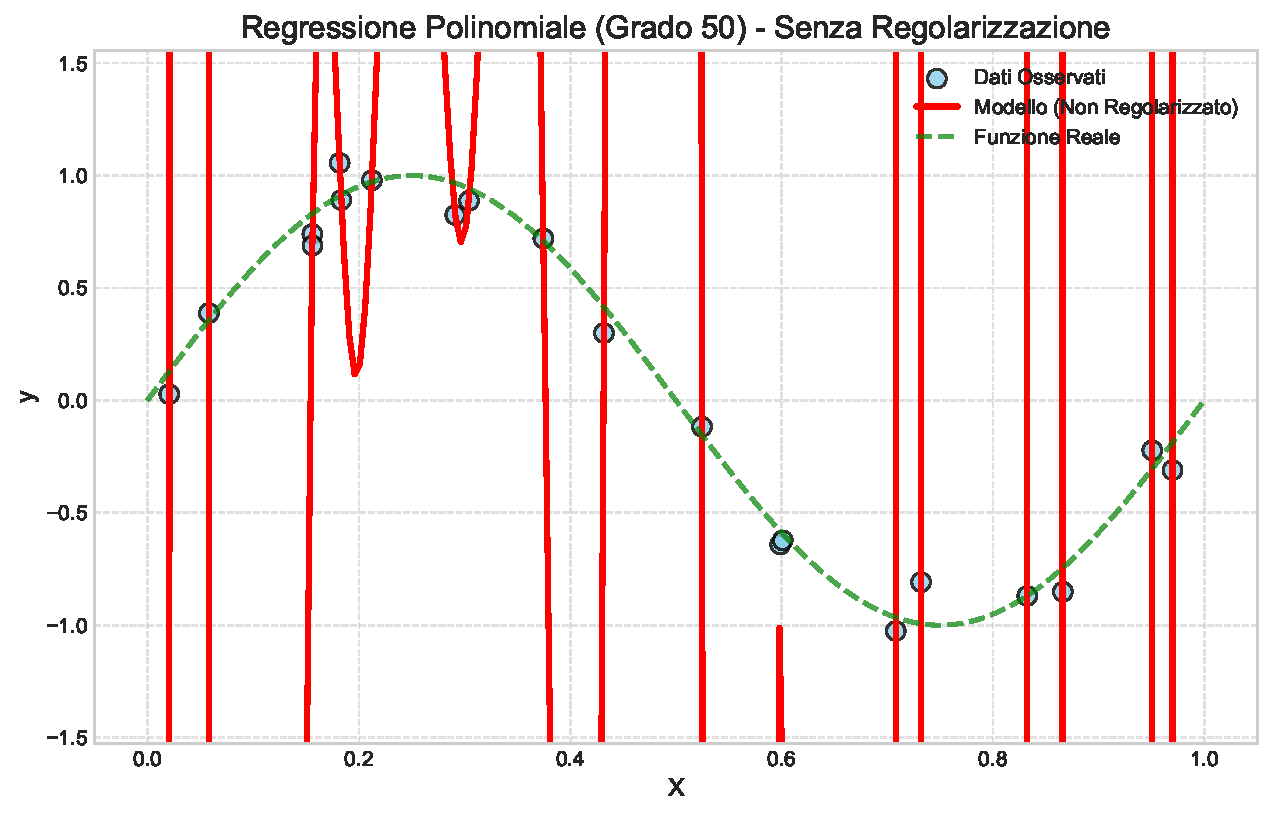
\includegraphics[width=0.7\textwidth]{images/poly50_no_reg.pdf}
    \caption{Regressione polinomiale di grado 50 senza regolarizzazione: possibili forti oscillazioni.}
    \label{fig:poly50_no_reg}
\end{figure}

\begin{figure}[H]
    \centering
    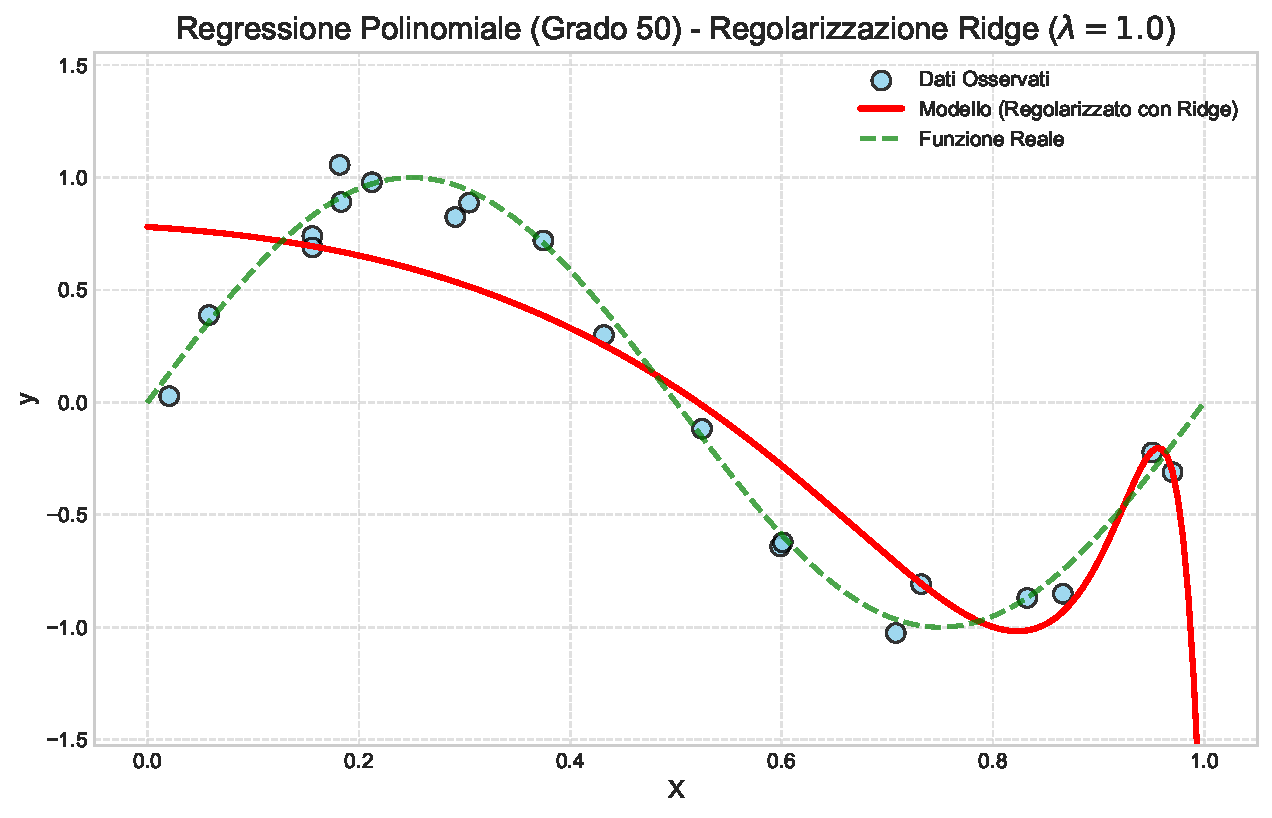
\includegraphics[width=0.7\textwidth]{images/poly50_with_reg.pdf}
    \caption{Regressione polinomiale di grado 50 con regolarizzazione Ridge ($\lambda=1$): oscillazioni ridotte.}
    \label{fig:poly50_with_reg}
\end{figure}

\subsubsection{LASSO Regression (Regolarizzazione L1)}
La regressione LASSO (Least Absolute Shrinkage and Selection Operator) utilizza la norma L1 per penalizzare i coefficienti:
$$ \text{minimizza } \sum_{i=1}^{m} (\theta^T x^{(i)} - y^{(i)})^2 + \lambda ||\theta||_1 $$
dove $||\theta||_1 = \sum_{j=0}^{n} |\theta_j|$.
A differenza della Ridge Regression che riduce i coefficienti verso lo zero ma raramente li azzera, la LASSO ha la proprietà di poter azzerare completamente alcuni coefficienti. Questo la rende utile anche per la \textbf{selezione delle feature}, in quanto le variabili i cui coefficienti vengono azzerati sono effettivamente escluse dal modello, portando a una soluzione "sparsa" e potenzialmente più interpretabile.
Geometricamente, la regolarizzazione L1 vincola la soluzione $\theta^*$ all'interno di un ipercubo (o politopo equivalente), e la soluzione ottimale tende a trovarsi sugli spigoli o vertici, dove alcune componenti di $\theta^*$ sono zero.

\begin{figure}[H]
    \centering
    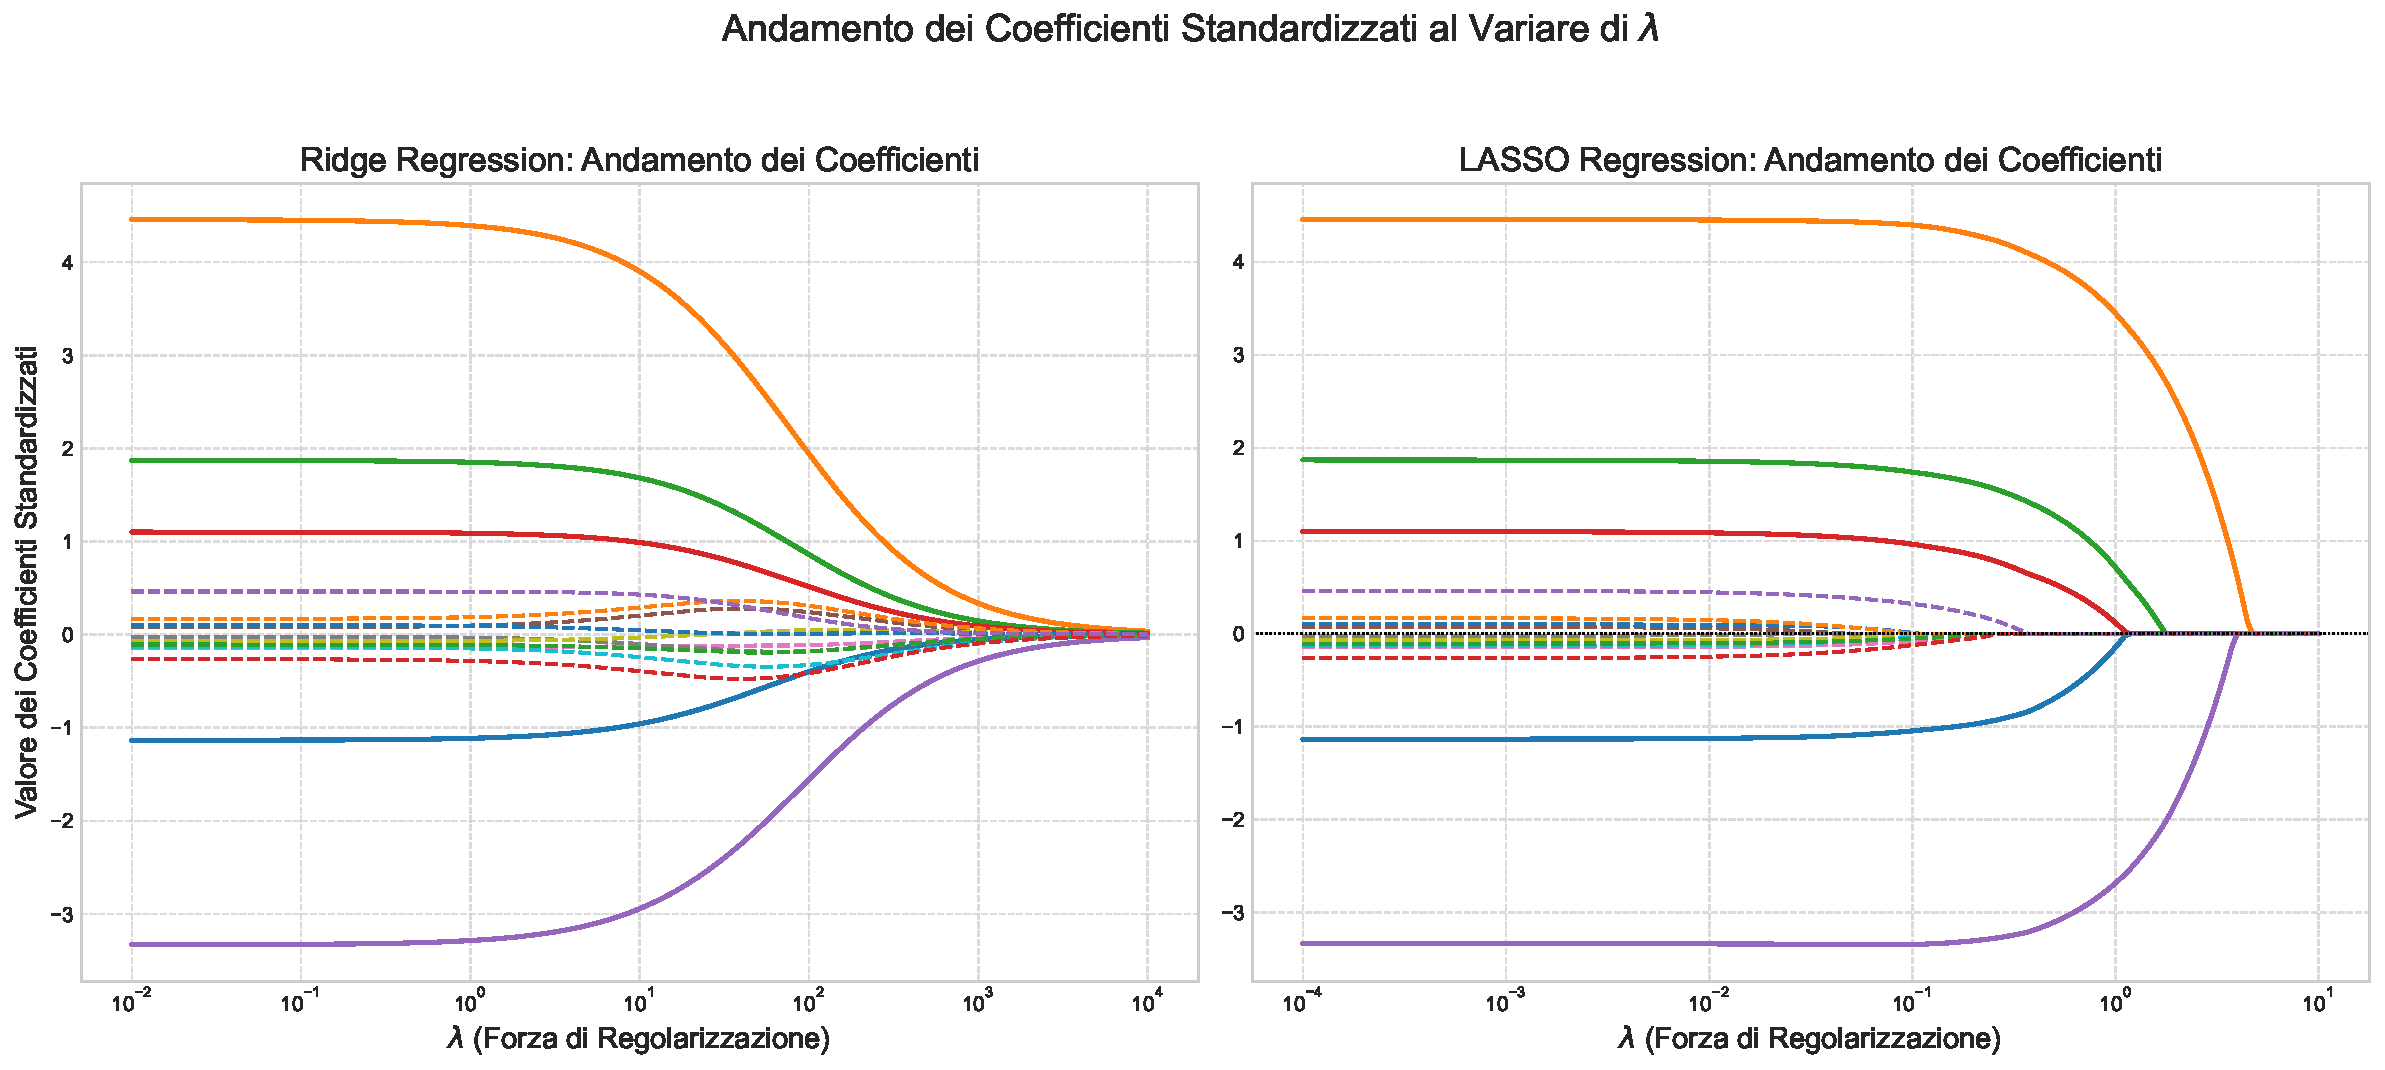
\includegraphics[width=\textwidth]{images/ridge_vs_lasso_coeffs.pdf}
    \caption{Andamento dei coefficienti standardizzati al variare di $\lambda$ per Ridge (sx) e LASSO (dx). LASSO tende ad azzerare i coefficienti delle variabili meno rilevanti.}
    \label{fig:ridge_vs_lasso_coeffs}
\end{figure}

\subsubsection{Elastic Net Regression (L1+L2)}
La regressione Elastic Net è una generalizzazione che combina entrambe le penalizzazioni L1 e L2:
$$ \text{minimizza } \sum_{i=1}^{m} (\theta^T x^{(i)} - y^{(i)})^2 + \lambda_1 ||\theta||_1 + \lambda_2 ||\theta||_2^2 $$
Spesso viene parametrizzata con un iperparametro $\alpha$ (da non confondere con il learning rate) che bilancia le due penalità, e un $\lambda$ complessivo:
$$ \text{minimizza } \sum_{i=1}^{m} (\theta^T x^{(i)} - y^{(i)})^2 + \lambda \left( \alpha ||\theta||_1 + (1-\alpha) ||\theta||_2^2 \right) $$
\begin{itemize}
    \item Con $\alpha=0$, si ha la Ridge Regression.
    \item Con $\alpha=1$, si ha la LASSO Regression.
    \item Valori di $\alpha$ intermedi combinano le proprietà di entrambe.
\end{itemize}

\subsubsection{Selezione degli Iperparametri (es. $\lambda$, grado del polinomio)}
La scelta ottimale degli iperparametri, come il grado del polinomio nella regressione polinomiale o il valore di $\lambda$ nella regolarizzazione, è cruciale. Questi vengono tipicamente scelti testando diverse combinazioni e selezionando quella che produce l'errore minore sul validation set, spesso utilizzando la k-fold cross validation.
Per una stima più affidabile delle prestazioni del modello finale e per evitare stime ottimistiche quando si ottimizzano molti iperparametri, si può ricorrere alla \textbf{Nested Cross Validation}. Questa tecnica prevede un ciclo di cross validation esterno per la valutazione del modello e un ciclo di cross validation interno, su ogni fold di training del ciclo esterno, per l'ottimizzazione degli iperparametri.

\subsection{Problema della Collinearità}
Nella regressione si assume generalmente che le variabili di input siano indipendenti tra loro. Se esistono forti dipendenze lineari tra due o più variabili di input (collinearità o multicollinearità), la stima dei coefficienti di regressione può diventare instabile: piccole variazioni nei dati di training possono generare modelli con coefficienti molto diversi, rendendo il modello inaffidabile e difficile da interpretare.
Ad esempio, se gli investimenti pubblicitari in TV e Radio sono fortemente correlati, potrebbe essere difficile isolare l'effetto individuale di ciascuno sulle vendite. La funzione d'errore potrebbe presentare una "valle" piatta, dove diverse combinazioni di coefficienti per TV e Radio producono un errore minimo simile, portando a soluzioni instabili.
Una soluzione è aggiungere termini di interazione nel modello (es. $\theta_k \cdot \text{TV} \cdot \text{Radio}$) se si sospetta un effetto sinergico. La regolarizzazione (Ridge, LASSO) può anche aiutare a mitigare i problemi di instabilità dovuti alla collinearità, poiché vincola le possibili soluzioni per i coefficienti.

\subsection{Esplosione della Dimensionalità e Funzioni Kernel}
Con la regressione polinomiale, il numero di termini (e quindi di parametri $\theta_j$) cresce rapidamente con il numero di variabili originali $n$ e il grado del polinomio $g$. Il numero di termini generati è $\binom{n+g}{g}$. Ad esempio, con 10 variabili e un polinomio di grado 10, si generano 184756 parametri, rendendo l'approccio non scalabile e problematico se il numero di variabili diventa comparabile o maggiore del numero di istanze (problema dell'elevata dimensionalità).

\subsubsection{Il "Kernel Trick"}
Le funzioni kernel offrono un modo per operare in uno spazio delle feature ad elevata (potenzialmente infinita) dimensionalità senza dover calcolare esplicitamente le coordinate dei dati in tale spazio. L'idea è che molti algoritmi (inclusa la Ridge Regression) richiedono solo i prodotti scalari tra i vettori delle feature. Se si può trovare una funzione kernel $K(x, z)$ che calcola il prodotto scalare $\phi(x)^T \phi(z)$ nello spazio trasformato $\phi$ direttamente dai dati originali $x, z$, allora non è necessario esplicitare la trasformazione $\phi(x)$.
Per un kernel polinomiale, ad esempio:
$$ K(x, z) = (x^T z + c)^g $$
calcolare $K(x,z)$ è molto meno costoso che calcolare prima $\phi(x)$ e $\phi(z)$ (che avrebbero $\binom{n+g}{g}$ componenti) e poi il loro prodotto scalare.

\subsubsection{Regressione con Kernel (Kernel Ridge Regression)}
Nella regressione, si può dimostrare che i coefficienti ottimali $\theta^*$ possono essere espressi come una combinazione lineare delle istanze di training trasformate: $\theta^* = \sum_{i=1}^{m} \alpha_i \phi(x^{(i)})$. Sostituendo questa espressione nella funzione obiettivo della Ridge Regression e utilizzando il kernel trick, si arriva a una formulazione in cui si devono apprendere i coefficienti $\alpha_i$ (uno per ogni istanza di training) invece dei $\theta_j$.
La funzione d'errore da minimizzare rispetto ad $\alpha$ diventa:
$$ \text{minimizza } \frac{1}{m} ||K\alpha - y||_2^2 + \lambda \alpha^T K \alpha $$
dove $K$ è la matrice kernel $m \times m$ tale che $K_{ij} = K(x^{(i)}, x^{(j)})$, e $\alpha = [\alpha_1, \dots, \alpha_m]^T$.
La soluzione per $\alpha$ è:
$$ \alpha = (K + \lambda m I)^{-1} y $$
Questa è nota come \textbf{Kernel Ridge Regression}. Permette di ottenere gli stessi risultati di una regressione polinomiale di grado elevato (o con altre trasformazioni complesse) senza creare esplicitamente le feature aggiuntive, mitigando l'esplosione della dimensionalità.

\subsubsection{Altre Funzioni Kernel}
Oltre al kernel polinomiale, esistono altre funzioni kernel popolari:
\begin{itemize}
    \item \textbf{Gaussian Radial Basis Function (RBF) Kernel}: $K(x, z) = e^{\left(-\gamma ||x-z||^2\right)}$ con $\gamma = \frac{1}{2\sigma^2}$. Questo kernel mappa i dati in uno spazio a infinite dimensioni e può modellare relazioni molto complesse.
    \item \textbf{Kernel Sigmoidale}: $K(x, z) = \tanh(k x^T z - \delta)$.
\end{itemize}
La scelta del kernel e dei suoi iperparametri (es. $g, c$ per il polinomiale; $\gamma$ per RBF) è cruciale e viene solitamente fatta tramite cross-validation.

% Fine file 06_Aula_Previsione_con_Regressione_non_lineare.pdf



\section{Sistemi di Raccomandazione (Recommendation Systems)}


\subsection{Introduzione e Motivazioni}
I Sistemi di Raccomandazione (Recommender Systems - RS) sono strumenti software e tecniche che mirano a fornire suggerimenti personalizzati ("raccomandazioni") agli utenti su item (prodotti, servizi, informazioni, ecc.) che potrebbero trovare interessanti o utili.

\begin{examplebox}{Un Esempio Pratico: La Previsione di Target}
    Una nota storia illustra il potenziale dei sistemi di analisi predittiva, simili concettualmente ai motori di raccomandazione. Nel marzo 2012, un padre si lamentò con la catena di supermercati Target perché la figlia adolescente riceveva coupon per prodotti per la maternità. Il manager si scusò per l'errore, ma alcuni giorni dopo fu il padre a scusarsi: dopo aver parlato con la figlia, aveva scoperto che lei era effettivamente incinta e avrebbe partorito in agosto.
    Target era riuscita a prevedere la gravidanza analizzando lo storico degli acquisti associati a un codice cliente. Ad esempio, l'analisi dei dati aveva rivelato che le donne incinte tendono ad acquistare più lozioni inodore all'inizio del secondo trimestre e specifici integratori. Identificando circa 25 prodotti, Target poteva stimare la fase della gravidanza e persino una finestra per la data di nascita, inviando coupon mirati. Curiosamente, Target scoprì anche che pubblicità troppo focalizzate sulla maternità potevano essere percepite come invadenti; mescolare coupon per la maternità con offerte generiche risultava più efficace. Questo caso evidenzia come l'analisi dei dati possa portare a previsioni molto specifiche sul comportamento e le esigenze future degli utenti.
\end{examplebox}

\subsubsection{Perché Utilizzare i Sistemi di Raccomandazione?}
I sistemi di raccomandazione offrono valore sia ai clienti che ai fornitori di servizi/prodotti.

\begin{itemize}
    \item \textbf{Valore per il Cliente}:
          \begin{itemize}
              \item Trovare item rilevanti rispetto ai propri interessi, spesso superando il sovraccarico informativo.
              \item Migliorare ed espandere l'insieme delle scelte possibili.
              \item Aiutare ad esplorare lo spazio delle opzioni disponibili.
              \item Fornire intrattenimento e scoperta.
          \end{itemize}
    \item \textbf{Valore per il Provider}:
          \begin{itemize}
              \item Offrire un servizio personalizzato aggiuntivo per i clienti.
              \item Aumentare la fiducia e la fidelizzazione dei clienti.
              \item Incrementare le vendite, ad esempio attraverso un aumento dei click-through rates (CTR) sugli oggetti proposti.
              \item Opportunità per promozione mirata e persuasione.
              \item Ottenere maggiore conoscenza sui clienti analizzando il loro gradimento delle proposte fatte.
          \end{itemize}
\end{itemize}
Grandi aziende come Amazon.com e Netflix attribuiscono una porzione significativa delle loro vendite (tra il 30\% e il 70\%) ai loro sistemi di raccomandazione. Altri esempi includono LinkedIn (raccomandazione di gruppi, persone, posti di lavoro), Facebook (amici, pubblicità personalizzate), Spotify/Last.fm (canzoni) e Forbes.com (notizie, con un aumento del 37\% del CTR grazie al recommender).

\begin{notebox}{Il Contesto del Netflix Grand Prize}
    L'importanza dei sistemi di raccomandazione è stata sottolineata dal "Netflix Grand Prize Contest". Netflix offrì un premio di 1 milione di dollari al team che fosse riuscito a migliorare di almeno il 10\% la capacità predittiva del proprio sistema di raccomandazione di film (misurata tramite la radice dell'errore quadratico medio - RMSE). Il dataset di training conteneva oltre 100 milioni di valutazioni (scala 1-5) da circa 480.000 utenti su quasi 18.000 film.
\end{notebox}

\subsubsection{Il Fenomeno della "Long Tail"}
Nella vendita online, il numero di prodotti disponibili è vastissimo, molto superiore a quanto un utente possa analizzare singolarmente. I sistemi di raccomandazione aiutano a navigare questa abbondanza, individuando i prodotti con maggiore propensione di acquisto per un utente specifico. Questo contrasta con il mondo fisico, dove i prodotti esposti sono generalmente di meno (spesso solo i più popolari) e l'utente può esaminarli quasi tutti.
Si osserva il fenomeno della "long tail" (coda lunga): pochi prodotti (la "testa") sono acquistati o visionati moltissimo, mentre la stragrande maggioranza dei prodotti (la "coda") riceve poche interazioni individuali, ma collettivamente può rappresentare una quota di mercato significativa. Ad esempio, su MovieLens, il 74\% delle valutazioni positive riguardava solo il 20\% dei prodotti disponibili. I RS possono aiutare a scoprire e valorizzare i prodotti nella coda lunga.

\begin{figure}[H]
    \centering
    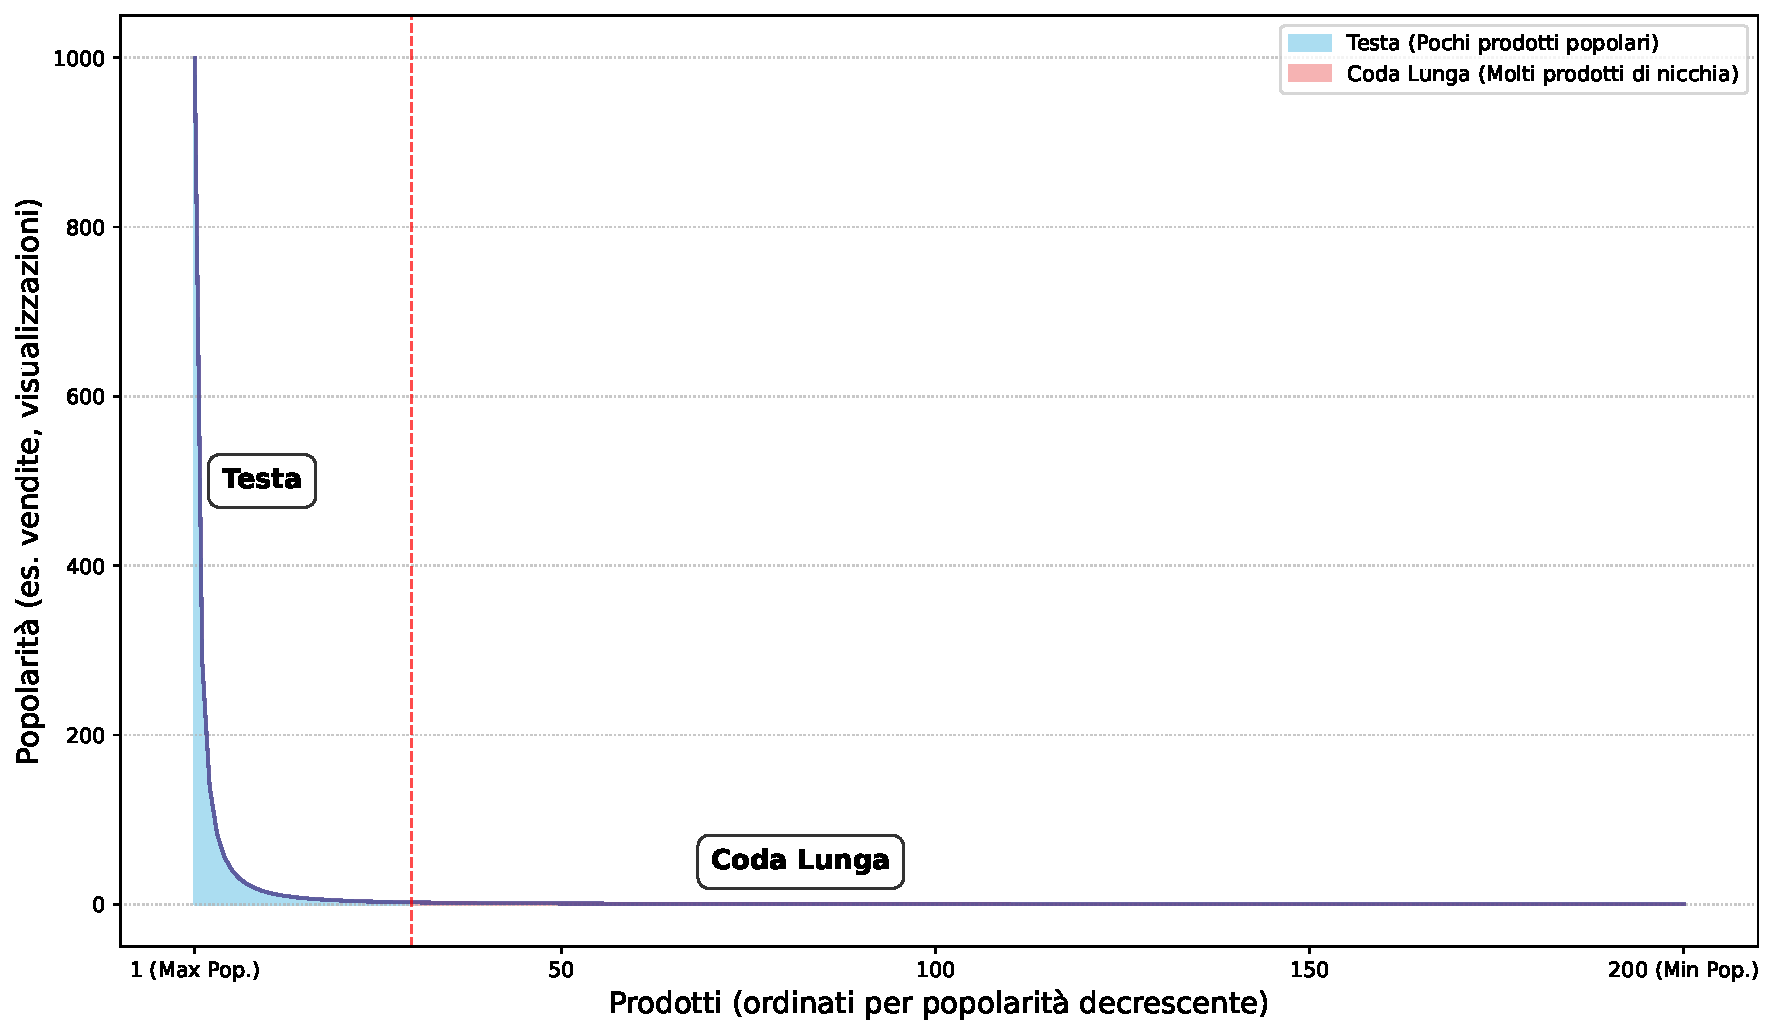
\includegraphics[width=1\textwidth]{images/long_tail_graph.pdf}
    \caption{Illustrazione del fenomeno della Long Tail: popolarità dei prodotti.}
    \label{fig:long_tail}
\end{figure}

\subsection{Concetti Fondamentali}

\subsubsection{La Matrice di Utilità (Utility Matrix)}
Nei sistemi di raccomandazione, gli attori principali sono gli utenti e gli item (prodotti, notizie, film, ecc.). I dati sulle interazioni tra utenti e item sono tipicamente organizzati in una \textbf{matrice di utilità} (o matrice di rating):
\begin{itemize}
    \item Ogni riga corrisponde a un utente.
    \item Ogni colonna corrisponde a un item.
    \item Ogni cella $(u, i)$ contiene la valutazione (rating) data dall'utente $u$ all'item $i$. La cella può essere vuota se l'utente non ha valutato l'item.
\end{itemize}
La matrice può essere:
\begin{itemize}
    \item \textbf{Binaria}: Indica se l'utente ha interagito (es. acquistato, cliccato = 1) o meno (= 0) con un item.
    \item \textbf{Discreta}: Contiene valutazioni su una scala (es. da 1 a 5 stelle).
\end{itemize}
Una caratteristica fondamentale della matrice di utilità è la sua \textbf{sparsità}: ogni utente interagisce o valuta solo una piccolissima frazione del totale degli item disponibili.

\begin{figure}[H]
    \centering
    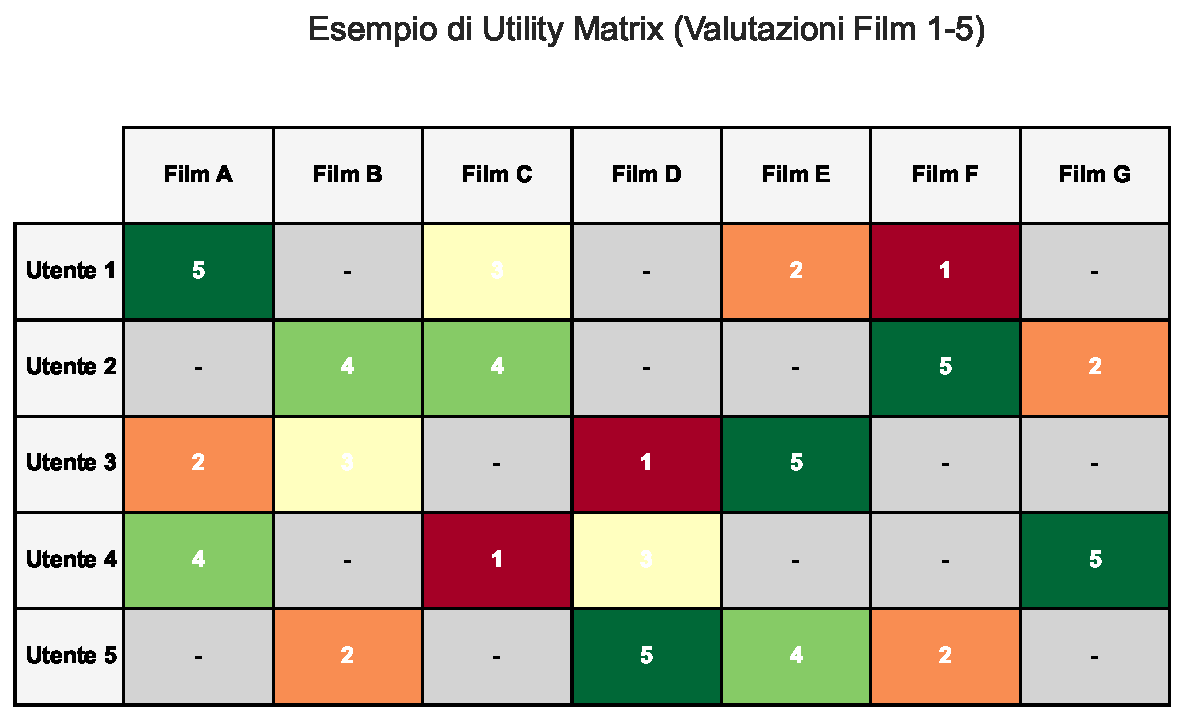
\includegraphics[width=0.7\textwidth]{images/utility_matrix_example.pdf}
    \caption{Esempio di Utility Matrix con valutazioni di film (scala 1-5). Le celle vuote indicano film non valutati.}
    \label{fig:utility_matrix_example}
\end{figure}

\subsubsection{Tipi di Giudizi (Feedback)}
Le valutazioni o interazioni possono essere di due tipi principali:

\begin{definitionbox}{Giudizi Espliciti}
    Sono feedback diretti e intenzionali forniti dagli utenti, e rappresentano con maggiore probabilità un'indicazione precisa della loro preferenza. Sono i più comunemente utilizzati e possono essere su scale numeriche (es. 1-5 stelle) o binarie (es. "mi piace / non mi piace").
    \textbf{Aspetti di studio} includono la granularità ottimale della scala (es. per i film, una scala 0-10 si è dimostrata efficace) e le valutazioni multidimensionali (es. voti separati per attori, colonna sonora di un film).
    \textbf{Problemi principali}:
    \begin{itemize}
        \item Gli utenti non sono sempre disposti a votare molti prodotti.
        \item Il numero di voti espliciti disponibili potrebbe essere troppo piccolo, portando a una matrice di utilità molto sparsa e di scarsa qualità per le predizioni.
        \item Come incentivare gli utenti a valutare più item è una sfida aperta.
    \end{itemize}
\end{definitionbox}

\begin{definitionbox}{Giudizi Impliciti}
    Sono feedback raccolti indirettamente dal comportamento dell'utente durante l'interazione con un sistema (es. negozio web, applicazione). Non richiedono uno sforzo esplicito da parte dell'utente. Esempi includono:
    \begin{itemize}
        \item Acquisto di un prodotto (considerato spesso una valutazione positiva, anche se non sempre vero).
        \item Click su un link, visualizzazioni di pagine, tempo speso su una pagina, download di demo.
    \end{itemize}
    Possono essere raccolti costantemente e in grande quantità.
    \textbf{Problema principale}: Non si può essere certi che il comportamento dell'utente sia interpretato correttamente. Ad esempio, un utente potrebbe non gradire tutti i libri che compra, o potrebbe averli comprati per qualcun altro.
    Spesso si utilizzano giudizi impliciti insieme a quelli espliciti, a volte chiedendo conferma all'utente sull'interpretazione del suo comportamento.
\end{definitionbox}


\subsection{Principali Approcci ai Sistemi di Raccomandazione}
Esistono diverse macro-famiglie di approcci per la costruzione di sistemi di raccomandazione:
\begin{itemize}
    \item \textbf{Sistemi Collaborativi (Collaborative Filtering)}: Si basano sul principio "Dimmi ciò che è popolare tra gli utenti con interessi simili ai miei". Analizzano i comportamenti e le preferenze di un'ampia comunità di utenti.
    \item \textbf{Sistemi Basati sul Contenuto (Content-based)}: L'idea è "Mostrami oggetti simili per contenuto a ciò che ho apprezzato in passato". Questi sistemi raccomandano item analizzando le loro caratteristiche e confrontandole con il profilo di interesse dell'utente, derivato dagli item che l'utente ha gradito in precedenza. Ad esempio, individuano libri simili per genere, autore o trama a quelli già letti e apprezzati.
    \item \textbf{Sistemi Basati sulla Conoscenza (Knowledge-based)}: Operano secondo il principio "Dimmi quello che si adatta a me in base alle mie esigenze specifiche". L'utente esprime esplicitamente le caratteristiche del prodotto di interesse (es. tramite un form o un questionario), e il sistema cerca i prodotti che meglio soddisfano tali requisiti.
    \item \textbf{Sistemi Ibridi}: Combinano tecniche provenienti da due o più degli approcci precedenti per sfruttarne i rispettivi punti di forza e mitigarne le debolezze.
\end{itemize}

\subsection{Collaborative Filtering (CF)}
Il Collaborative Filtering (CF) raggruppa un insieme di approcci che sono generalmente i più utilizzati nei sistemi di raccomandazione, impiegati da grandi siti di e-commerce e applicabili in vari settori (libri, film, news, ecc.).
Il \textbf{razionale} alla base è utilizzare la "saggezza della massa" (wisdom of the crowd) per formulare raccomandazioni.
L'\textbf{assunzione di base} è che siano disponibili i voti (giudizi espliciti o impliciti) degli utenti per gli articoli del catalogo.
L'\textbf{ipotesi fondamentale} è: se gli utenti hanno avuto interessi simili in passato, avranno interessi simili anche in futuro.

\subsubsection{Approcci Classici al Collaborative Filtering}
\begin{itemize}
    \item \textbf{Input}: La matrice di utilità (rating Utenti-Prodotti).
    \item \textbf{Output}:
          \begin{itemize}
              \item Una previsione di quanto l'utente gradirà o meno un determinato prodotto non ancora valutato.
              \item Un elenco ordinato dei top-N item consigliati per l'utente.
          \end{itemize}
\end{itemize}
Si distinguono principalmente due approcci:
\begin{itemize}
    \item \textbf{Memory-based}: Utilizzano direttamente i dati grezzi (gusti, voti, click, ecc.) per rilevare correlazioni tra utenti o tra item e raccomandare a un utente $u$ un oggetto $p$ che non ha precedentemente valutato o acquistato.
    \item \textbf{Model-based}: L'obiettivo è il medesimo, ma questi approcci utilizzano algoritmi di apprendimento automatico per costruire modelli predittivi (modelli di learning) basati sui dati storici. Questi modelli vengono poi usati per fare raccomandazioni a ogni utente.
\end{itemize}

\subsubsection{User-based Nearest-Neighbor CF (CF Basato su Utenti Simili)}
Questo è un approccio memory-based. Considerato un utente attivo (es. Carl), per predire il suo gradimento per un prodotto $p$ che non ha ancora valutato/comprato, l'algoritmo procede come segue:
\begin{enumerate}
    \item Trovare il set di utenti (vicini, "neighbors") più simili all'utente attivo, basandosi sui voti che hanno espresso sugli stessi prodotti. Questi utenti simili devono aver valutato il prodotto $p$.
    \item Utilizzare i voti assegnati da questo set di utenti simili al prodotto $p$ per predire il voto dell'utente attivo per $p$ (ad esempio, usando una media pesata dei voti).
    \item Ripetere questa operazione per tutti i prodotti non ancora valutati dall'utente attivo e raccomandare quelli con il voto predetto più alto.
\end{enumerate}

\begin{figure}[H]
    \centering
    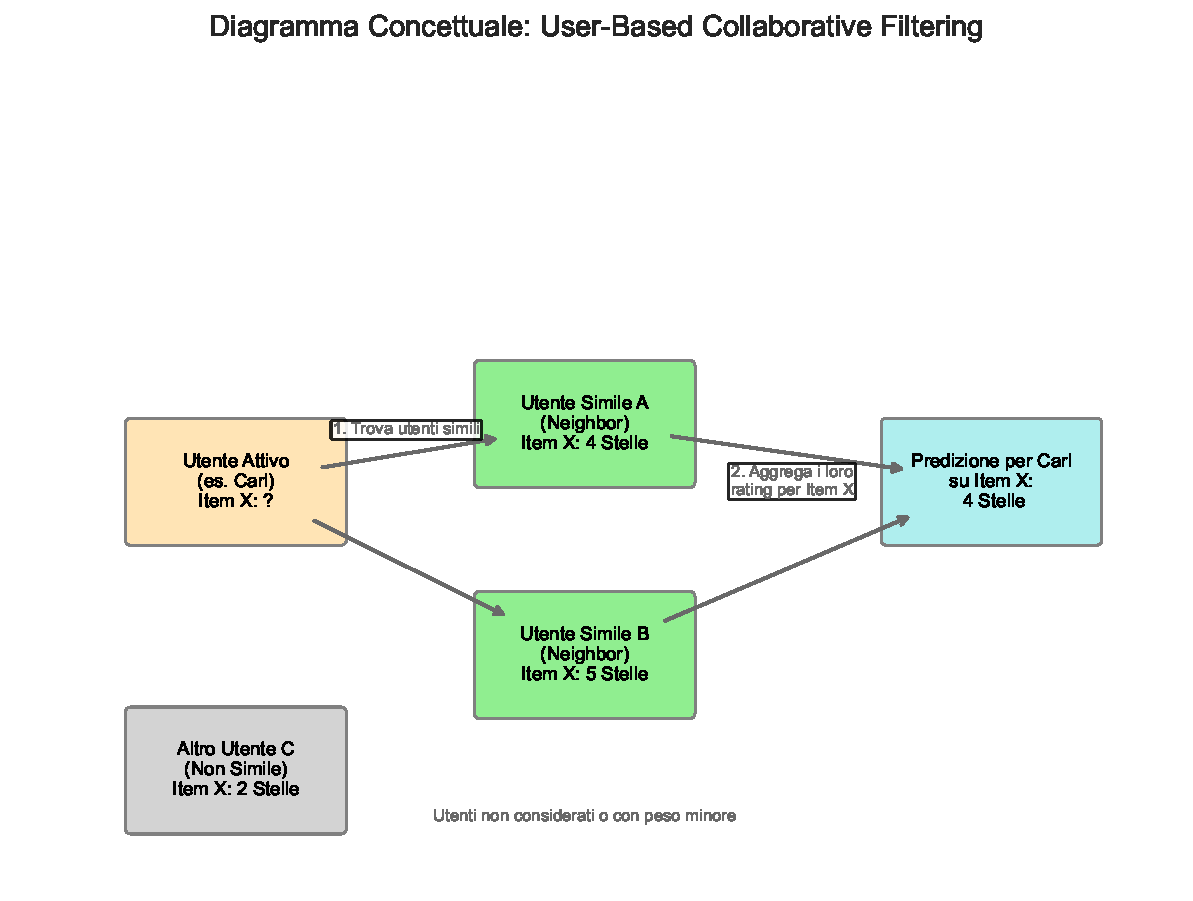
\includegraphics[width=0.8\textwidth]{images/user_based_cf_diagram.pdf} 
    \caption{Diagramma concettuale del Collaborative Filtering User-based.}
    \label{fig:user_based_cf}
\end{figure}

L'\textbf{ipotesi} è che se gli utenti hanno votato/acquistato in maniera simile in passato, lo faranno anche in futuro. Le preferenze degli utenti sono considerate relativamente stabili nel tempo.

Per implementare questo approccio, bisogna definire:
\begin{itemize}
    \item Come misurare la similarità tra utenti?
    \item Quanti utenti simili (vicini) considerare?
    \item Come generare una previsione partendo dai rating degli utenti considerati?
\end{itemize}

\paragraph{Misure di Similarità tra Utenti.}
Siano $a$ e $b$ due utenti, e $P$ l'insieme dei prodotti per cui sia $a$ che $b$ hanno espresso un giudizio. Siano $r_{a,p}$ e $r_{b,p}$ i rating rispettivi.

\begin{definitionbox}{Correlazione di Pearson}
    Misura la correlazione lineare tra i rating dei due utenti sugli item in comune. Siano $\overline{r}_a$ e $\overline{r}_b$ i valori medi dei giudizi degli utenti $a$ e $b$ per i prodotti in $P$.
    $$ \text{sim\_pearson}(a,b) = \frac{\sum_{p \in P} (r_{a,p} - \overline{r}_a) (r_{b,p} - \overline{r}_b)}{\sqrt{\sum_{p \in P} (r_{a,p} - \overline{r}_a)^2} \sqrt{\sum_{p \in P} (r_{b,p} - \overline{r}_b)^2}} $$
    Il risultato è compreso tra -1 e 1:
    \begin{itemize}
        \item $>0$: correlazione positiva.
        \item $=0$: nessuna correlazione lineare.
        \item $<0$: correlazione inversa (gli utenti hanno gusti opposti).
    \end{itemize}
    Questa è la misura più utilizzata. Per correlazioni non lineari o variabili non gaussiane, si può usare la correlazione di Spearman.
\end{definitionbox}

\begin{definitionbox}{Similarità Coseno}
    Considera i rating di ciascun utente sugli item in comune $P$ come vettori ($r_a$, $r_b$) e calcola il coseno dell'angolo tra di essi.
    $$ \text{sim\_cosine}(a,b) = \frac{\sum_{p \in P} (r_{a,p} \cdot r_{b,p})}{\sqrt{\sum_{p \in P} (r_{a,p})^2} \sqrt{\sum_{p \in P} (r_{b,p})^2}} = \frac{r_a \cdot r_b}{||r_a|| \cdot ||r_b||} $$
    I valori sono compresi tra 0 (massima dissimilarità, vettori ortogonali) e 1 (massima similarità, vettori con stessa direzione). Altre misure includono la distanza di Jaccard.
\end{definitionbox}

\paragraph{Generare una Predizione per l'Utente Attivo.}
Sia $a$ l'utente attivo, $p$ il prodotto da predire, $N$ l'insieme degli utenti più simili ad $a$ che hanno valutato $p$, e $\overline{r}_a$ la media dei giudizi espressi da $a$. La predizione $pred(a,p)$ può essere calcolata come:
$$ pred(a,p) = \overline{r}_a + \frac{\sum_{b \in N} \text{sim}(a,b) \cdot (r_{b,p} - \overline{r}_b)}{\sum_{b \in N} |\text{sim}(a,b)|} $$
dove $\text{sim}(a,b)$ è la similarità tra $a$ e $b$, e $(r_{b,p} - \overline{r}_b)$ è la differenza tra il giudizio dell'utente $b$ su $p$ e il giudizio medio di $b$ sui prodotti in comune con $a$ (o su tutti i prodotti valutati da $b$). La similarità $\text{sim}(a,b)$ funge da peso.

\paragraph{Miglioramenti nelle Predizioni User-based.}
Per migliorare la qualità delle predizioni si possono adottare diverse strategie:
\begin{itemize}
    \item Dare maggior peso agli accordi su item "controversi" (con alta varianza nei voti) rispetto a item universalmente apprezzati.
    \item Considerare l'importanza del numero di item valutati in comune (co-rated items), ad esempio riducendo il peso della similarità se il numero di item co-valutati è basso.
    \item Amplificare il peso degli utenti "molto simili" (con similarità vicina a 1).
    \item Selezionare il numero di vicini $N$ tramite una soglia di similarità o un numero fisso.
\end{itemize}

\subsubsection{Item-based Nearest-Neighbor CF (CF Basato su Item Simili)}
Questo approccio, spesso considerato model-based (dove il "modello" è la matrice di similarità item-item precalcolata) o talvolta memory-based, utilizza la similarità tra prodotti (e non tra utenti) per fare previsioni.
\textbf{Idea di base}: Per predire il voto dell'utente Carl per item5, si individuano gli item (es. item1, item4) che Carl ha già valutato e che sono più simili a item5. Si utilizzano quindi i giudizi di Carl su item1 e item4 per stimare quello per item5.


\begin{figure}[H]
    \centering
    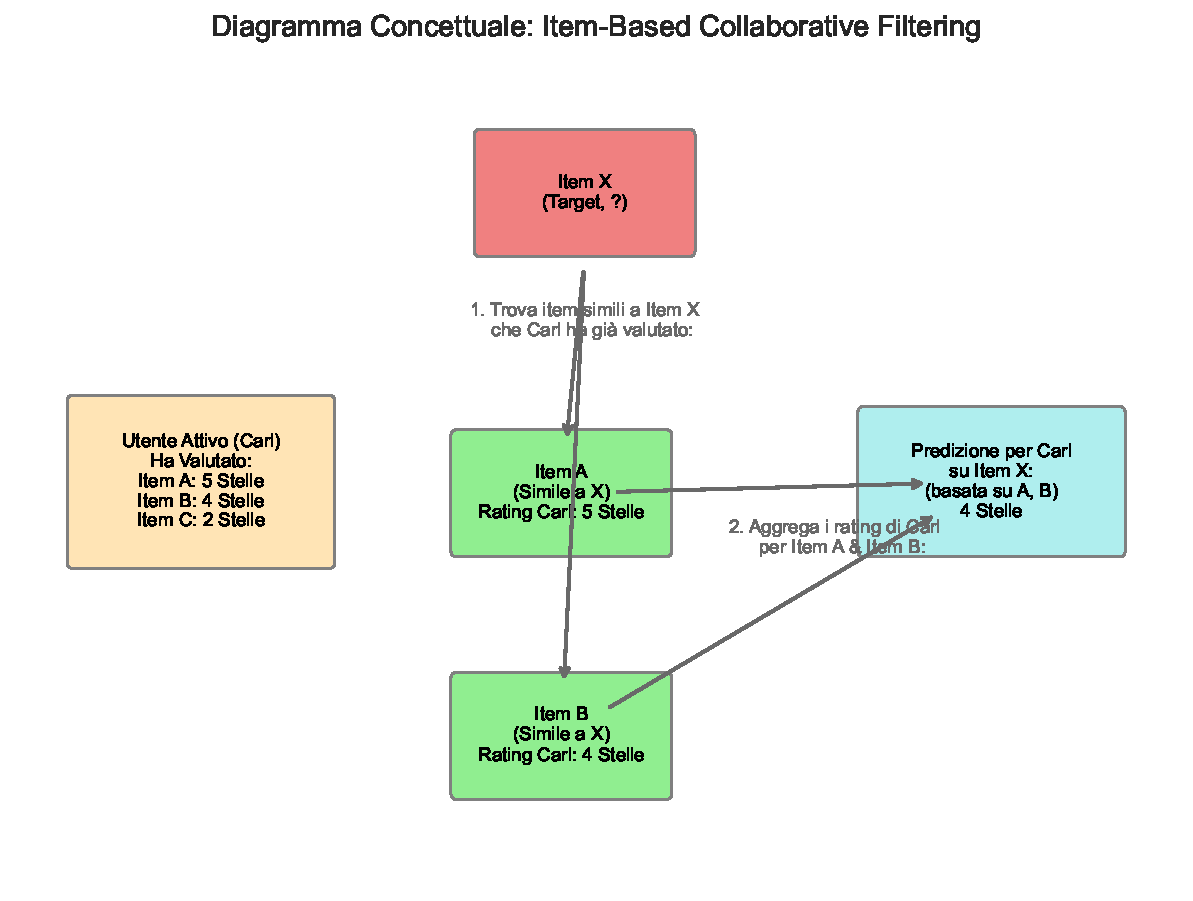
\includegraphics[width=0.8\textwidth]{images/item_based_cf_diagram.pdf}
    \caption{Diagramma concettuale del Collaborative Filtering Item-based.}
    \label{fig:item_based_cf}
\end{figure}

\paragraph{Parametri e Similarità Item-Item.}
\begin{itemize}
    \item \textbf{Similarità tra Item}: La similarità coseno tra i vettori dei rating ricevuti da due item (cioè, le colonne della utility matrix) è spesso la più efficace. Una variante consiste nell'aggiustare i rating sottraendo la media dei voti di ciascun utente prima di calcolare la similarità.
    \item \textbf{Dimensione del Vicinato}: Il numero di item simili da considerare è in genere fisso e relativamente piccolo (es. 20-50 item simili).
\end{itemize}

\paragraph{Formula di Predizione Item-based.}
Sia $u$ l'utente, $p$ il prodotto target, $r_{u,i}$ il rating dato dall'utente $u$ all'item $i$, e $\text{ratedItems}(u)$ l'insieme degli item valutati da $u$ che sono simili a $p$. La predizione $pred(u,p)$ può essere calcolata come una media pesata dei rating dati da $u$ agli item simili a $p$:
$$ pred(u,p) = \frac{\sum_{i \in \text{ratedItems}(u) \cap \text{similarItems}(p)} \text{sim}(i,p) \cdot r_{u,i}}{\sum_{i \in \text{ratedItems}(u) \cap \text{similarItems}(p)} |\text{sim}(i,p)|} $$

\paragraph{Pre-processing per l'Approccio Item-based.}
Per migliorare la scalabilità, le similarità tra tutte le coppie di item possono essere calcolate offline (pre-processing). Questo perché le similarità tra item tendono ad essere più stabili nel tempo rispetto a quelle tra utenti.
La memorizzazione di $N^2$ similarità (con $N$ numero di item) può essere un problema, ma in pratica il numero è minore perché si considerano solo item con un numero minimo di co-rating (utenti che li hanno valutati entrambi). Si può anche limitare a priori la dimensione del set di item simili.

\subsubsection{Sfide Comuni del Collaborative Filtering}

\begin{definitionbox}{Cold Start e Sparsità dei Dati}
    Il problema del "cold start" si verifica quando si devono fare raccomandazioni per nuovi item (che non hanno ancora ricevuto valutazioni) o a nuovi utenti (che non hanno ancora espresso preferenze). La sparsità della matrice di utilità (molti voti mancanti) può rendere difficile trovare utenti o item sufficientemente simili.
    \textbf{Soluzioni dirette}:
    \begin{itemize}
        \item Chiedere/forzare gli utenti a valutare una serie di prodotti iniziali.
        \item Utilizzare un metodo content-based o non personalizzato (basato sulla popolarità generale).
        \item Inizialmente non raccomandare nulla.
    \end{itemize}
    \textbf{Alternative}:
    \begin{itemize}
        \item Algoritmi specifici che gestiscono meglio la sparsità.
        \item Assumere "transitività" della similarità (es. se A è simile a B, e B è simile a C, allora A ha una qualche similarità con C), come nei metodi basati su grafi. Un esempio è il Recursive Collaborative Filtering, dove se un utente molto simile all'utente attivo non ha votato un item target, si usa CF per predire prima il voto dell'utente simile per quell'item.
    \end{itemize}
\end{definitionbox}

\subsection{Valutazione dei Sistemi di Raccomandazione}
Esistono diverse metriche per misurare l'accuratezza delle predizioni di un sistema di raccomandazione. Siano $p_i$ i giudizi previsti e $r_i$ quelli reali, per un insieme di $n$ predizioni:

\begin{itemize}
    \item \textbf{Mean Absolute Error (MAE)}: Calcola la deviazione media assoluta tra giudizi previsti e reali.
          $$ \text{MAE} = \frac{1}{n} \sum_{i=1}^{n} |p_i - r_i| $$
          Maggiore è la deviazione, minore è l'accuratezza.
    \item \textbf{Root Mean Square Error (RMSE)}: Simile al MAE, ma pone maggiore enfasi sulle deviazioni più grandi, quadrando gli errori prima di fare la media e poi estraendo la radice quadrata. È la metrica usata nel Netflix Prize.
          $$ \text{RMSE} = \sqrt{\frac{1}{n} \sum_{i=1}^{n} (p_i - r_i)^2} $$
\end{itemize}
Nonostante entrambi abbiano pro e contro, l'RMSE è generalmente il metodo più utilizzato per valutare i RS. Un altro aspetto importante, anche se meno formalizzato con metriche standard, è la \textbf{Serendipity}, ovvero la capacità del sistema di generare raccomandazioni nuove, sorprendenti e utili per l'utente.



\subsection{Metodi Model-Based Avanzati (Cenni Teorici)}
Oltre agli approcci memory-based, i metodi model-based cercano di apprendere un modello dai dati storici per poi utilizzarlo per le predizioni. Questi includono tecniche di riduzione della dimensionalità, regole associative e approcci probabilistici.

\subsubsection{Riduzione della Dimensionalità e Matrix Factorization (SVD)}
L'idea di base della riduzione della dimensionalità, applicata ai sistemi di raccomandazione, è quella di creare modelli più complessi offline per permettere la generazione di previsioni più veloci online. La Singular Value Decomposition (SVD) è una tecnica di matrix factorization utilizzata per questo scopo.

\begin{definitionbox}{Decomposizione ai Valori Singolari (SVD)}
    L'SVD afferma che una matrice $M$ (es. la utility matrix utenti-prodotti) può essere fattorizzata nel prodotto di tre matrici:
    $$ M = U \Sigma V^T $$
    Dove:
    \begin{itemize}
        \item $U$: matrice i cui vettori colonna (autovettori destri di $MM^T$) rappresentano gli utenti nello spazio delle feature latenti (spesso interpretati come "profili utente" latenti). Gli autovettori sono ortonormali.
        \item $V$: matrice i cui vettori colonna (autovettori sinistri di $M^T M$) rappresentano gli item nello spazio delle feature latenti (spesso interpretati come "profili item" latenti). Gli autovettori sono ortonormali.
        \item $\Sigma$: matrice diagonale i cui valori sulla diagonale (valori singolari) sono in ordine decrescente e rappresentano l'importanza (o la varianza spiegata) di ciascuna dimensione latente.
    \end{itemize}
\end{definitionbox}

\begin{itemize}
    \item L'SVD genera un nuovo spazio con nuovi assi (dimensioni latenti) dove colloca i dati della matrice di utilità.
    \item Questi nuovi assi rappresentano le direzioni lungo le quali i dati variano maggiormente, catturando i segnali rilevanti e filtrando il rumore. Non sempre queste dimensioni latenti sono facilmente interpretabili in termini semantici.
    \item Il numero di dimensioni $k$ del nuovo spazio è molto inferiore alle dimensioni originali (tipicamente $20 \le k \le 100$).
    \item Le raccomandazioni possono essere fornite in tempo costante una volta calcolata la scomposizione.
\end{itemize}

La matrice di partenza $M$ può essere approssimata utilizzando solo i primi $k$ valori singolari maggiori in $\Sigma$ (e le corrispondenti $k$ colonne di $U$ e $V$), ottenendo $M_k = U_k \Sigma_k V_k^T$. Questa è un'approssimazione a basso rango della matrice originale.

\paragraph{Predizione con SVD.}
Il rating previsto $\hat{r}_{ui}$ per un utente $u$ e un item $i$ può essere calcolato (spesso aggiungendo la media dei voti dell'utente $\overline{r}_u$ o la media globale come baseline) utilizzando le componenti dell'utente $u$ dalla matrice $U_k$, le componenti dell'item $i$ dalla matrice $V_k$ e la matrice $\Sigma_k$:
$$ \hat{r}_{ui} = \overline{r}_u + U_k(u) \cdot \Sigma_k \cdot V_k^T(i) $$
Geometricamente, utenti e item vengono proiettati nello stesso spazio latente $k$-dimensionale. La similarità (e quindi la preferenza) tra un utente e un item può essere misurata, ad esempio, dal coseno dell'angolo tra i loro vettori in questo spazio latente: più l'angolo è piccolo, maggiore è la similarità.

\begin{figure}[H]
    \centering
    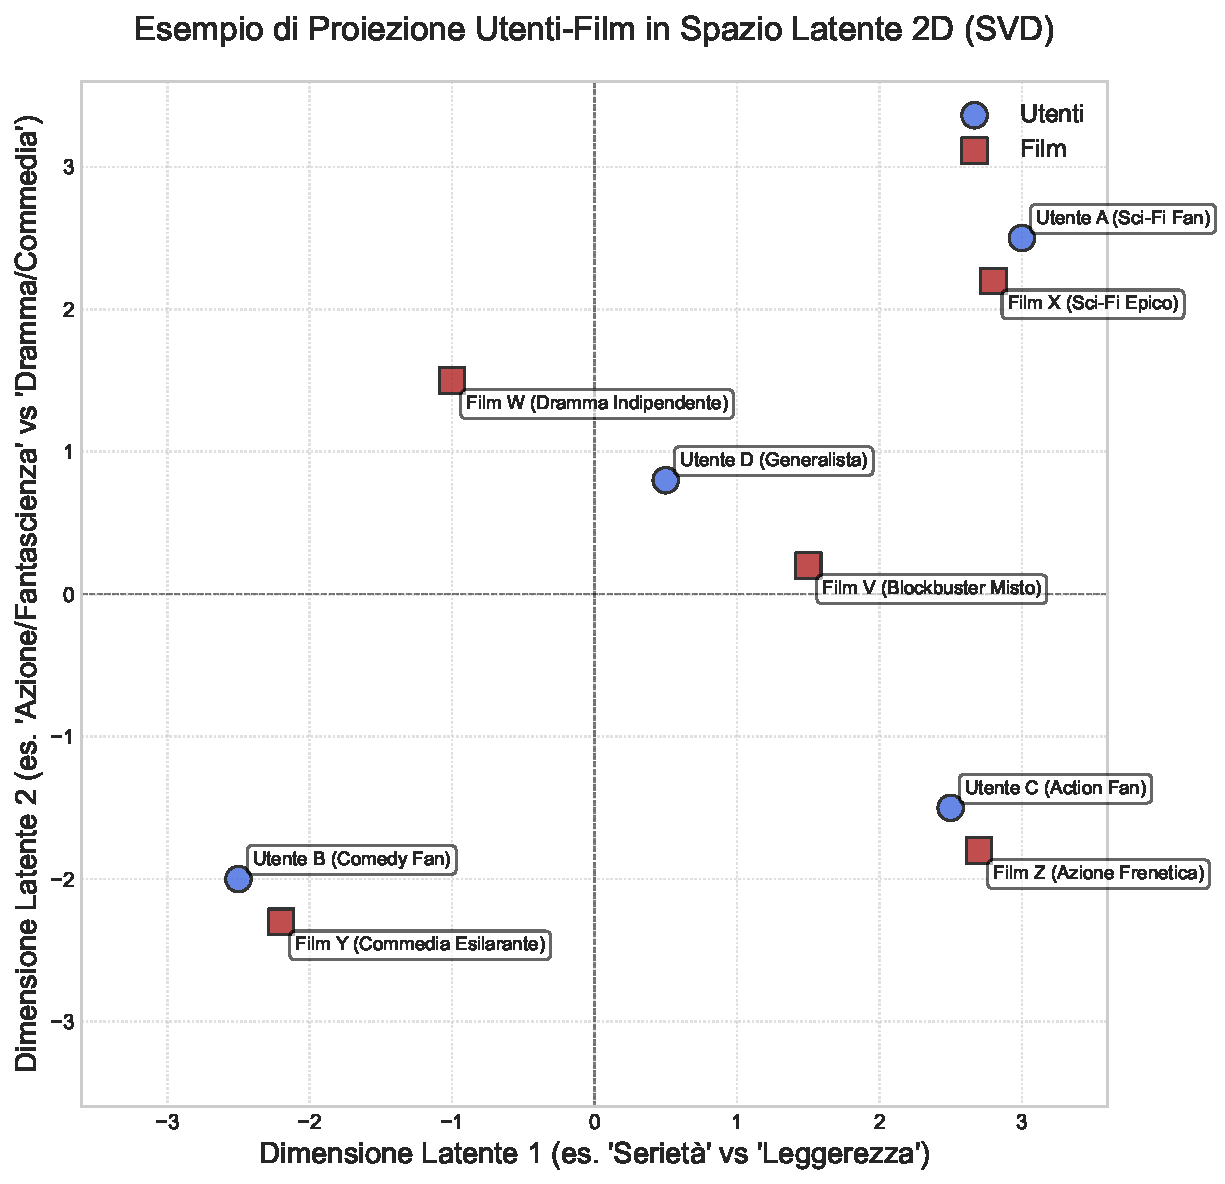
\includegraphics[width=0.8\textwidth]{images/svd_projection_example.pdf}
    \caption{Esempio di proiezione di utenti e film in uno spazio bidimensionale ($k=2$) tramite SVD. La vicinanza e l'allineamento angolare indicano preferenza.}
    \label{fig:svd_projection}
\end{figure}

La qualità della previsione dipende dalla scelta corretta di $k$. Valori tipici che danno buoni risultati sono tra 20 e 100 fattori. Un $k$ inadeguato può portare a un'accuratezza inferiore rispetto all'uso della matrice originale.

\subsubsection{Raccomandazioni con Regole Associative}
Le regole associative, comunemente utilizzate per la \textit{market basket analysis} (analisi del carrello della spesa), cercano di scoprire relazioni del tipo "se un utente acquista X, allora è probabile che acquisti anche Y".
Una regola associativa è un'implicazione statistica $X \rightarrow Y$, dove $X$ (antecedente) e $Y$ (conseguente) possono contenere uno o più prodotti.
L'accuratezza di una regola è misurata da:
\begin{itemize}
    \item \textbf{Supporto}: Frazione di tutte le transazioni che contengono sia $X$ che $Y$.
          $$ \text{supporto}(X \rightarrow Y) = \frac{\text{Num. transazioni contenenti } X \text{ e } Y}{\text{Num. totale transazioni}} $$
    \item \textbf{Confidenza}: Frazione delle transazioni contenenti $X$ che contengono anche $Y$.
          $$ \text{confidenza}(X \rightarrow Y) = \frac{\text{Num. transazioni contenenti } X \text{ e } Y}{\text{Num. transazioni contenenti } X} $$
\end{itemize}
Supporto e confidenza sono usati anche come soglie (cut-off) per selezionare le regole più significative.

Per formulare raccomandazioni, si possono trasformare i rating (es. 1-5 stelle) in valori binari (es. 1 se il voto è sopra la media dell'utente, 0 altrimenti). Si estraggono poi le regole associative dall'insieme delle transazioni (escludendo l'utente attivo). Per un utente attivo, si identificano i prodotti non ancora acquistati/valutati e si cercano le regole rilevanti (cioè, quelle il cui antecedente è stato acquistato dall'utente ma il conseguente no). Le raccomandazioni vengono ordinate in base alla confidenza delle regole e si propongono i conseguenti delle regole con confidenza più alta.

\subsubsection{Metodi Probabilistici}
L'idea di base dei metodi probabilistici è calcolare la probabilità che un utente $u$ esprima un certo rating $r$ per un prodotto $p$, dati i rating precedentemente espressi dall'utente e i rating di tutti gli altri utenti.
Utilizzando il teorema di Bayes, e assumendo (come nel Naive Bayes) che i rating $X_i$ dell'utente attivo sui prodotti $d$ siano condizionatamente indipendenti dato il rating $Y$ per il prodotto target $p$, si cerca il valore di $Y$ che massimizza la probabilità a posteriori $P(Y|X)$:
$$ P(Y|X) = \frac{P(X|Y)P(Y)}{P(X)} = \frac{\left(\prod_{i=1}^{d} P(X_i|Y)\right) P(Y)}{P(X)} $$
Dato che $P(X)$ è costante rispetto a $Y$, è sufficiente massimizzare $\left(\prod_{i=1}^{d} P(X_i|Y)\right) P(Y)$.
Un problema comune è che se per un dato $Y_i$ (un possibile rating per l'item target) nessun utente ha dato a un prodotto $X_j$ lo stesso voto dell'utente attivo, la probabilità condizionata $P(X_j|Y_i)$ diventa zero, azzerando l'intera probabilità $P(X|Y_i)$. Questo problema viene affrontato con tecniche di \textit{smoothing}.
Esistono tecniche più complesse che utilizzano clustering, Reti Bayesiane, PLSA (Probabilistic Latent Semantic Analysis), ecc..

\subsubsection{Slope One Predictor}
Proposto da Lemire e Maclachlan (2005), lo Slope One è un predittore semplice basato su un differenziale di popolarità tra gli item per gli utenti. L'idea è che la differenza media di rating tra due item, osservata tra gli utenti che li hanno valutati entrambi, possa essere usata per predire il rating di un utente per un item basandosi sul suo rating per l'altro item. Si cerca una funzione della forma $f(x) = x+b$ (da cui il nome "Slope One", pendenza unitaria).
Ad esempio, se l'utente Carl ha votato Item1 con 2 e l'utente Jack ha votato Item1 con 1 e Item5 con 3, la predizione per Carl su Item5 potrebbe essere $2 + (3-1) = 4$.
Generalizzando, si calcola la differenza media dei punteggi tra coppie di item (es. Item A e Item B) basandosi su tutti gli utenti che li hanno co-valutati. Per predire il voto di un utente Lucy per l'Item A, avendo i suoi voti per Item B e Item C, si usano queste differenze medie:
\begin{itemize}
    \item Voto per A basato su B: $r_{\text{Lucy,B}} + \text{diff\_media}(A,B)$
    \item Voto per A basato su C: $r_{\text{Lucy,C}} + \text{diff\_media}(A,C)$
\end{itemize}
Le diverse predizioni ottenute (una per ogni item che Lucy ha valutato e per cui esiste una differenza media calcolata) vengono poi combinate usando una media ponderata, dove il peso è tipicamente il numero di utenti che hanno co-valutato la coppia di item usata per calcolare la differenza.

\subsection{Considerazioni Finali sui Metodi Collaborative Filtering}
\begin{itemize}
    \item \textbf{Pro}: Sono facili da comprendere e implementare in forme base, e funzionano bene in diversi settori. Non richiedono una conoscenza approfondita delle caratteristiche degli item (come nei metodi content-based).
    \item \textbf{Contro}: Richiedono una "comunità" di utenti con un numero sufficiente di valutazioni per trovare pattern significativi. Soffrono di problemi di sparsità dei dati e del cold start. Non integrano facilmente altre fonti di conoscenza (es. attributi degli item o degli utenti).
    \item \textbf{Qual è il miglior metodo?}: È difficile stabilirlo in modo assoluto, le differenze tra i metodi sono spesso piccole (nell'ordine dell'1\%) e dipendono dal dataset e dal dominio specifico.
\end{itemize}

\begin{examplebox}{Sistema Reale: Google News (Cenni Teorici)}
    Google News aggrega notizie da migliaia di fonti e le visualizza agli utenti loggati in modo personalizzato. La raccomandazione si basa su un approccio collaborativo, considerando la storia dei click dell'utente attivo e della comunità.
    \textbf{Principali Sfide}:
    \begin{itemize}
        \item Vasto numero di articoli e utenti.
        \item Necessità di generare raccomandazioni in tempo reale (massimo un secondo).
        \item Flusso costante di nuovi item (notizie).
    \end{itemize}
    Queste sfide richiedono sforzi significativi in termini di algoritmi, ingegneria del software e parallelizzazione.
    Gli approcci memory-based puri non sono direttamente applicabili a questa scala, mentre con i model-based c'è il problema dell'aggiornamento continuo del modello. Google News utilizza una combinazione di tecniche model-based e memory-based:
    \begin{itemize}
        \item \textbf{Parte Model-based}: Tecniche di clustering come pLSI (Probabilistic Latent Semantic Indexing) e MinHash (per stimare la similarità di insiemi in modo efficiente).
        \item \textbf{Parte Memory-based}: Gestione dei nuovi utenti analizzando lo storico delle co-visite con altri utenti.
    \end{itemize}
    MapReduce (o tecnologie simili) viene utilizzata per parallelizzare la computazione e renderla scalabile.
\end{examplebox}
% Fine 07_Aula_Recommendation.pdf


\section{Introduzione alla Classificazione}

La classificazione è un compito fondamentale nel machine learning che consiste nell'assegnare una etichetta di classe (o categoria) a un'istanza (o osservazione) descritta da un insieme di caratteristiche (variabili o feature).

\paragraph{Cosa Significa Classificare?}L'obiettivo della classificazione è individuare una funzione (o un modello) che, data un'istanza di input, sia in grado di predire a quale classe essa appartenga. Questa funzione cerca di massimizzare la separazione tra le istanze appartenenti a classi diverse nello spazio delle feature.

\begin{examplebox}{Classificazione di Cellule Tumorali}
    Si consideri il problema di distinguere tra cellule cancerogene benigne e maligne.  Ogni cellula è descritta da diverse variabili misurabili, come l'area media delle concavità, il perimetro, la consistenza, il numero medio di concavità, la varianza della scala di grigi, ecc.
    Se rappresentiamo ogni cellula come un punto in un grafico dove gli assi corrispondono a due di queste variabili (es. area media sull'asse x e numero medio di concavità sull'asse y), le cellule maligne (es. rosse) e benigne (es. blu) potrebbero formare due insiemi distinti.  Il compito della classificazione è trovare una "linea" (o, più in generale, una superficie) che separi al meglio questi due insiemi di punti.
\end{examplebox}

\begin{figure}[H]
    \centering
    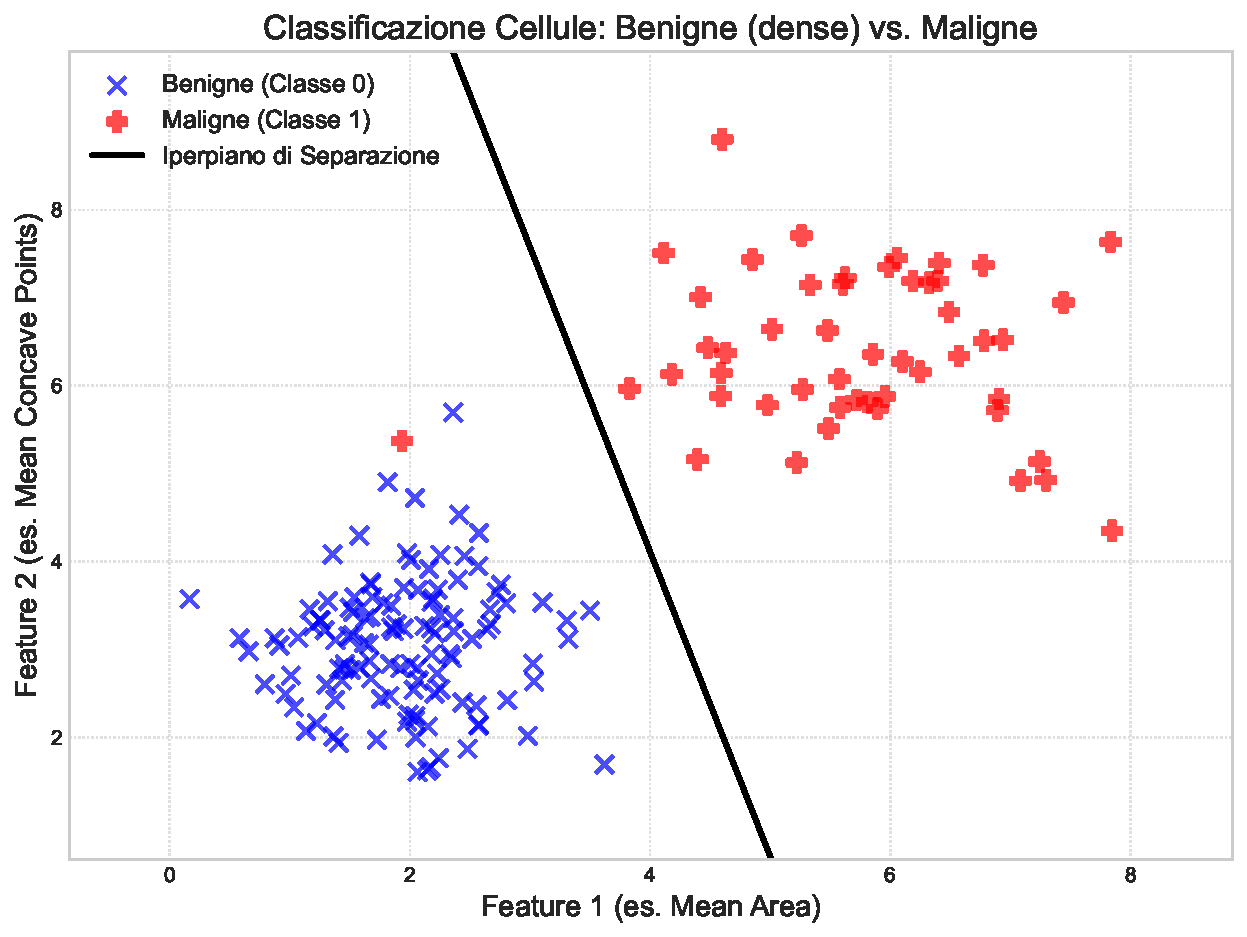
\includegraphics[width=0.7\textwidth]{images/cell_classification_scatter.pdf}
    \caption{Esempio di classificazione binaria: cellule maligne (rosse, '+') e benigne (blu, 'x') rappresentate in base a due feature (Mean Area, Mean Concave Points), con un possibile iperpiano di separazione lineare.}
    \label{fig:cell_classification_scatter}
\end{figure}

\subsection{Iperpiano di Separazione e Classificazione Lineare}
In molti problemi di classificazione binaria, si cerca un \textbf{iperpiano} che separi le istanze delle due classi. Se le feature di un'istanza $x_i$ sono rappresentate da un vettore, un iperpiano è definito dall'equazione:
$$ w^T x_i + b = 0 $$
dove $w$ è un vettore di pesi (ortogonale all'iperpiano) e $b$ è un termine di bias (o intercetta), proporzionale alla distanza dell'iperpiano dall'origine ($\frac{b}{||w||}$).

Una volta definito l'iperpiano, la classificazione di una nuova istanza $x$ avviene come segue:
\begin{itemize}
    \item Se $w^T x + b > 0$, l'istanza $x$ viene assegnata a una classe (es. classe +1, maligna).
    \item Se $w^T x + b < 0$, l'istanza $x$ viene assegnata all'altra classe (es. classe -1, benigna).
    \item Se $w^T x + b = 0$, l'istanza si trova esattamente sull'iperpiano (boundary).
\end{itemize}
La distanza $d$ di un punto $x$ dall'iperpiano $w^T x' + b = 0$ è data da:
$$ d = \frac{|w^T x + b|}{||w||} $$
Questa formula si deriva considerando che $w$ è ortogonale all'iperpiano.

\begin{figure}[H]
    \centering
    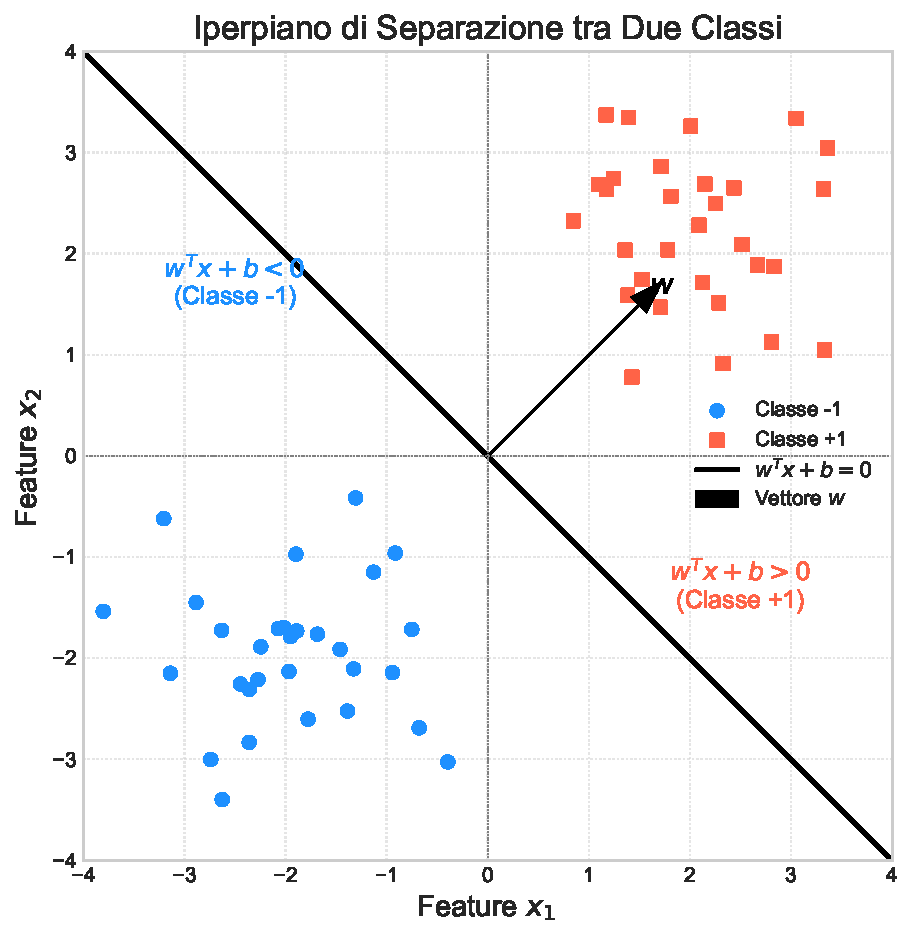
\includegraphics[width=0.6\textwidth]{images/hyperplane_separation.pdf}
    \caption{Iperpiano di separazione $w^T x + b = 0$ tra due classi.}
    \label{fig:hyperplane_separation}
\end{figure}

\subsubsection{Caratteristiche dei Classificatori Lineari}
Per un dato insieme di dati, possono esistere molteplici iperpiani (definiti da diverse coppie $w, b$) che separano le classi.
\begin{itemize}
    \item Alcuni metodi, come il Perceptron, la Regressione Logistica, o la regressione lineare usata con una soglia, individuano un iperpiano di separazione che potrebbe non essere ottimale secondo certi criteri (es. massimizzazione del margine).  Questi metodi sono generalmente influenzati da \textit{tutti} i punti del training set.
    \item Altri metodi, come le Support Vector Machines (SVM), cercano di individuare un iperpiano di separazione ottimale, ad esempio quello che massimizza la distanza dalle istanze più vicine di entrambe le classi. Le SVM sono influenzate principalmente dai "punti difficili", ovvero quelli vicini al confine di decisione (chiamati support vectors).
\end{itemize}

\subsubsection{Classificatore Perceptron}
Il Perceptron, introdotto da Rosenblatt nel 1957, è un algoritmo per l'apprendimento di un classificatore lineare binario.  L'obiettivo è trovare un vettore di pesi $w$ (che include implicitamente il bias $b$ se si aggiunge una feature $x_0=1$ a ogni istanza) tale che:
\begin{itemize}
    \item $w^T x > 0$ per le istanze di una classe (es. +1)
    \item $w^T x < 0$ per le istanze dell'altra classe (es. -1)
\end{itemize}
L'algoritmo del Perceptron è iterativo:
\begin{enumerate}
    \item Inizializza $w$ casualmente (o a zero).
    \item Ripeti:
          \begin{enumerate}
              \item classification\_error = false
              \item Per ogni istanza $x$ nel training set:
                    \begin{itemize}
                        \item Se $x$ è della classe -1 ma $w^T x \ge 0$ (errore): $w \leftarrow w - x$.  classification\_error = true.
                        \item Se $x$ è della classe +1 ma $w^T x \le 0$ (errore): $w \leftarrow w + x$.  classification\_error = true.
                    \end{itemize}
          \end{enumerate}
    \item Fino a quando classification\_error è false (cioè, nessuna istanza viene mal classificata nell'ultima iterazione).
\end{enumerate}
L'algoritmo del Perceptron converge solo se i dati sono linearmente separabili. È considerato un progenitore delle Reti Neurali.

\subsubsection{Come Trovare l'Iperpiano di Separazione? Funzione di Perdita (Loss Function)}
Per trovare i parametri $w$ e $b$ ottimali, si definisce una funzione di perdita (loss function) che misura l'errore di classificazione del modello sul training set. L'obiettivo è minimizzare questa funzione.
Se le etichette di classe sono $y_i \in \{-1, +1\}$, una condizione per la corretta classificazione dell'istanza $x_i$ con il modello $h_w(x_i) = w^T x_i + b$ è $y_i \cdot h_w(x_i) > 0$.  Se $y_i \cdot h_w(x_i) \le 0$, l'istanza è mal classificata.
Una possibile loss function (chiamata hinge loss implicita) è:
$$ L(w,b) = \sum_{i=1}^{m} \max(0, -y_i (w^T x_i + b)) $$
Questa funzione è zero se l'istanza è classificata correttamente e con un certo margine (se $-y_i (w^T x_i + b) < 0$), altrimenti restituisce un valore positivo proporzionale all'errore.
Tuttavia, questa funzione $\max(0,s)$ non è derivabile ovunque (nel punto $s=0$), il che rende difficile l'applicazione diretta della discesa del gradiente. Inoltre, ha un minimo fittizio per $w=0, b=0$.

\paragraph{Logistic Loss.}
Per superare i problemi della funzione $\max(0,s)$, si può sostituire con una sua approssimazione derivabile, come la funzione $softmax(0,s) = \log(1+e^s)$. La funzione di perdita da minimizzare diventa quindi la \textbf{Logistic Loss}:
$$ L(w,b) = \sum_{i=1}^{m} \log(1 + e^{-y_i (w^T x_i + b)}) $$
Questa funzione è convessa, continua e derivabile.  Si può aggiungere un termine di regolarizzazione L2 (o L1) per controllare la complessità del modello e prevenire l'overfitting:
$$ L_{\text{reg}}(w,b) = \sum_{i=1}^{m} \log(1 + e^{-y_i (w^T x_i + b)}) + \frac{\lambda}{2} ||w||_2^2 $$
I parametri $w, b$ (o $\tilde{w} = (b, w)$ se si include $b$ come $w_0$ e $x_0=1$) vengono poi appresi minimizzando questa funzione d'errore regolarizzata tramite la discesa del gradiente.

\subsection{Regressione Logistica}
Il classificatore lineare appreso minimizzando la logistic loss è utilizzato nella funzione sigmoide (o logistica), dando origine al modello di \textbf{Regressione Logistica}:
$$ \sigma(h_{\tilde{w}}(\tilde{x})) = \sigma(w^T x + b) = \frac{1}{1 + e^{-(w^T x + b)}} $$
Caratteristiche della Regressione Logistica:
\begin{itemize}
    \item Il codominio della funzione sigmoide è $[0, 1]$, quindi l'output $\sigma(h_{\tilde{w}}(\tilde{x}))$ può essere interpretato come la probabilità di appartenenza dell'istanza $\tilde{x}$ a una delle due classi (es. la classe +1).
    \item $P(Y=+1 | X=x^{(i)}) = \sigma(w^T x^{(i)} + b)$.
    \item $P(Y=-1 | X=x^{(i)}) = 1 - \sigma(w^T x^{(i)} + b)$.
    \item Se un'istanza $x$ si trova sull'iperpiano di separazione, $w^T x + b = 0$, allora $\sigma(0) = 0.5$.
    \item Se $w^T x + b > 0$, allora $\sigma(w^T x + b) > 0.5$, indicando una maggiore probabilità per la classe +1.
    \item Se $w^T x + b < 0$, allora $\sigma(w^T x + b) < 0.5$, indicando una maggiore probabilità per la classe -1.
\end{itemize}
La regressione logistica può essere estesa a casi non lineari introducendo feature polinomiali (o altre trasformazioni non lineari) delle variabili di input originali, $h_w^2(x_1, \dots, x_n) = \sum w_{ij} x_i x_j + \dots$. Il numero di termini generati e la potenziale non scalabilità seguono considerazioni simili a quelle viste per la regressione polinomiale, ma il problema può essere affrontato, ad esempio, con la kernel logistic regression (strettamente legata alle SVM).

\begin{figure}[H]
    \centering
    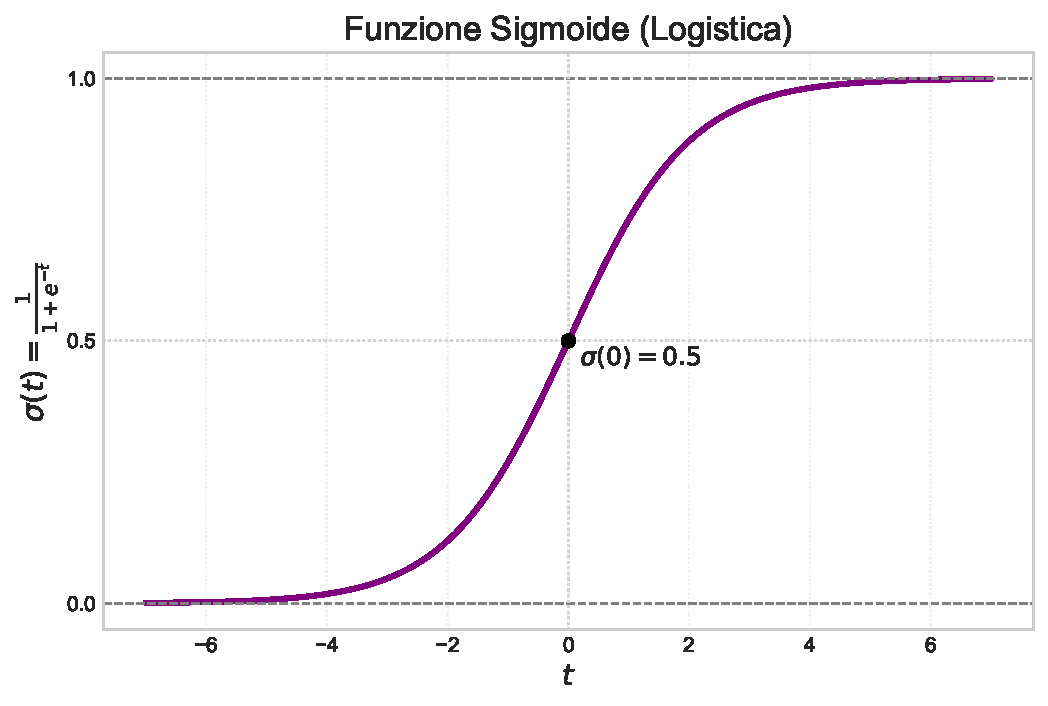
\includegraphics[width=0.6\textwidth]{images/sigmoid_function.pdf}
    \caption{Funzione sigmoide $\sigma(t)$.}
    \label{fig:sigmoid_function}
\end{figure}

\begin{notebox}{Regressione Logistica e Unità Neuronale}
    La funzione di regressione logistica $f(a) = \frac{1}{1+e^{-a}}$, dove $a = w^T x + b$ è l'output lineare (attivazione), è matematicamente equivalente a una singola unità neuronale (neurone) in una rete neurale artificiale con funzione di attivazione sigmoide. L'input $x$ con i pesi $w$ e il bias $b$ vengono sommati linearmente e poi passati attraverso la sigmoide per produrre l'output.
\end{notebox}

\subsection{Classificatori Non Lineari}
Molti problemi presentano dati che non sono linearmente separabili, ovvero non esiste un singolo iperpiano in grado di dividere correttamente le classi nello spazio delle feature originali. Per affrontare questi casi, si ricorre a classificatori non lineari. Esistono due approcci principali:
\begin{itemize}
    \item \textbf{Trasformazione dello Spazio dei Dati}: Alcuni metodi, come le Support Vector Machines (SVM) con kernel non lineari o le Reti Neurali, mappano i dati originali in uno spazio a dimensionalità superiore, dove si spera che le classi diventino linearmente separabili. Successivamente, un classificatore lineare viene applicato in questo nuovo spazio trasformato. Più variabili (dimensioni) hanno i dati trasformati, maggiori sono le chance di trovare una separazione lineare.
    \item \textbf{Soluzioni Intrinsecamente Non Lineari}: Altri metodi, come k-Nearest Neighbors (KNN), Alberi Decisionali (Decision Trees), Random Forest, Gradient Boosting (e varianti come XGBoost, LightGBM, CatBoost), definiscono confini di decisione intrinsecamente non lineari nello spazio originale delle feature.
\end{itemize}

\begin{figure}[H]
    \centering
    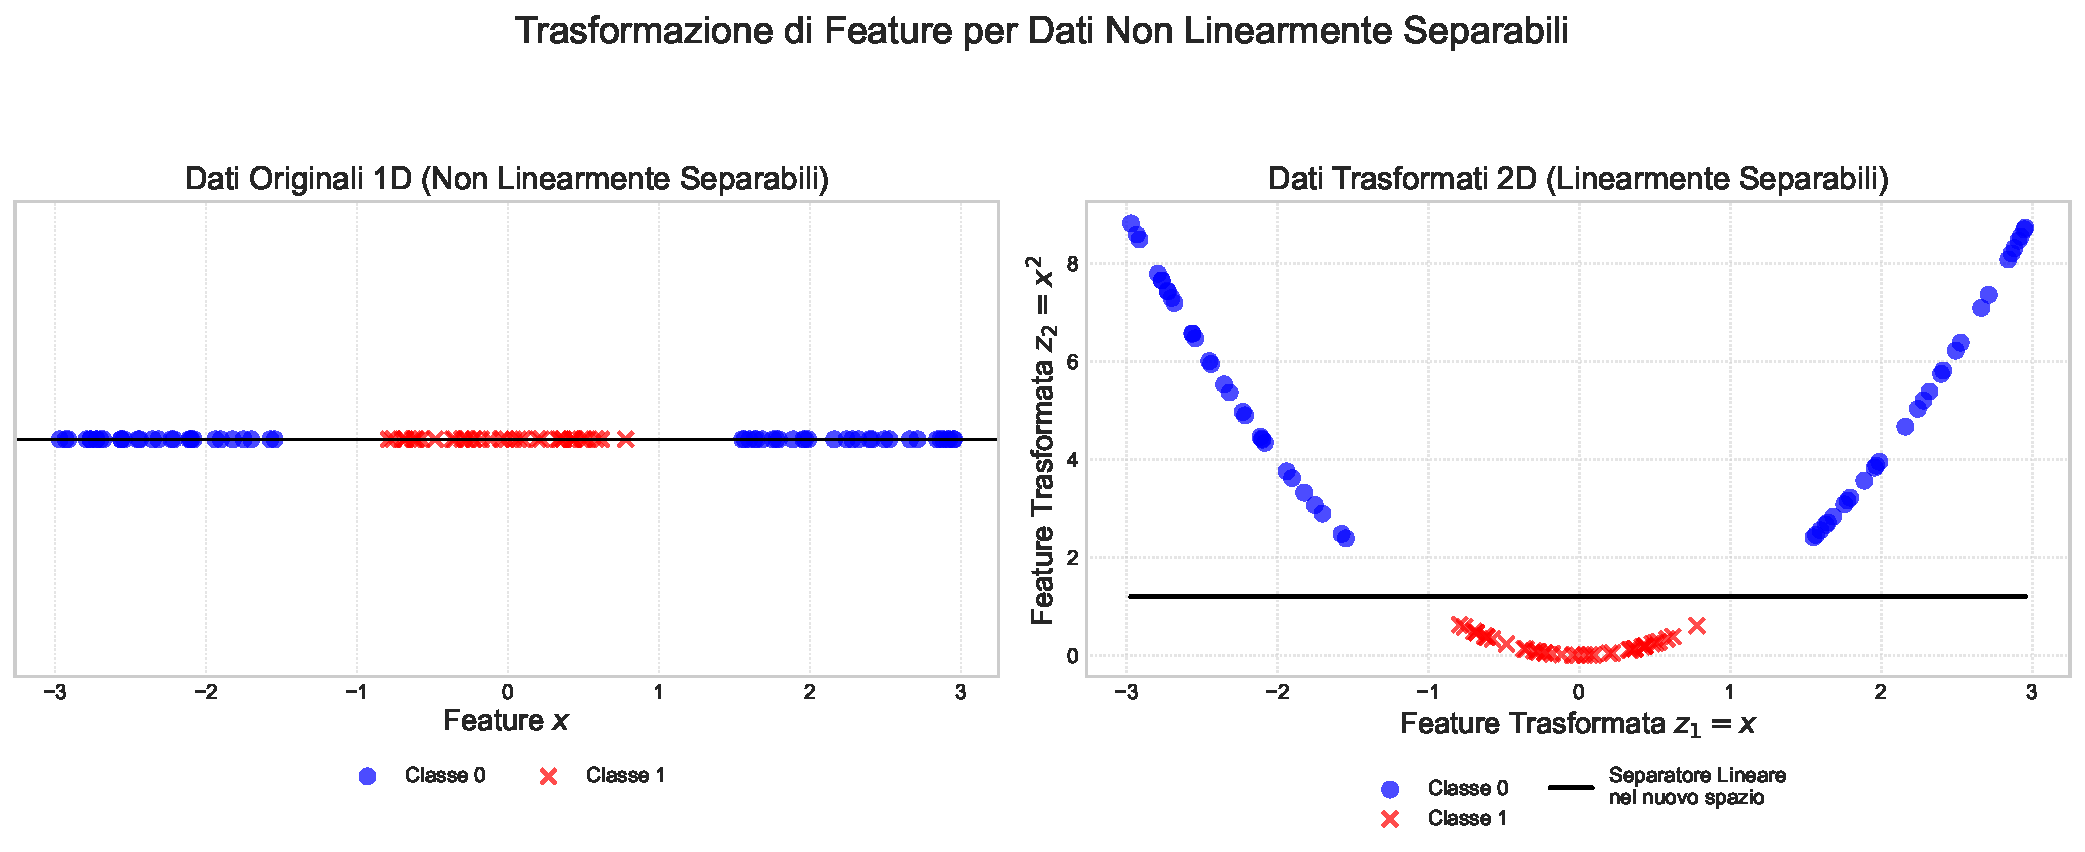
\includegraphics[width=1\textwidth]{images/nonlinear_data_transformation.pdf}
    \caption{Esempio di dati non linearmente separabili (sinistra) e come una trasformazione dello spazio (es. $x \rightarrow (x, x^2)$) può renderli linearmente separabili (destra).}
    \label{fig:nonlinear_data_transformation}
\end{figure}

\subsection{Classificazione Multi-Classe con Iperpiani}
Molti classificatori lineari, come il Perceptron, la Regressione Logistica e le SVM (nella loro formulazione base), sono intrinsecamente binari, cioè progettati per distinguere tra due sole classi. Per estenderli a problemi con $C > 2$ classi, si utilizzano comunemente due strategie principali:

\begin{enumerate}
    \item \textbf{One-Versus-All (OvA) o One-Versus-Rest (OvR)}:
          \begin{itemize}
              \item Si addestrano $C$ classificatori binari distinti.
              \item Ciascun classificatore $c$ impara a separare le istanze della classe $c$ da tutte le istanze delle altre $C-1$ classi (considerate come un'unica classe "resto"). L'iperpiano per il classificatore $c$ è $b_c + w_c^T x = 0$.
              \item Questo metodo è parallelizzabile, poiché i $C$ classificatori possono essere addestrati indipendentemente.
              \item \textbf{Regola di Fusione}: Per classificare una nuova istanza $x$, si calcola l'output di ciascuno dei $C$ classificatori. L'istanza viene assegnata alla classe $j$ per la quale l'output del classificatore $j$ (spesso interpretato come una "fiducia" o distanza dall'iperpiano) è massimo:
                    $$ y_{\text{pred}} = \arg\max_{j=1,\dots,C} (b_j + w_j^T x) $$
          \end{itemize}

    \item \textbf{Multinomial (o Softmax Regression per generalizzazione della Logistica)}:
          \begin{itemize}
              \item Si individuano congiuntamente $C$ iperpiani (o funzioni lineari) cercando di ottimizzare direttamente una regola di fusione che consideri tutte le classi contemporaneamente.
              \item Nel caso della generalizzazione multinomiale della regressione logistica, si utilizza la funzione \textbf{softmax} per convertire gli score lineari $s_j = b_j + w_j^T x$ (per $j=1,\dots,C$) in probabilità di appartenenza a ciascuna classe:
                    $$ P(Y=j | x) = \frac{e^{s_j}}{\sum_{k=1}^{C} e^{s_k}} $$
              \item La funzione di perdita da minimizzare è tipicamente la \textit{cross-entropy loss} (o negative log-likelihood). Ad esempio, se $y^{(i)}$ è la vera classe (one-hot encoded) per l'istanza $x^{(i)}$ e $p_j^{(i)}$ è la probabilità predetta per la classe $j$:
                    $$ L = - \sum_{i=1}^{m} \sum_{j=1}^{C} y_j^{(i)} \log(p_j^{(i)}) $$
                    Alternativamente, si può minimizzare una funzione basata sulla differenza tra lo score massimo e lo score della classe corretta, utilizzando una versione "soft" della funzione max.
          \end{itemize}
\end{enumerate}

\subsection{Classificazione con Classi Sbilanciate}
In molti problemi reali, la distribuzione delle istanze tra le classi è fortemente sbilanciata. Ad esempio:
\begin{itemize}
    \item Nelle transazioni con carte di credito, le transazioni lecite sono molto più numerose di quelle illecite (frodi).
    \item Nella diagnosi di malattie rare, i casi negativi sono molto più frequenti dei positivi.
    \item Nell'analisi della \textit{churn} (abbandono dei clienti), i clienti fedeli sono generalmente più numerosi di quelli che abbandonano il servizio.
\end{itemize}
Quando le classi sono sbilanciate, molti algoritmi di classificazione tendono a favorire la classe maggioritaria, portando a un numero elevato di errori di classificazione sulla classe minoritaria, che è spesso quella di maggiore interesse. Questo può portare a risultati inaccettabili.
\textbf{Rimedi} per mitigare il problema:
\begin{itemize}
    \item \textbf{Pesatura degli Errori (Cost-sensitive learning)}: Aumentare il peso assegnato agli errori di classificazione sulla classe con meno istanze. Molti modelli permettono di specificare un parametro `class\_weight` (es. `{classe\_minoritaria: peso\_maggiore, classe\_maggioritaria: 1.0}`). Il peso ottimale può essere trovato tramite tecniche come la grid search.
    \item \textbf{Ricampionamento (Resampling)}:
          \begin{itemize}
              \item \textbf{Undersampling}: Ridurre il numero di istanze della classe maggioritaria, selezionandone casualmente un sottoinsieme.
              \item \textbf{Oversampling}: Aumentare il numero di istanze della classe minoritaria, ad esempio duplicando istanze esistenti o generando nuove istanze sintetiche (es. con la tecnica SMOTE - Synthetic Minority Over-sampling TEchnique).
          \end{itemize}
\end{itemize}

\begin{figure}[H]
    \centering
    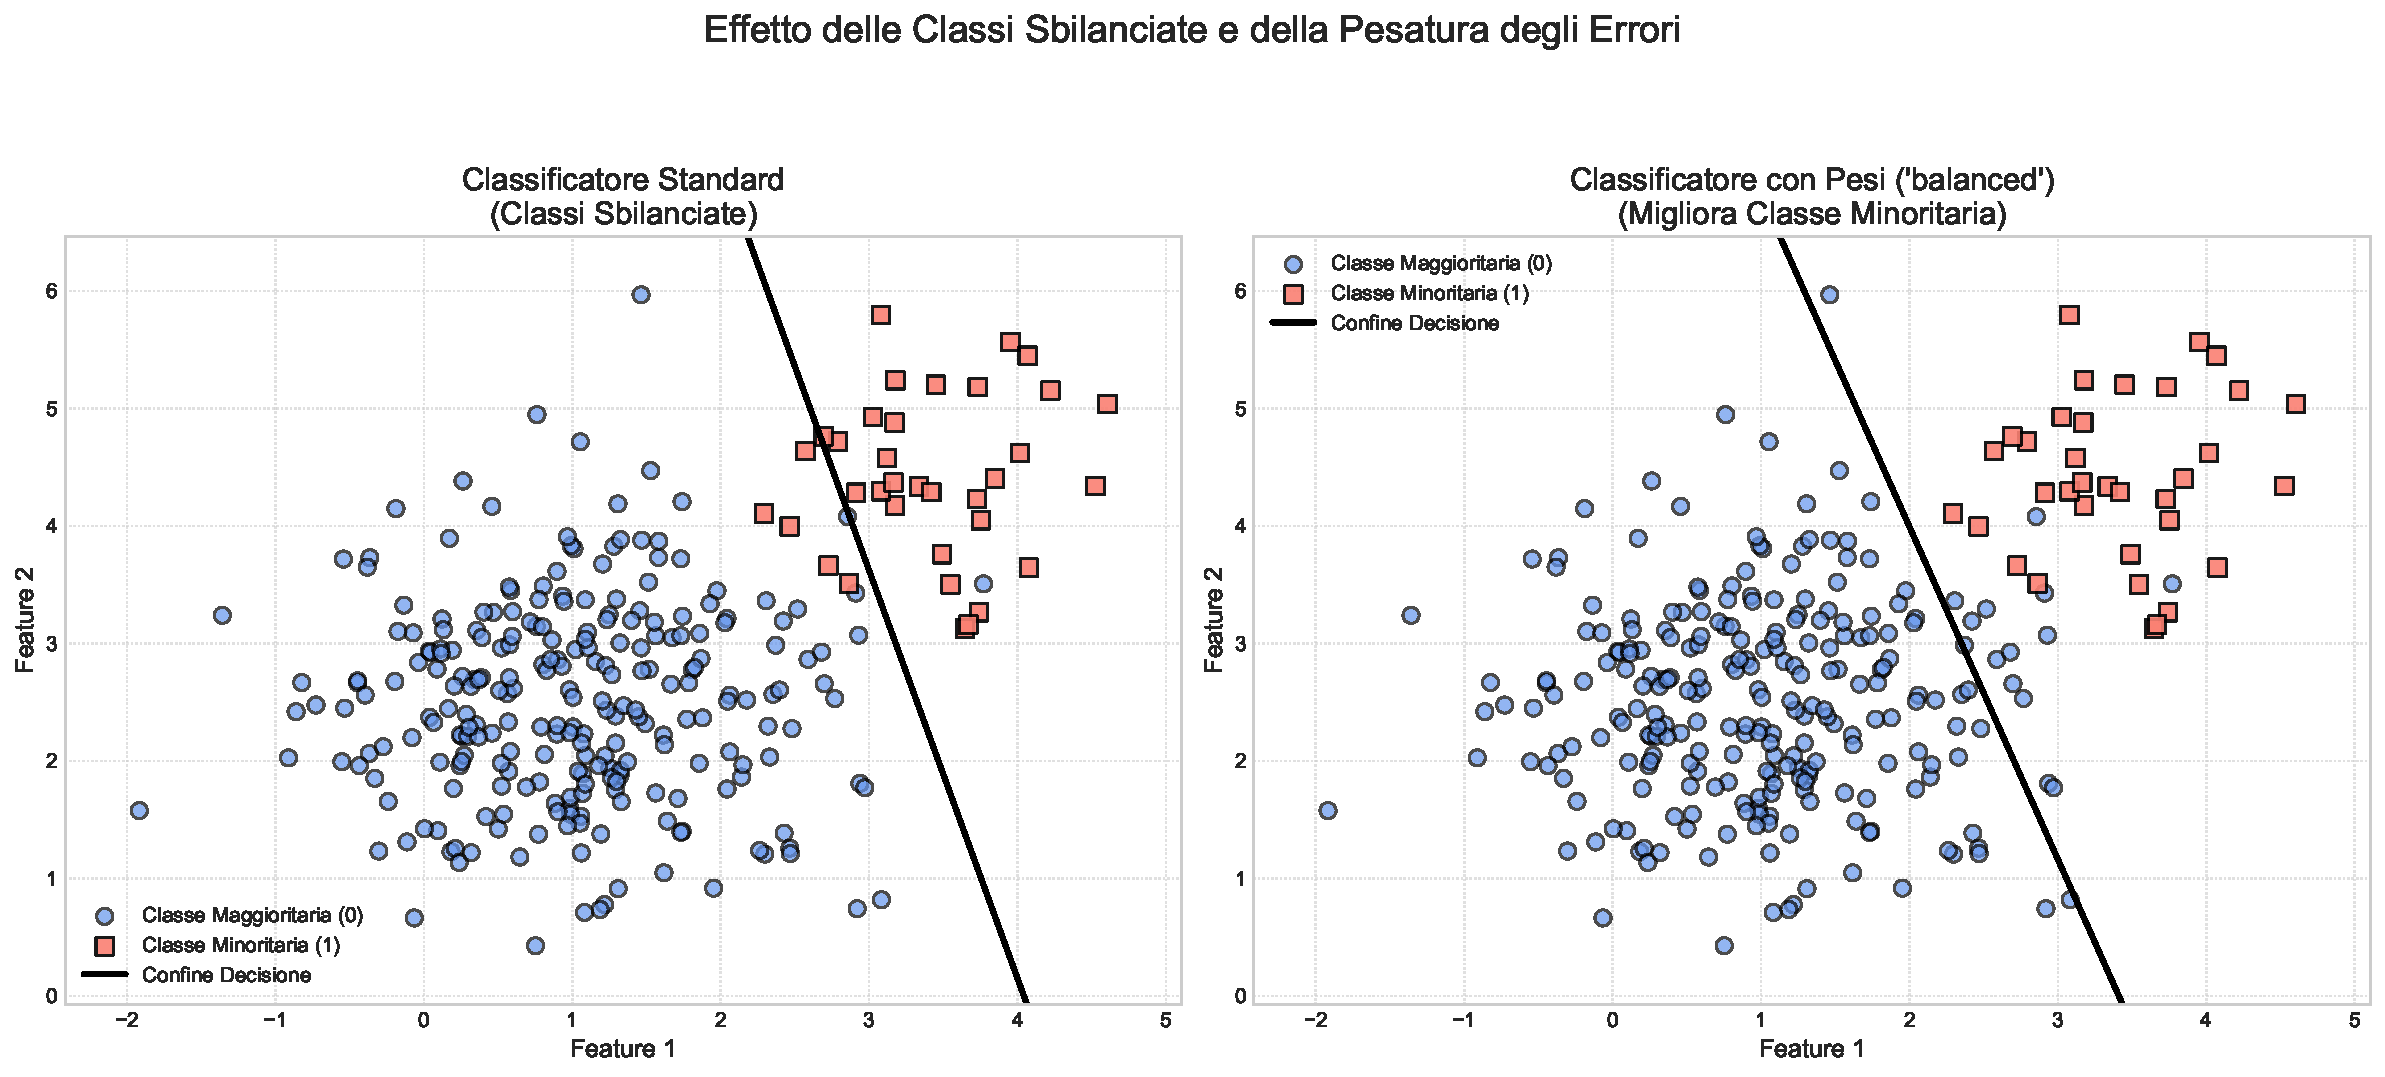
\includegraphics[width=1\textwidth]{images/imbalanced_classes.pdf}
    \caption{Effetto delle classi sbilanciate su un classificatore lineare e come la pesatura degli errori può migliorare la separazione per la classe minoritaria.}
    \label{fig:imbalanced_classes}
\end{figure}

\customhr
\subsection{Support Vector Machines (SVM) \textit{(Approfondimento)}}
I classificatori come il Perceptron e la Regressione Logistica individuano un iperpiano di separazione, ma tra i molti possibili iperpiani che potrebbero separare i dati (specialmente se linearmente separabili), non hanno un criterio intrinseco per stabilire quale sia il "migliore" in termini di generalizzazione, al di là della minimizzazione dell'errore sul training set (la regolarizzazione aiuta a vincolare la soluzione).

\subsubsection{L'Idea del Margine Massimo}
L'idea fondamentale dietro le Support Vector Machines (SVM) è quella di trovare l'iperpiano di separazione che massimizzi il \textbf{margine} tra le istanze delle due classi. Il margine è definito come la distanza tra l'iperpiano di separazione e le istanze più vicine di ciascuna classe. Queste istanze più vicine, che "supportano" o definiscono l'iperpiano ottimale, sono chiamate \textbf{support vectors}.
Un iperpiano con un margine maggiore tende ad avere una migliore capacità di generalizzazione e a essere meno sensibile a piccole variazioni nei dati di training (minore overfitting). Se si rimuovessero tutte le istanze che non sono support vectors, l'iperpiano calcolato rimarrebbe il medesimo.
La ricerca di questo iperpiano si traduce in un problema di ottimizzazione quadratica.

\begin{figure}[H]
    \centering
    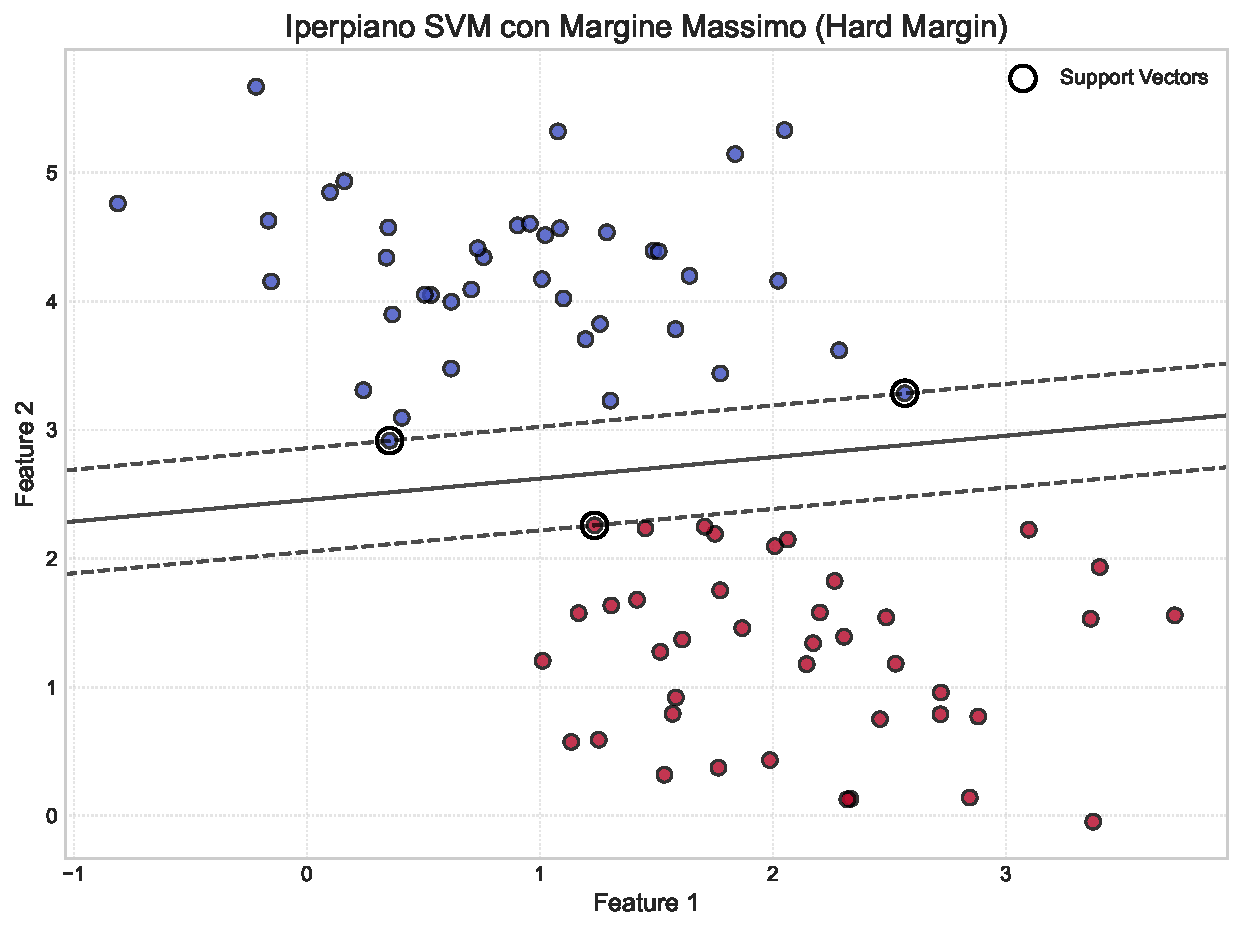
\includegraphics[width=0.7\textwidth]{images/max_margin_hyperplane.pdf}
    \caption{Iperpiano di separazione con margine massimo. I punti sui bordi del margine sono i support vectors.}
    \label{fig:max_margin_hyperplane}
\end{figure}

\subsubsection{Definizione del Problema SVM (Caso Lineare Separaibile)}
Sia $D = \{(x_i, y_i), \dots, (x_m, y_m)\}$ l'insieme delle $m$ istanze di training, dove $x_i \in \mathbb{R}^n$ è il vettore delle feature dell'istanza $i$-esima e $y_i \in \{-1, +1\}$ è la sua etichetta di classe.
Si cerca un iperpiano $w^T x + b = 0$ che non solo separi le classi, ma che lo faccia con il margine massimo.
Si definiscono due iperpiani paralleli a quello di separazione, passanti per i support vector delle due classi:
\begin{itemize}
    \item $w^T x + b = 1$ per i support vector della classe +1.
    \item $w^T x + b = -1$ per i support vector della classe -1.
\end{itemize}
Per tutte le altre istanze, si deve avere $w^T x_i + b \ge 1$ se $y_i = +1$, e $w^T x_i + b \le -1$ se $y_i = -1$. Queste due condizioni possono essere scritte in forma compatta come:
$$ y_i (w^T x_i + b) \ge 1 \quad \forall i=1, \dots, m $$
Il margine $\rho$ tra i due iperpiani $w^T x + b = 1$ e $w^T x + b = -1$ è la distanza tra di essi, che si può dimostrare essere $\rho = \frac{2}{||w||}$.
Massimizzare il margine $\rho = \frac{2}{||w||}$ è equivalente a minimizzare $||w||$, o, per convenienza matematica (per rimuovere la radice quadrata e avere una funzione quadratica), minimizzare $\frac{1}{2} ||w||^2 = \frac{1}{2} w^T w$.

Il problema di ottimizzazione per le SVM lineari con margine "hard" (hard-margin SVM, che assume che i dati siano linearmente separabili) è quindi:
$$ \min_{w,b} \frac{1}{2} w^T w $$
soggetto ai vincoli:
$$ y_i (w^T x_i + b) \ge 1 \quad \text{per } i=1, \dots, m $$
Questo è un problema di programmazione quadratica convessa, che ha una soluzione unica. La soluzione viene tipicamente trovata utilizzando i moltiplicatori di Lagrange.

\paragraph{Funzione di Classificazione SVM.}
Una volta trovati $w$ e $b$ ottimali, la funzione di classificazione per una nuova istanza $z$ è:
$$ f(z) = \text{sign}(w^T z + b) $$
È interessante notare che il vettore $w$ può essere espresso come una combinazione lineare dei soli support vector $x_k$: $w = \sum_{k \in SV} \alpha_k y_k x_k$, dove $\alpha_k$ sono i moltiplicatori di Lagrange (non nulli solo per i support vector). Sostituendo, la funzione di classificazione diventa:
$$ f(z) = \text{sign} \left( \sum_{k \in SV} \alpha_k y_k (x_k^T z) + b \right) $$
La classificazione dipende quindi solo dal prodotto scalare tra la nuova istanza $z$ e i support vector. Il bias $b$ può essere calcolato usando un qualsiasi support vector $x_k$: $b = y_k - w^T x_k$.

\subsubsection{SVM: Classificazione Multi-Classe}
Le SVM, nella loro formulazione originale, sono classificatori binari. Per applicarle a problemi di classificazione con $K > 2$ classi, si possono adottare diverse strategie:
\begin{itemize}
    \item \textbf{One-Versus-All (OvA) o One-Versus-Rest (OvR)}: Si addestrano $K$ classificatori SVM binari. Ciascun classificatore $k$ impara a separare le istanze della classe $k$ da tutte le istanze delle altre $K-1$ classi. Una nuova istanza viene classificata assegnandole la classe del classificatore che produce l'output (o "fiducia") più alto. Questa strategia è adatta anche a problemi multi-label (dove un'istanza può appartenere a più classi contemporaneamente).
    \item \textbf{One-Versus-One (OvO)}: Si addestra un classificatore SVM binario per ogni possibile coppia di classi. Questo porta a $\frac{K(K-1)}{2}$ classificatori. Una nuova istanza viene classificata sottoponendola a tutti i classificatori e utilizzando una strategia di voto maggioritario (o un altro schema di aggregazione) per determinare la classe finale.
    \item \textbf{Riformulazione Diretta Multi-Classe}: Esistono anche formulazioni del problema di ottimizzazione SVM che estendono direttamente l'approccio a $K$ classi, cercando di trovare simultaneamente tutti i confini di decisione.
\end{itemize}

\subsubsection{Margine Soft e Istanze Mal Classificate}
La formulazione SVM con margine "hard" (hard-margin) assume che i dati siano linearmente separabili e non ammette errori di classificazione sul training set. Tuttavia, molti dataset reali non sono perfettamente separabili linearmente, oppure contengono rumore o outlier. In questi casi, un margine hard potrebbe non esistere o portare a un modello con overfitting.
Per gestire queste situazioni, si introduce il concetto di \textbf{margine soft} (soft-margin SVM). L'idea è di permettere che alcune istanze del training set vengano mal classificate o si trovino all'interno della zona di margine, introducendo una penalità per tali violazioni. Si cerca un trade-off tra la massimizzazione del margine e la minimizzazione del numero di errori di classificazione.

\paragraph{Variabili Slack ($\xi_i$).}
Per permettere violazioni del margine, si introducono le \textbf{variabili slack} (o di comodo) $\xi_i \ge 0$, una per ogni istanza di training $x_i$. Queste variabili misurano il grado di violazione del margine per l'istanza $i$-esima:
\begin{itemize}
    \item Se $\xi_i = 0$, l'istanza $x_i$ è classificata correttamente e si trova dal lato corretto del margine (o esattamente sul bordo del margine per la sua classe).
    \item Se $0 < \xi_i \le 1$, l'istanza $x_i$ è classificata correttamente, ma si trova all'interno della zona di margine (tra l'iperpiano di separazione e il bordo del margine per la sua classe). Diventa un support vector.
    \item Se $\xi_i > 1$, l'istanza $x_i$ è mal classificata (si trova dal lato sbagliato dell'iperpiano di separazione). Diventa un support vector.
\end{itemize}
Le variabili slack "spostano" virtualmente le istanze misclassified o quelle dentro il margine per permettere la definizione di un iperpiano. Minimizzare solo il margine con queste trasformazioni potrebbe portare a soluzioni degeneri (margine troppo ampio); perciò, si minimizza anche la somma delle variabili slack.

\paragraph{Ottimizzazione con Margine Soft.}
Il problema di ottimizzazione per le SVM con margine soft diventa:
$$ \min_{w,b,\xi} \frac{1}{2} w^T w + C \sum_{i=1}^{m} \xi_i $$
soggetto ai vincoli:
$$ y_i (w^T x_i + b) \ge 1 - \xi_i \quad \text{per } i=1, \dots, m $$
$$ \xi_i \ge 0 \quad \text{per } i=1, \dots, m $$
L'iperparametro $C > 0$ controlla il trade-off tra la massimizzazione del margine (associata a $\frac{1}{2} w^T w$ piccolo) e la minimizzazione dell'errore di classificazione sul training set (associata a $\sum \xi_i$ piccolo).
\begin{itemize}
    \item Un valore di $C$ \textbf{grande} assegna un peso elevato agli errori di training $\xi_i$. L'ottimizzatore cercherà di minimizzare il numero di errori, portando a un margine più stretto e potenzialmente a overfitting.
    \item Un valore di $C$ \textbf{piccolo} aumenta la tolleranza agli errori di training, permettendo un margine più ampio e potenzialmente una migliore generalizzazione.
\end{itemize}
La funzione di classificazione finale per una nuova istanza $z$ ha la stessa forma del caso hard-margin:
$$ f(z) = \text{sign} \left( \sum_{k \in SV} \alpha_k y_k (x_k^T z) + b \right) $$
Tuttavia, i valori dei moltiplicatori di Lagrange $\alpha_k$ e l'insieme dei support vector $SV$ saranno diversi a causa della diversa formulazione del problema di ottimizzazione. I coefficienti $\alpha_k$ sono vincolati da $0 \le \alpha_k \le C$.

\begin{figure}[H]
    \centering
    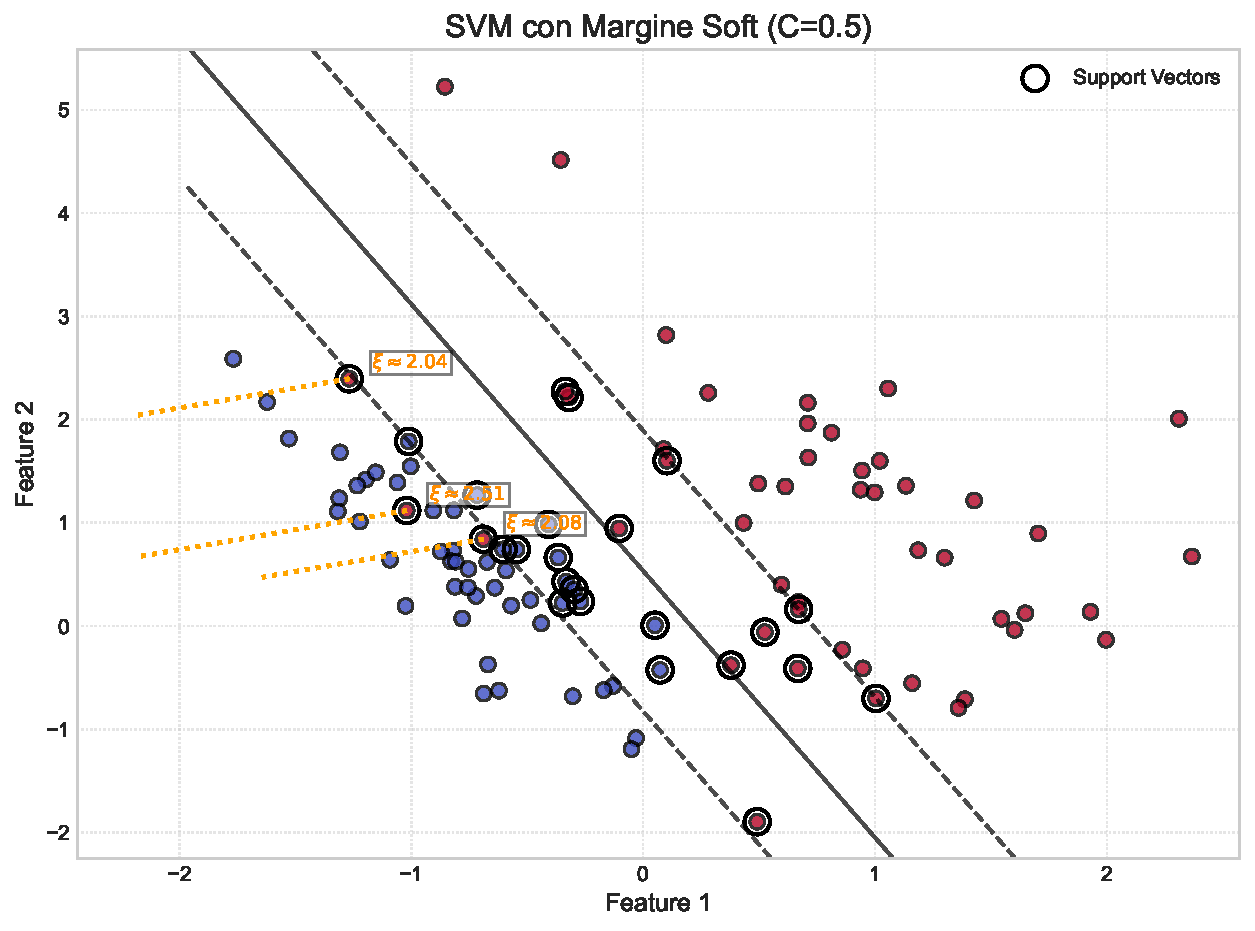
\includegraphics[width=0.7\textwidth]{images/soft_margin_svm.pdf}
    \caption{SVM con margine soft: le variabili slack $\xi_i$ permettono la gestione di istanze misclassified o all'interno del margine. L'iperparametro C bilancia la larghezza del margine con il numero di errori.}
    \label{fig:soft_margin_svm}
\end{figure}

\subsubsection{SVM Non Lineari e Funzioni Kernel}
Per dati che non sono linearmente separabili neanche con un margine soft, le SVM possono essere estese per trovare confini di decisione non lineari. L'idea principale è mappare i dati originali $x$ dallo spazio delle feature originali $\mathbb{R}^n$ in uno spazio a dimensionalità superiore $\mathbb{R}^N$ (con $N > n$, a volte $N$ è infinito) utilizzando una funzione di mapping non lineare $\phi: x \mapsto \phi(x)$. In questo spazio trasformato ad alta dimensionalità, si spera che i dati diventino linearmente separabili, permettendo l'applicazione di una SVM lineare.

\paragraph{Ottimizzazione nello Spazio Trasformato.}
Il problema di ottimizzazione SVM (con margine soft) viene formulato nello spazio trasformato:
$$ \min_{w_{\phi},b,\xi} \frac{1}{2} w_{\phi}^T w_{\phi} + C \sum_{i=1}^{m} \xi_i $$
soggetto ai vincoli:
$$ y_i (w_{\phi}^T \phi(x_i) + b) \ge 1 - \xi_i $$
$$ \xi_i \ge 0 $$
La funzione di classificazione per una nuova istanza $z$ diventa:
$$ f(z) = \text{sign} \left( \sum_{k \in SV} \alpha_k y_k (\phi(x_k)^T \phi(z)) + b \right) $$
Nota che la formulazione dipende solo dai prodotti scalari $\phi(x_k)^T \phi(z)$ dei vettori trasformati.

\paragraph{La Maledizione della Dimensionalità e il Kernel Trick.}
Mappare esplicitamente i dati in uno spazio a dimensionalità molto elevata può essere computazionalmente proibitivo ("maledizione della dimensionalità"). Ad esempio, una trasformazione polinomiale di grado $g$ su $n$ variabili originali può generare un numero di nuove feature dell'ordine di $O(n^g)$.
Il \textbf{Kernel Trick} permette di superare questo problema. Se il prodotto scalare nello spazio trasformato $\phi(x)^T \phi(z)$ può essere calcolato efficientemente usando una \textbf{funzione kernel} $K(x,z)$ applicata direttamente ai dati originali $x, z$, allora non è necessario calcolare esplicitamente la trasformazione $\phi$.
$$ K(x,z) = \phi(x)^T \phi(z) $$
Sostituendo $K(x,z)$ nella funzione di classificazione:
$$ f(z) = \text{sign} \left( \sum_{k \in SV} \alpha_k y_k K(x_k, z) + b \right) $$
Anche il problema di ottimizzazione può essere riformulato per dipendere solo dalla matrice kernel $K_{ij} = K(x_i, x_j)$. Il costo computazionale del training e della classificazione dipende quindi dal calcolo della funzione kernel $K$ sui dati originali, che è spesso molto più efficiente rispetto all'esplicita trasformazione $\phi$.

\paragraph{Teorema di Mercer.}
Una funzione $K(x,z)$ può essere usata come kernel se e solo se soddisfa certe condizioni matematiche (Teorema di Mercer), principalmente deve essere una funzione semi-definita positiva. Questo garantisce che $K(x,z)$ corrisponda a un prodotto scalare in qualche spazio delle feature (eventualmente a dimensione infinita).

\paragraph{Esempi Comuni di Funzioni Kernel.}
\begin{itemize}
    \item \textbf{Kernel Lineare}: $K(x,z) = x^T z$. Corrisponde alla SVM lineare standard.
    \item \textbf{Kernel Polinomiale}: $K(x,z) = (x^T z + c)^g$. Gli iperparametri sono il grado $g$ e la costante $c$. Permette di creare confini di decisione polinomiali.
    \item \textbf{Kernel Gaussiano (Radial Basis Function - RBF)}: $K(x,z) = \exp(-\gamma ||x-z||^2)$, dove $\gamma = \frac{1}{2\sigma^2}$ è un iperparametro che controlla l'ampiezza della gaussiana. Questo kernel è molto potente e può modellare confini di decisione complessi. Corrisponde a una mappatura in uno spazio a infinite dimensioni.
    \item \textbf{Kernel Sigmoidale (o Tangente Iperbolica)}: $K(x,z) = \tanh(k x^T z - \delta)$.
\end{itemize}

\begin{figure}[H]
    \centering
    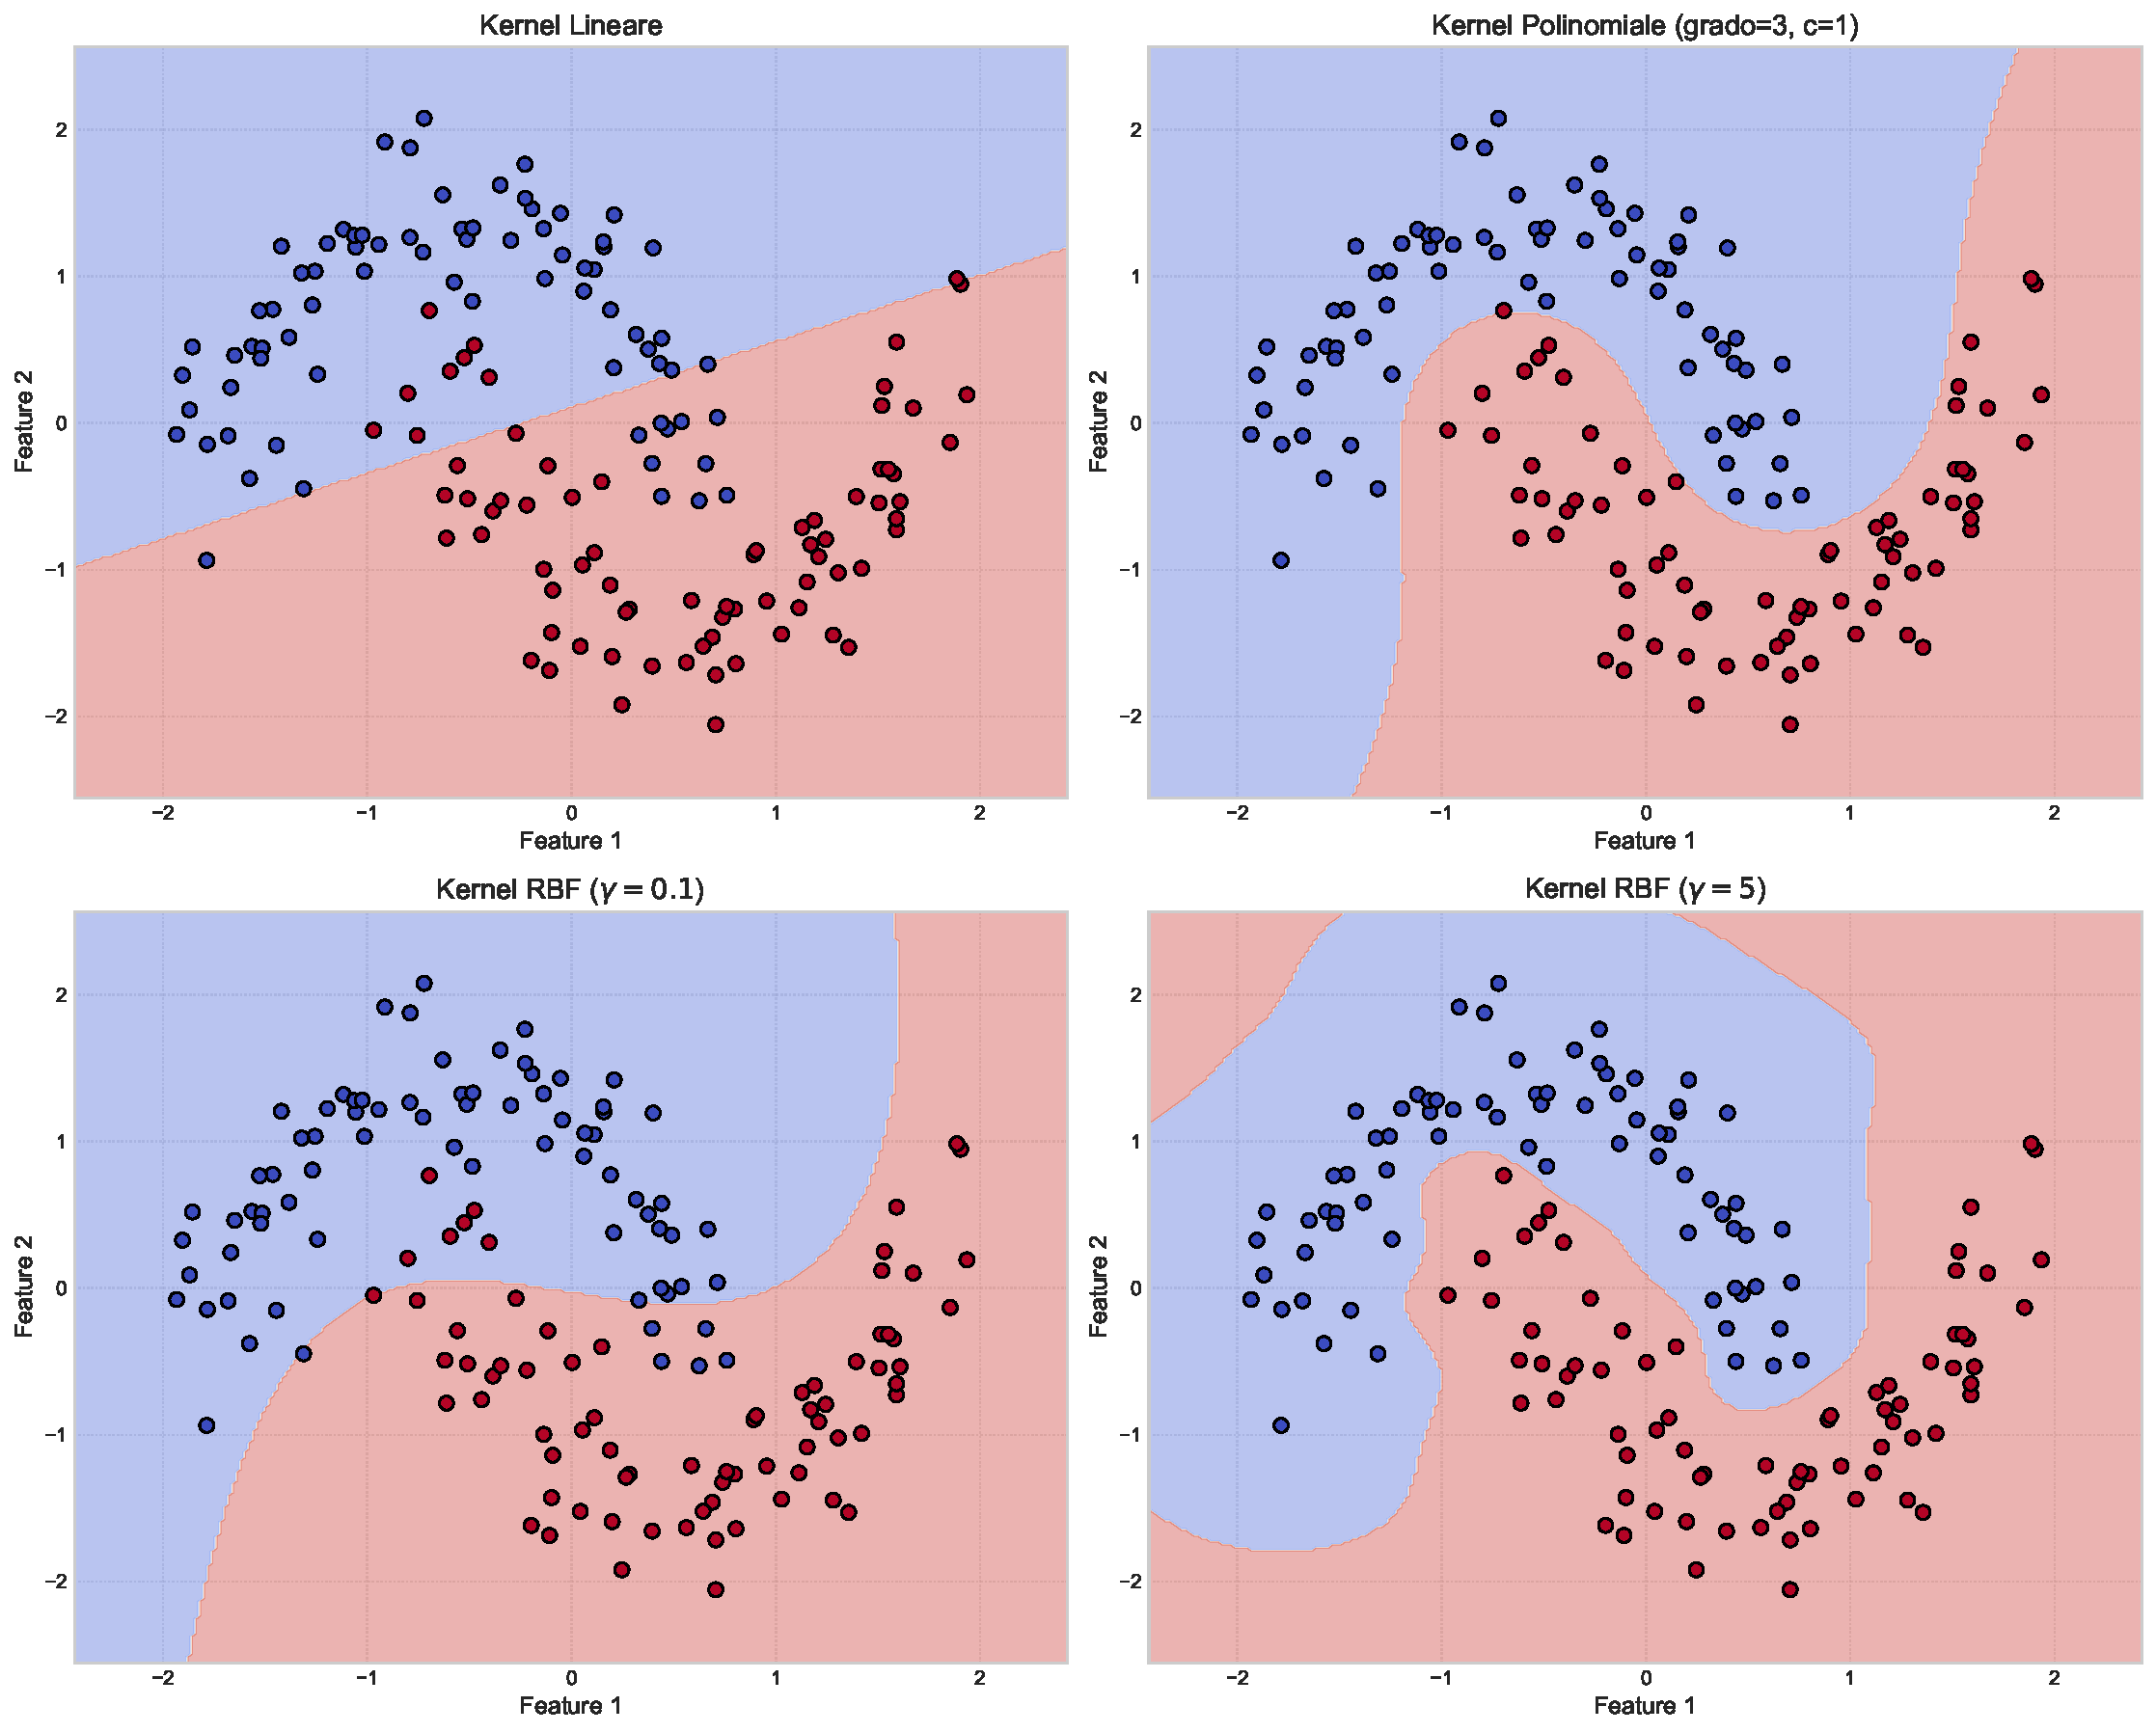
\includegraphics[width=\textwidth]{images/svm_kernel_examples.pdf}
    \caption{Esempi di confini di decisione ottenuti con SVM e diversi kernel (lineare, polinomiale, gaussiano con vari $\gamma$).}
    \label{fig:svm_kernel_examples}
\end{figure}

\paragraph{Iperparametri delle SVM con Kernel.}
La scelta del kernel e dei suoi iperparametri è cruciale per le prestazioni delle SVM.
\begin{itemize}
    \item Per il \textbf{kernel polinomiale}, gli iperparametri principali sono il grado $g$ e il coefficiente $C$ del margine soft. Aumentando il grado $g$ (con $C$ costante), aumenta la curvatura e la flessibilità del confine di decisione.
    \item Per il \textbf{kernel Gaussiano RBF}, gli iperparametri principali sono $\gamma$ e $C$.
          \begin{itemize}
              \item $\gamma$: Controlla l'influenza di un singolo esempio di training. Un $\gamma$ piccolo significa una gaussiana "larga", e i punti lontani influenzano il confine. Un $\gamma$ grande significa una gaussiana "stretta", e solo i punti vicini hanno un'influenza significativa, portando a confini più flessibili e potenzialmente all'overfitting.
              \item $C$: Come nel caso lineare, controlla il trade-off tra margine e errori di classificazione.
          \end{itemize}
          Lo spazio di ricerca per i parametri ottimali ($C$ e $g$, o $C$ e $\gamma$) è spesso bidimensionale e i valori vengono tipicamente variati su scala logaritmica. La combinazione ottimale viene scelta tramite cross-validation.
\end{itemize}

\begin{figure}[H]
    \centering
    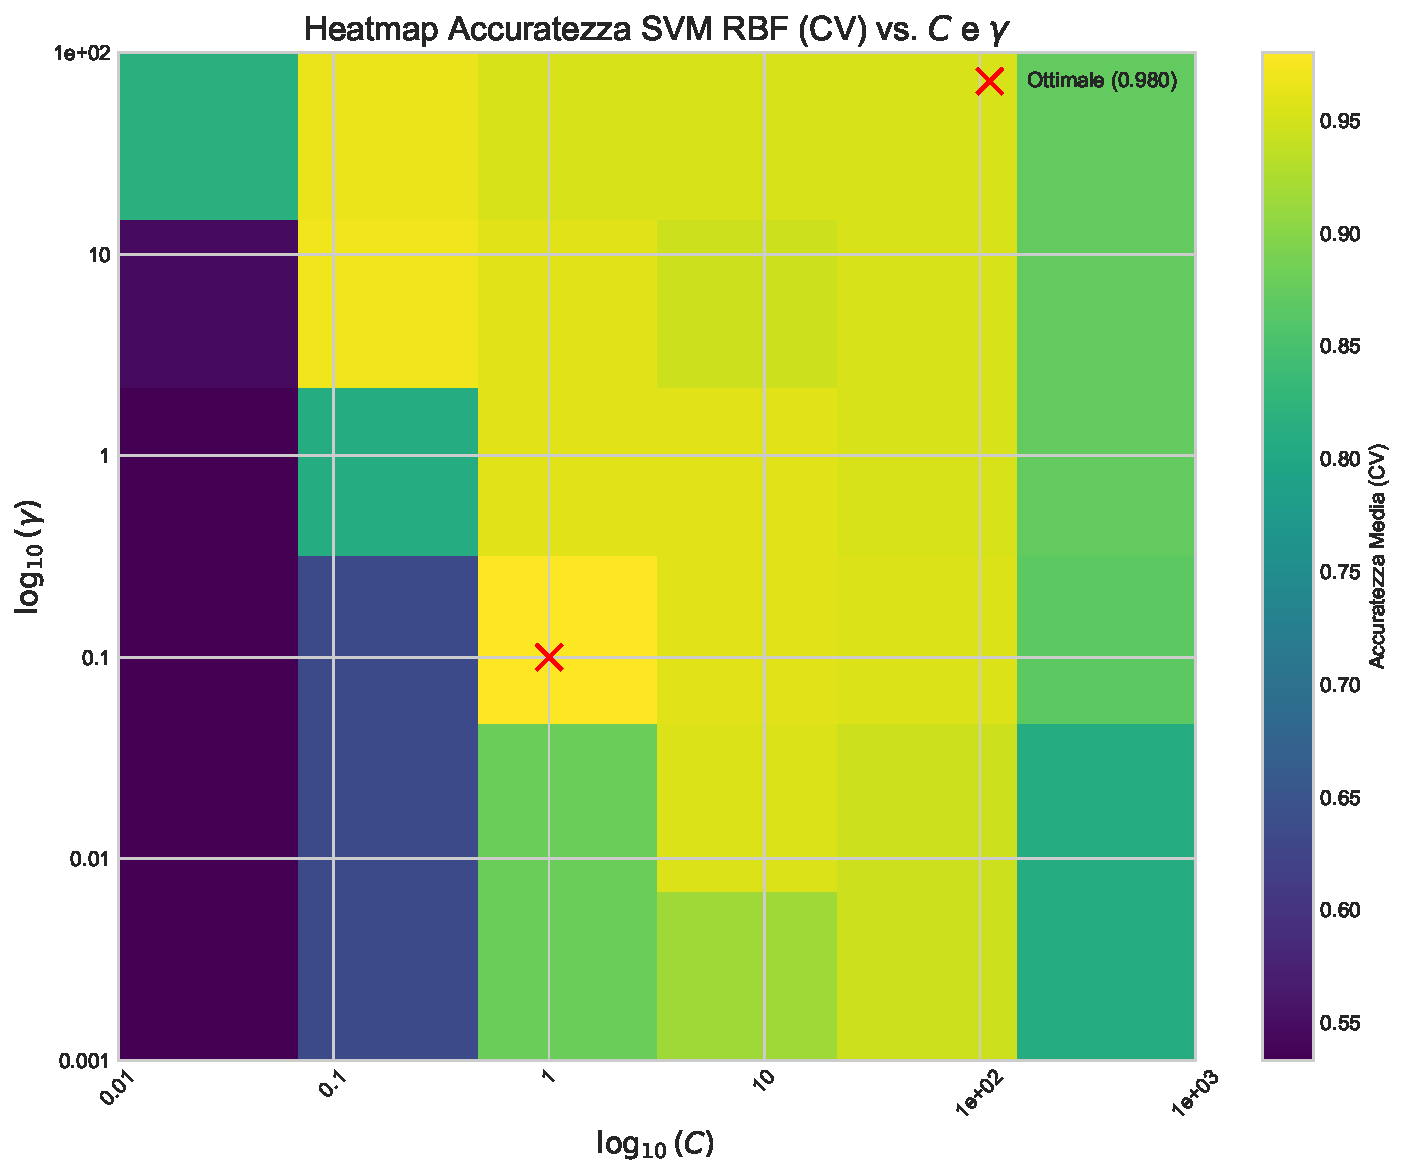
\includegraphics[width=0.7\textwidth]{images/svm_c_gamma_heatmap.pdf}
    \caption{Esempio di heatmap dell'accuratezza al variare degli iperparametri $C$ e $\gamma$ per un SVM con kernel RBF, utilizzata per trovare la combinazione ottimale.}
    \label{fig:svm_c_gamma_heatmap}
\end{figure}


\section{Alberi di Decisione per la Regressione}

Gli alberi di decisione possono essere utilizzati non solo per problemi di classificazione, ma anche per problemi di regressione, dove l'obiettivo è predire un valore continuo.

\subsection{Alberi di Regressione: Concetti di Base}
L'idea è di costruire una struttura ad albero dove:
\begin{itemize}
    \item Ogni \textbf{nodo intermedio} contiene un predicato (una condizione) basato su una delle variabili di input (feature). Questo predicato divide l'insieme delle istanze che arrivano al nodo in due (o più) sottoinsiemi, che vengono passati ai nodi figli.
    \item Ogni \textbf{nodo foglia} rappresenta una regione dello spazio delle feature e contiene un valore di predizione per la variabile di output $Y$. Questo valore è tipicamente la media dei valori di $Y$ di tutte le istanze di training che ricadono in quella foglia.
\end{itemize}
L'obiettivo durante la costruzione dell'albero è fare in modo che ogni nodo foglia contenga istanze con valori di $Y$ il più possibile simili tra loro, ovvero minimizzando l'errore di regressione (es. la somma dei quadrati dei residui) all'interno di ogni foglia.

\begin{figure}[H]
    \centering
    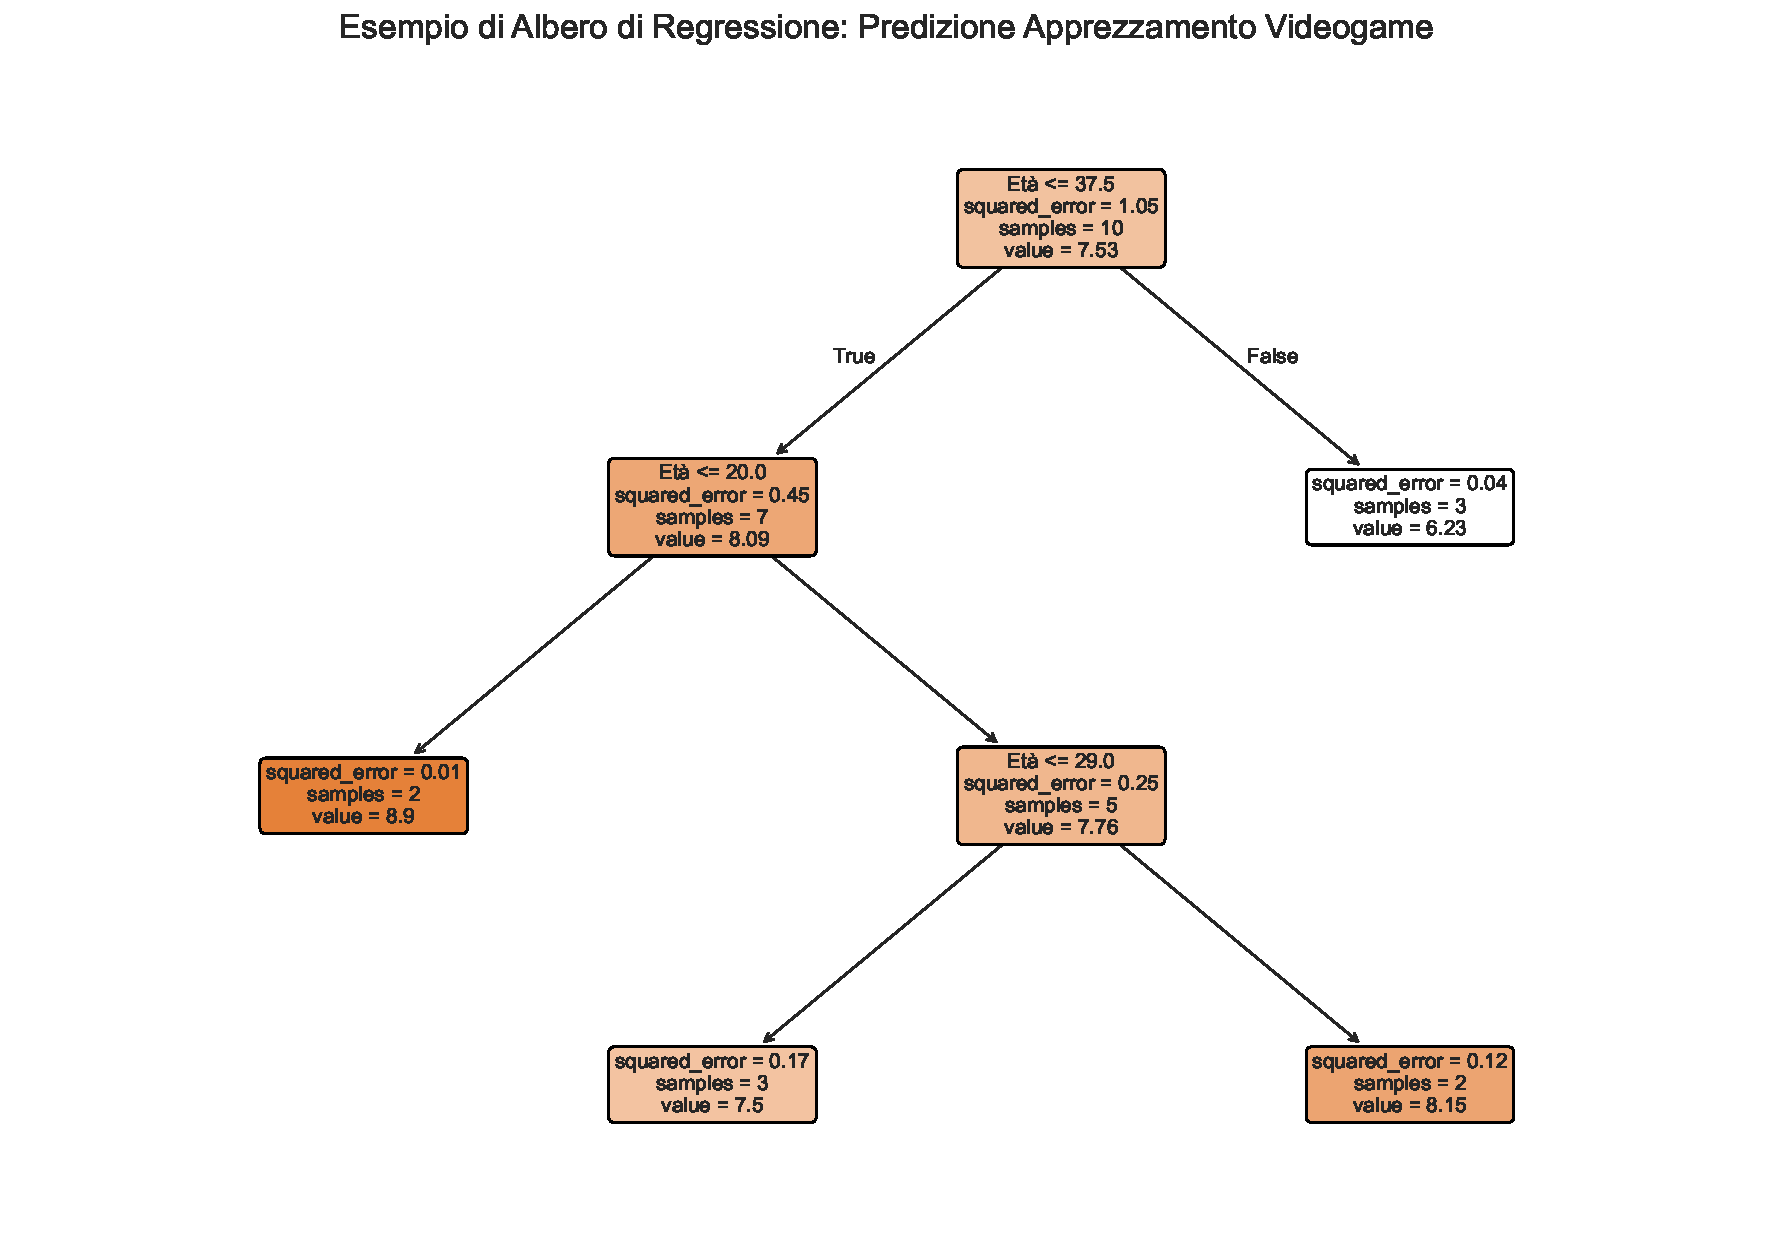
\includegraphics[width=1\textwidth]{images/regression_tree_example.pdf}
    \caption{Esempio di albero di regressione per predire l'apprezzamento dei videogame in base all'età e al genere. Le foglie contengono i punteggi di predizione.}
    \label{fig:regression_tree_example}
\end{figure}

\subsubsection{Costruzione dell'Albero: Divisione dello Spazio delle Feature}
La costruzione di un albero di regressione avviene tramite un processo ricorsivo di divisione (splitting) dello spazio delle feature.
\begin{enumerate}
    \item Si parte dal nodo radice, che contiene tutte le istanze di training.
    \item Per ogni nodo corrente, si cerca la migliore variabile di input e il miglior valore di soglia (split point) per dividere le istanze in due sottoinsiemi. "Migliore" significa che la divisione scelta è quella che porta alla massima riduzione dell'errore di regressione complessivo. Tipicamente, per ogni possibile split $(j, s)$ (variabile $j$ e valore di soglia $s$), si calcola l'errore quadratico medio (MSE) nei due sottoinsiemi risultanti ($R_1 = \{x | x_j < s\}$ e $R_2 = \{x | x_j \ge s\}$) rispetto alle medie $\hat{y}_{R_1}$ e $\hat{y}_{R_2}$ dei valori target in ciascun sottoinsieme:
          $$ \text{Errore}_{\text{split}} = \sum_{i \in R_1} (y_i - \hat{y}_{R_1})^2 + \sum_{i \in R_2} (y_i - \hat{y}_{R_2})^2 $$
          Si sceglie lo split $(j,s)$ che minimizza questo errore.
    \item Il processo di divisione continua ricorsivamente per ciascun nuovo nodo creato, fino a quando non si verifica una condizione di arresto.
\end{enumerate}
Questo processo partiziona lo spazio delle feature in regioni rettangolari (o iper-rettangolari in più dimensioni). All'interno di ogni regione (foglia), la predizione è costante e pari alla media dei valori $y$ delle istanze di training in quella regione.

\begin{figure}[H]
    \centering
    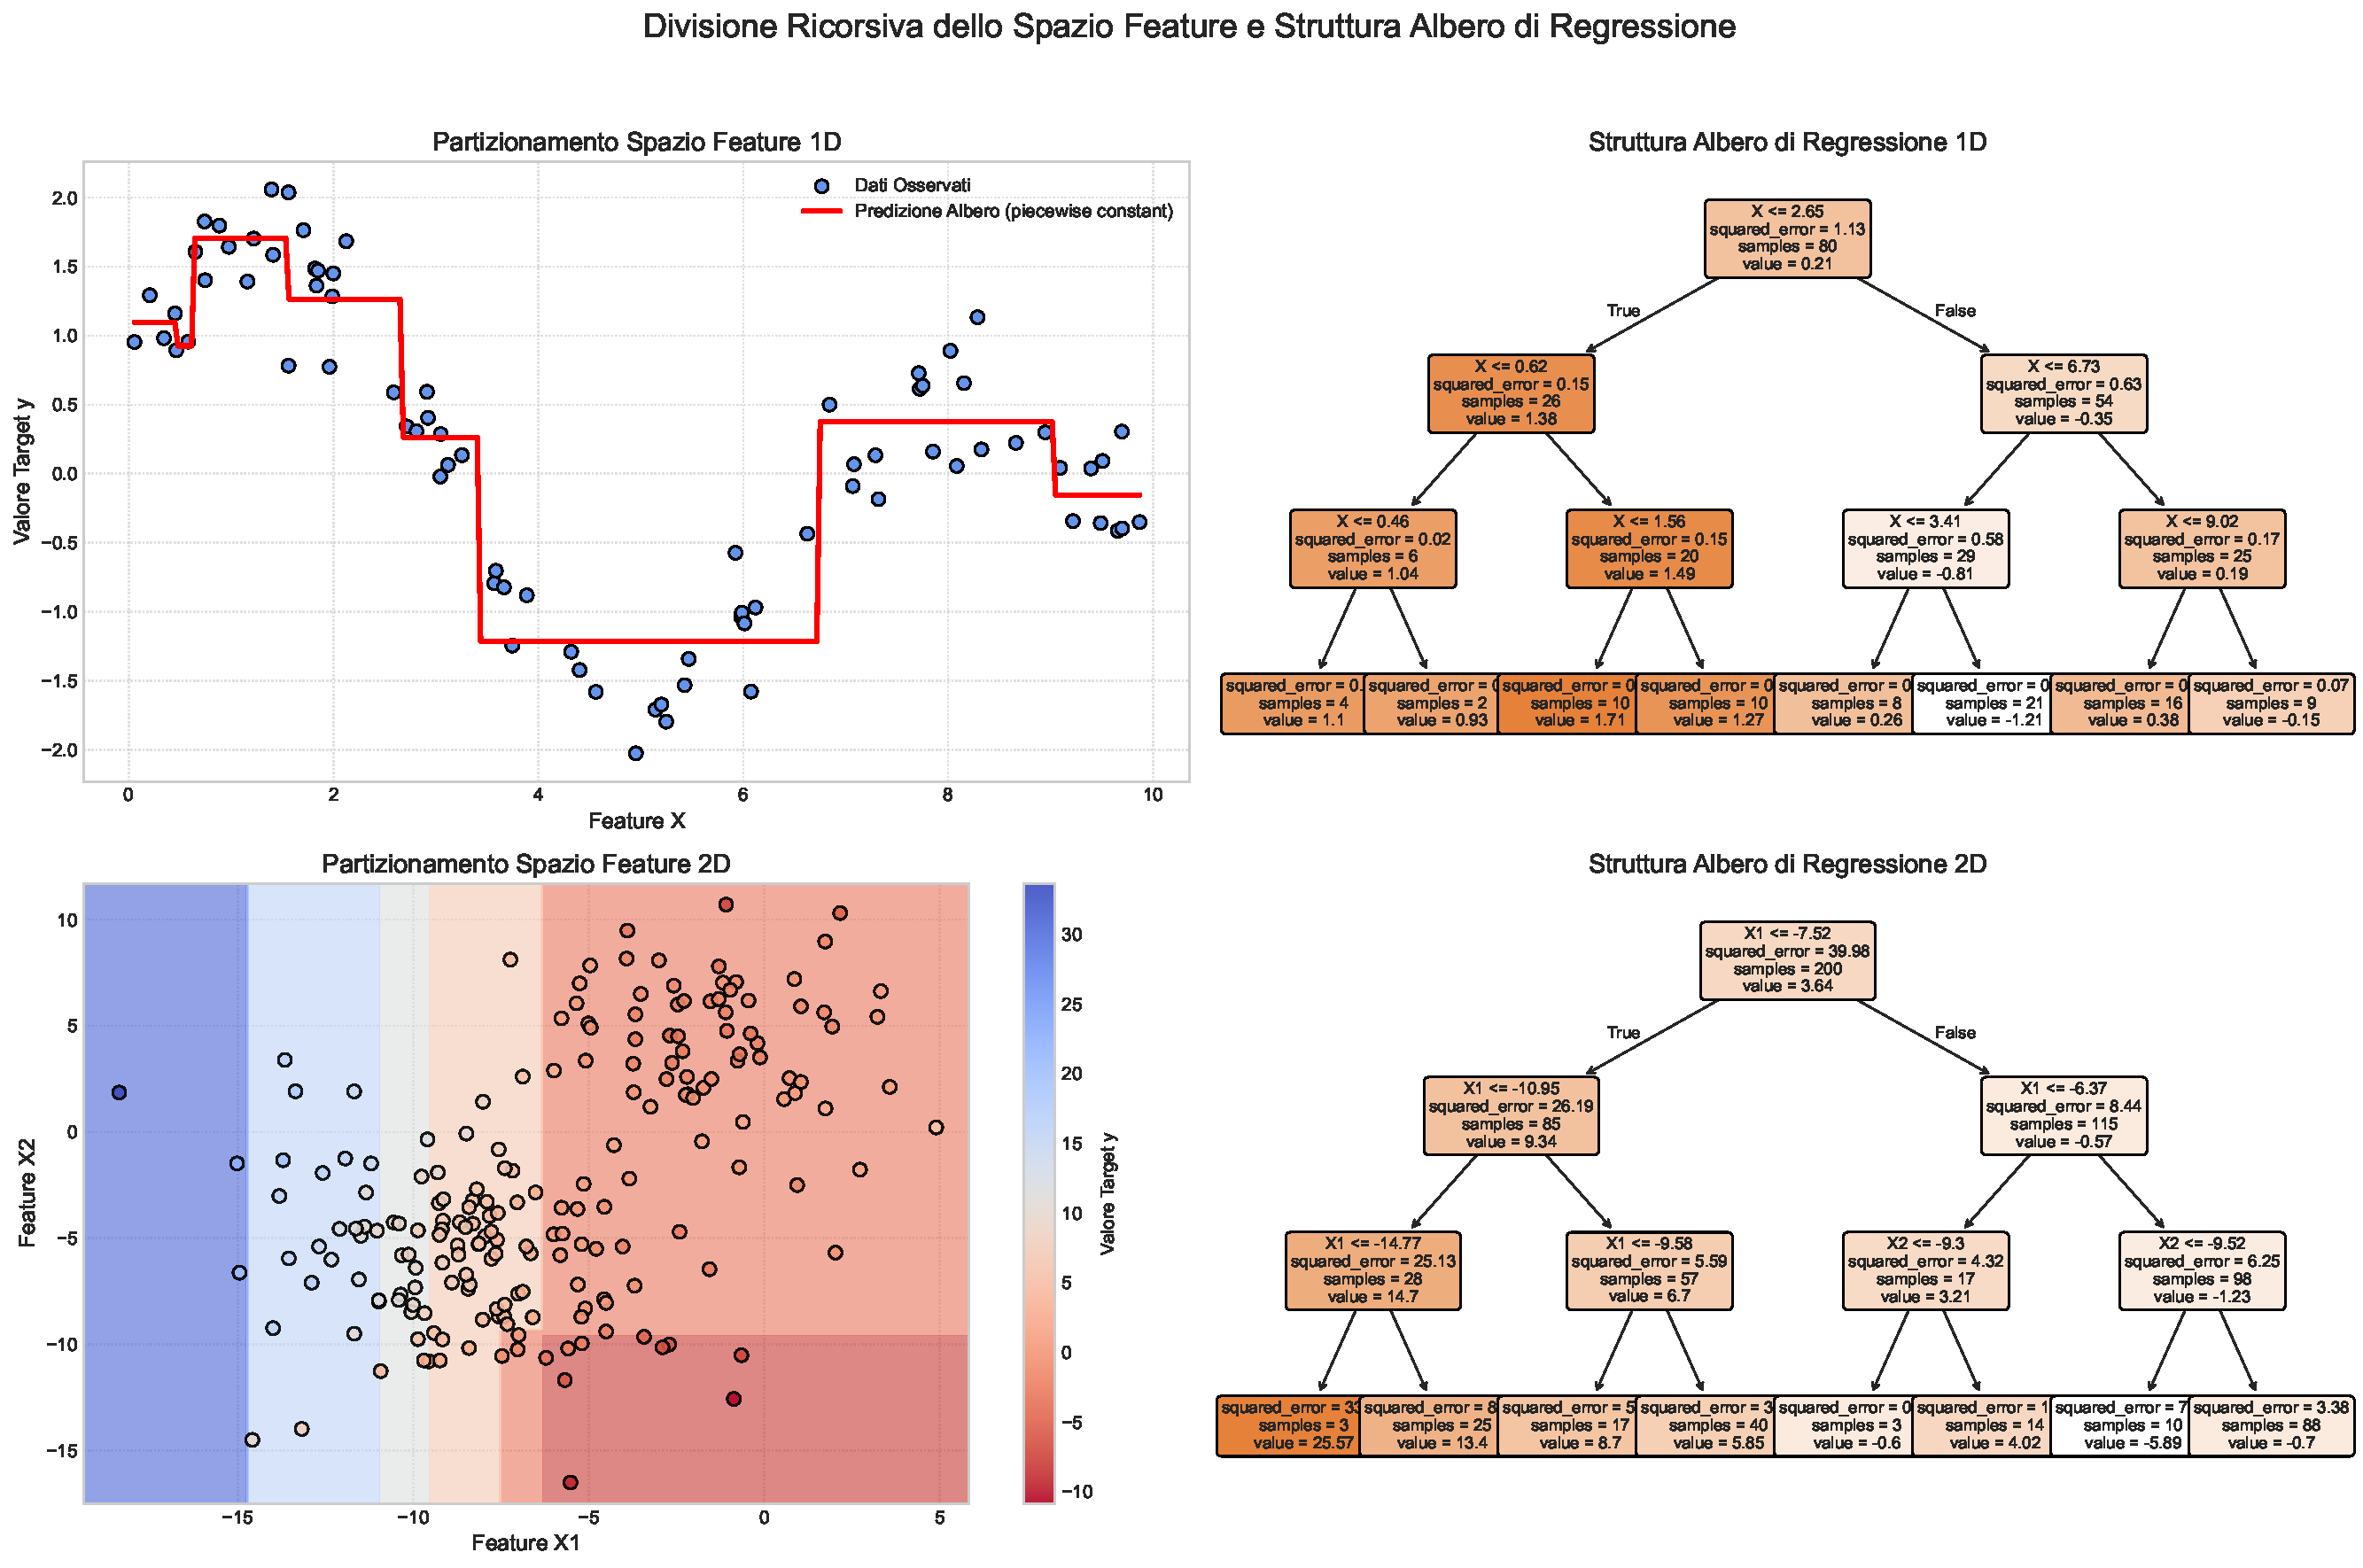
\includegraphics[width=1\textwidth]{images/feature_space_partitioning.pdf}
    \caption{Illustrazione della divisione ricorsiva dello spazio delle feature (in 1D e 2D) da parte di un albero di regressione e la corrispondente struttura ad albero.}
    \label{fig:feature_space_partitioning}
\end{figure}

\subsubsection{Algoritmo Greedy di Base per la Costruzione}
L'algoritmo tipico per costruire un albero di regressione è \textit{greedy} (ingordo), poiché ad ogni passo sceglie lo split che appare migliore localmente, senza garanzia di trovare l'albero globalmente ottimale.
Sia $S$ lo spazio (o sottoinsieme) corrente di istanze e $d$ il numero di variabili di input.
\begin{enumerate}
    \item Per ogni variabile di input $j=1, \dots, d$:
          \begin{enumerate}
              \item Per ogni possibile valore di separazione $v_j$ per la variabile $j$:
                    \begin{itemize}
                        \item Si dividono le istanze in $S$ in due sottoinsiemi: $S_{j,<} = \{i \in S | x_{i,j} < v_j\}$ e $S_{j,\ge} = \{i \in S | x_{i,j} \ge v_j\}$.
                        \item Si calcolano le medie dei valori target $\overline{y}_{<}$ e $\overline{y}_{\ge}$ per i due sottoinsiemi.
                        \item Si calcola l'MSE risultante per questo split: $\text{MSE}_{j,v_j} = \sum_{i \in S_{j,<}} (y_i - \overline{y}_{<})^2 + \sum_{i \in S_{j,\ge}} (y_i - \overline{y}_{\ge})^2$.
                    \end{itemize}
              \item Si sceglie il valore $v_j^*$ che minimizza $\text{MSE}_{j,v_j}$ per la variabile $j$.
          \end{enumerate}
    \item Si seleziona la variabile $p$ e il corrispondente valore di separazione $v_p^*$ che hanno prodotto l'MSE minimo assoluto tra tutti gli split testati.
    \item Se una condizione di stop non è soddisfatta:
          \begin{itemize}
              \item Si creano due nodi figli e si richiama ricorsivamente l'algoritmo sui sottoinsiemi $S_{p,<}$ e $S_{p,\ge}$.
          \end{itemize}
    \item Altrimenti (condizione di stop soddisfatta), il nodo corrente diventa una foglia e la predizione associata è la media dei valori $y$ delle istanze in $S$.
\end{enumerate}
Le \textbf{condizioni di stop} sono iperparametri e possono includere: massima profondità dell'albero, numero massimo di foglie, numero minimo di istanze per foglia, o un valore minimo di MSE al di sotto del quale non si divide più.

\subsubsection{Complessità del Modello, Overfitting e Potatura (Pruning)}
La complessità di un albero di regressione aumenta con la sua profondità (o dimensione). Un albero molto profondo può adattarsi molto bene ai dati di training, catturando anche il rumore, e quindi soffrire di \textbf{overfitting}, con scarse prestazioni su dati nuovi. È necessario regolare la complessità per bilanciare l'adattamento ai dati e la capacità di generalizzazione.
\begin{itemize}
    \item \textbf{Regolarizzazione}: Si può aggiungere un termine di penalizzazione alla funzione di costo (loss) che dipende dalla dimensione dell'albero (es. numero di foglie $T$):
          $$ \text{Loss}_{\text{reg}} = \text{ErroreDiTraining}(\text{Albero}) + C \times \text{Dimensione}(\text{Albero}) $$
          L'iperparametro $C$ (o $\alpha$) controlla il peso della penalizzazione e viene ottimizzato (es. con cross-validation).
    \item \textbf{Strategie di Creazione/Potatura}:
          \begin{itemize}
              \item \textit{Pre-pruning (arresto anticipato)}: L'albero viene fatto crescere, ma la divisione di un nodo viene fermata se non porta a un miglioramento sufficiente della loss (o se una condizione di stop è raggiunta).
              \item \textit{Post-pruning (potatura successiva)}: L'albero viene fatto crescere completamente (o quasi), e poi i rami che non contribuiscono significativamente alla generalizzazione (valutati ad esempio su un validation set) vengono potati (rimossi), partendo dalle foglie. Questa strategia è spesso preferita perché meno sensibile a scelte greedy non ottimali fatte durante la crescita.
          \end{itemize}
\end{itemize}

\paragraph{Regole di Potatura basate su Test Statistici.}
Una regola di stop o di post-pruning può essere basata su test statistici. Ad esempio, si può usare un \textbf{t-test di Student} per confrontare le medie dei valori $y$ nei due possibili nodi figli generati da uno split.
\begin{itemize}
    \item \textbf{Ipotesi Nulla ($H_0$)}: Le medie dei due gruppi di dati (corrispondenti ai due nodi figli) sono equivalenti.
    \item Si calcola il \textbf{t-score} (o t-value), che è il rapporto tra la differenza delle medie dei due gruppi e la variabilità interna a ciascun gruppo.
    \item Dal t-score e dai gradi di libertà, si calcola il \textbf{p-value}.
    \item Se il p-value è superiore a una soglia di significatività predefinita (es. $\alpha = 0.05$), si accetta l'ipotesi nulla, si considera la differenza tra i due gruppi come non statisticamente significativa (frutto del caso), e quindi lo split non viene effettuato (pre-pruning) o il sottoalbero viene potato (post-pruning), riunendo le due potenziali foglie in un unico nodo foglia.
\end{itemize}
Il t-score tra due gruppi $S_1$ (con media $\overline{y}_1$, varianza $\sigma_1^2$, numerosità $|S_1|$) e $S_2$ (con media $\overline{y}_2$, varianza $\sigma_2^2$, numerosità $|S_2|$) è dato da:
$$ t\text{-score} = \frac{\overline{y}_1 - \overline{y}_2}{\sqrt{\frac{\sigma_1^2}{|S_1|} + \frac{\sigma_2^2}{|S_2|}}} $$
Il p-value viene poi calcolato dalla distribuzione t di Student con $|S_1| + |S_2| - 2$ gradi di libertà.

\subsection{Foreste di Regressione (Ensemble Learning)}
Invece di utilizzare un singolo albero di decisione (per regressione o classificazione), si possono combinare le predizioni di più alberi per ottenere risultati generalmente migliori e più stabili. Questo approccio rientra nell'ambito dell'\textbf{Ensemble Learning}.
L'idea è che, combinando più modelli (alberi) semplici, si possa ridurre l'errore complessivo. Esistono diverse strategie per creare e combinare gli alberi:
\begin{itemize}
    \item \textbf{Bagging (Bootstrap Aggregating)}: Si creano molteplici alberi addestrandoli su diversi sottoinsiemi casuali dei dati di training (ottenuti con campionamento con reinserimento). Un esempio noto è l'algoritmo \textbf{Random Forest}, che introduce ulteriore casualità selezionando, per ogni split di ogni albero, solo un sottoinsieme casuale delle feature disponibili.
    \item \textbf{Boosting}: Gli alberi vengono costruiti in sequenza. Ogni nuovo albero cerca di correggere gli errori commessi dai modelli precedenti. Esempi includono \textbf{Gradient Boosting Machine (GBM)} e \textbf{XGBoost}.
\end{itemize}
L'output finale di una foresta di regressione è ottenuto combinando gli output dei singoli alberi, ad esempio tramite una media (per regressione) o un voto maggioritario (per classificazione). Sebbene l'uso di foreste aumenti la complessità computazionale e riduca l'interpretabilità diretta del singolo albero, spesso porta a un significativo miglioramento dell'accuratezza predittiva.

\begin{figure}[H]
    \centering
    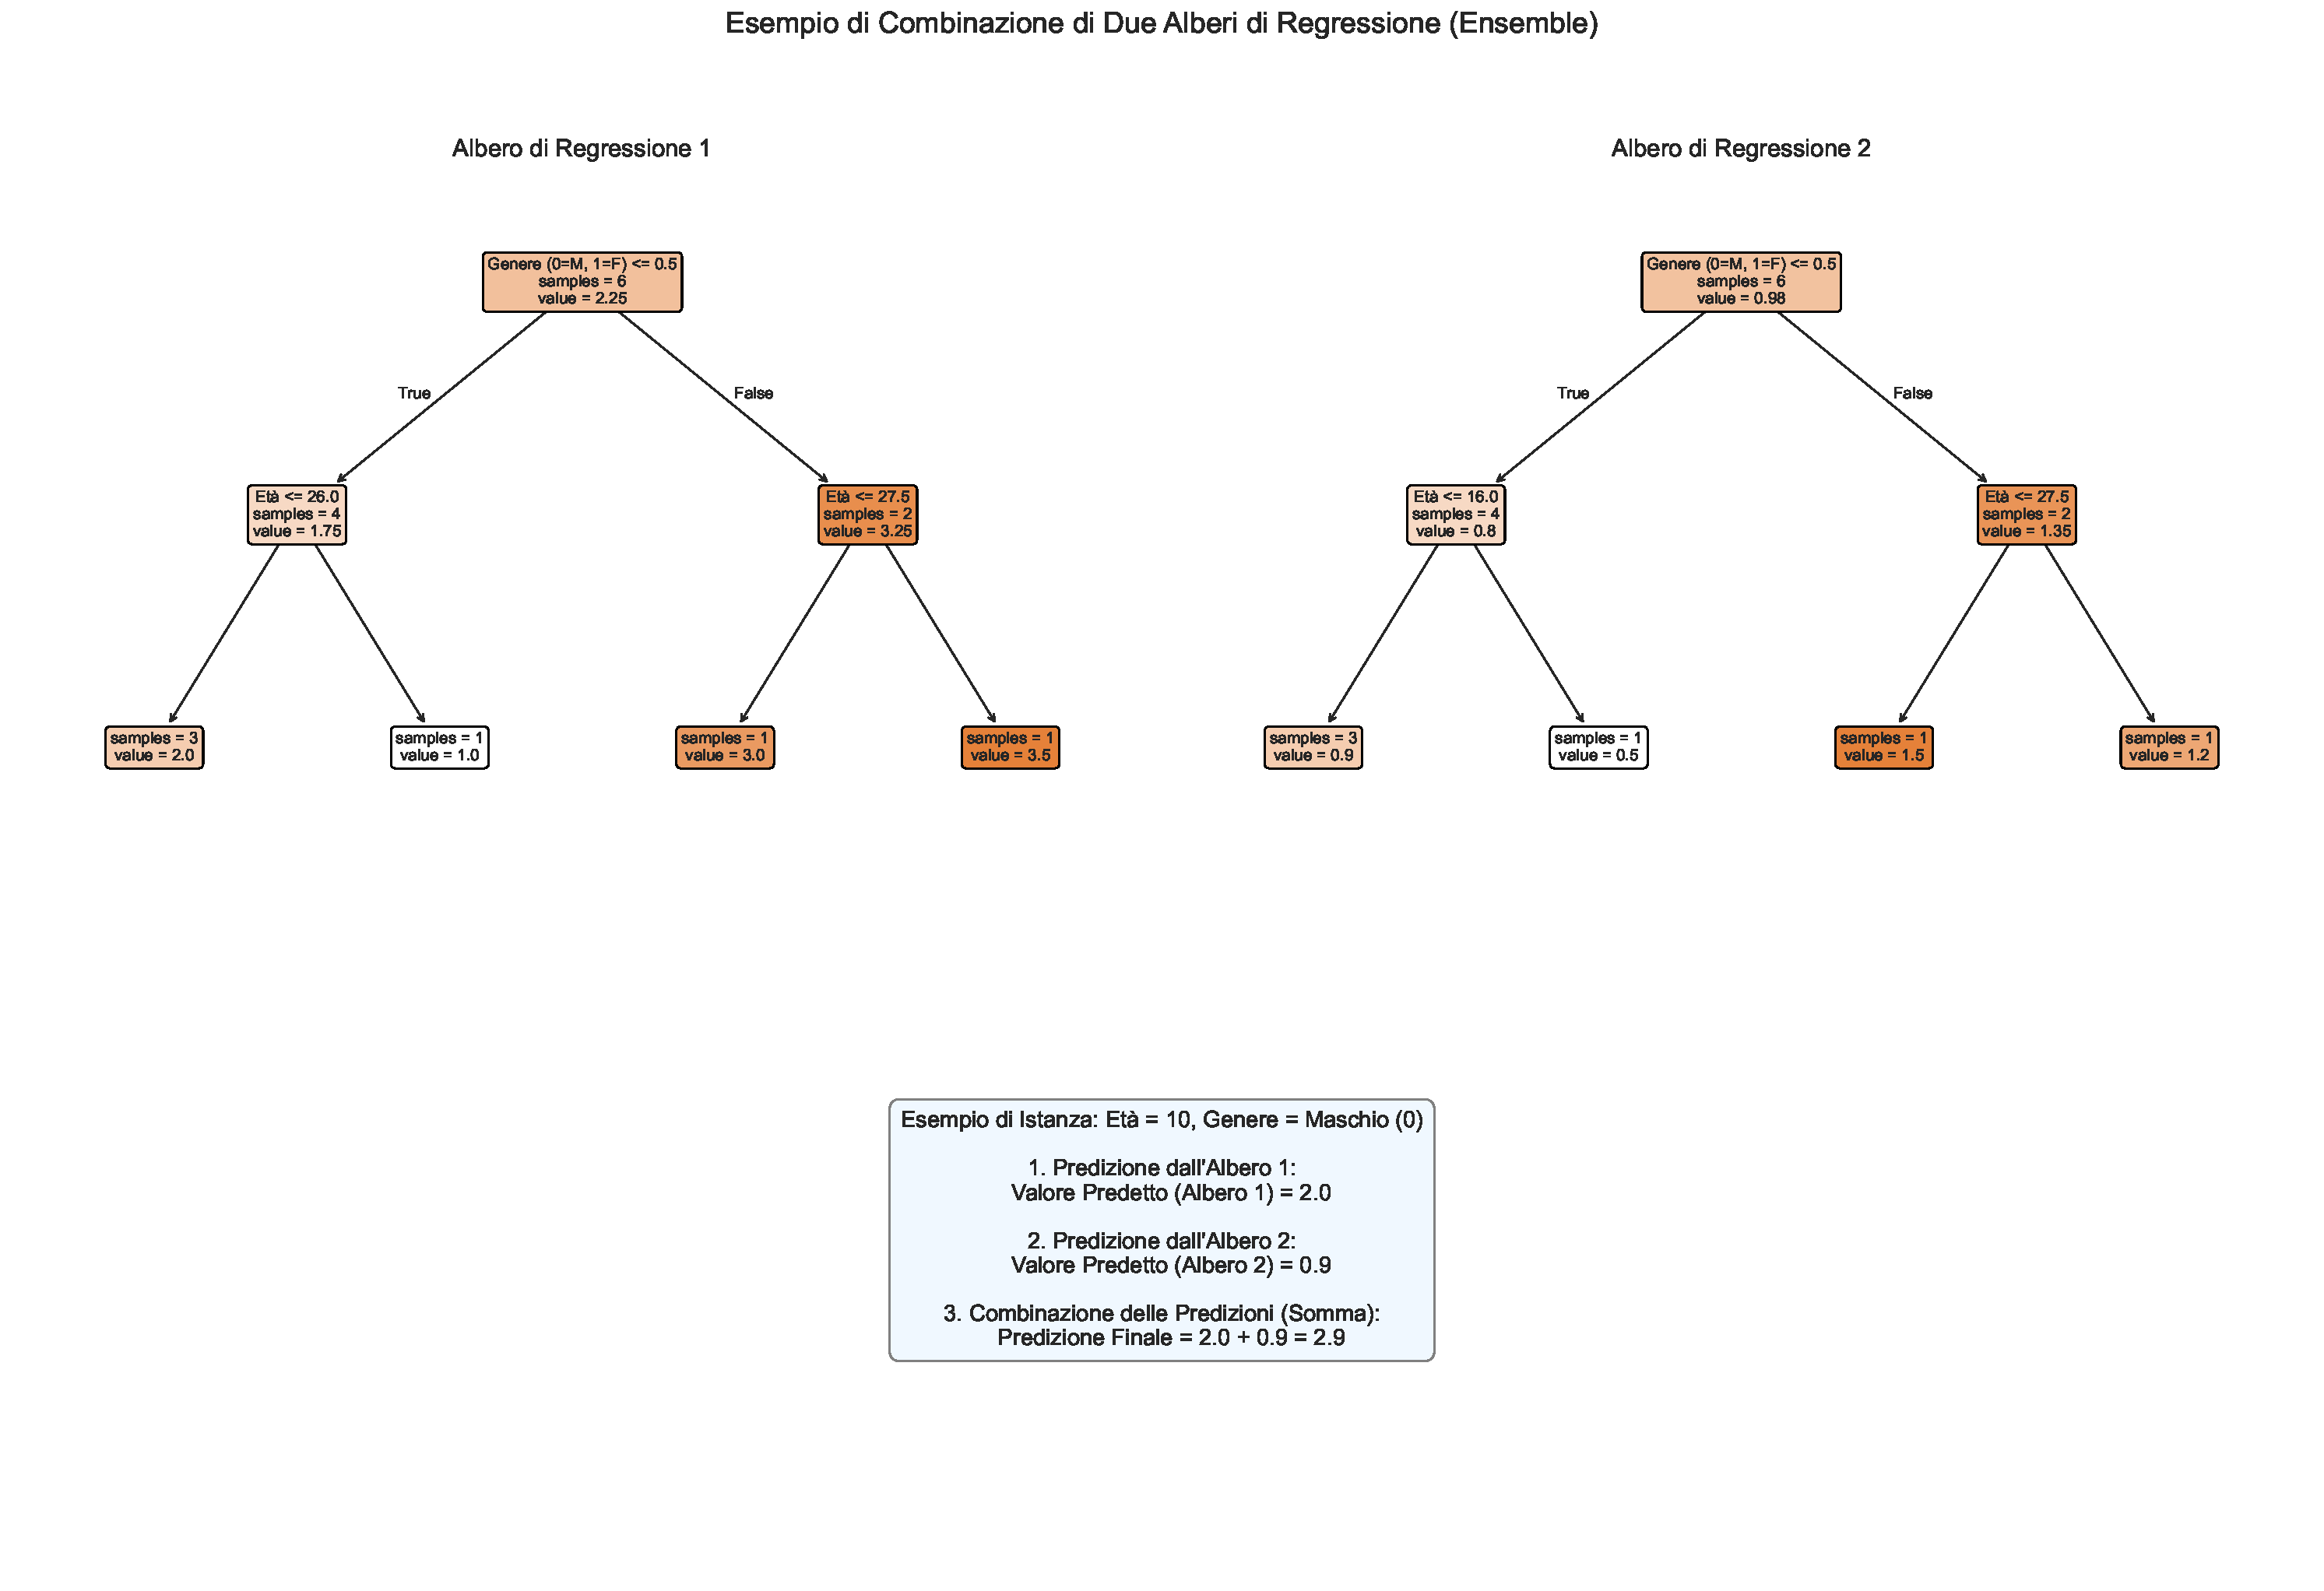
\includegraphics[width=1\textwidth]{images/ensemble_tree_example.pdf}
    \caption{Esempio di combinazione di due alberi di regressione. La previsione finale per un'istanza (es. un bambino maschio minore di 15 anni) è la somma dei valori predetti da ciascun albero (es. $2 + 0.9 = 2.9$).}
    \label{fig:ensemble_tree_example}
\end{figure}

\subsection{Gradient Boosting Machine (GBM)}
Il Gradient Boosting è una tecnica di ensemble learning che costruisce modelli in modo additivo e sequenziale.

\subsubsection{Learning Additivo di Più Modelli}
Si inizia con un modello base semplice, spesso una previsione costante (es. la media dei valori target, o zero). Ad ogni iterazione $t$, si aggiunge un nuovo modello $f_t(x_i)$ al modello complessivo costruito fino all'iterazione precedente $\hat{y}_i^{(t-1)}$:
$$ \hat{y}_i^{(0)} = \text{costante (es. 0)} $$
$$ \hat{y}_i^{(1)} = \hat{y}_i^{(0)} + f_1(x_i) $$
$$ \hat{y}_i^{(2)} = \hat{y}_i^{(1)} + f_2(x_i) = f_1(x_i) + f_2(x_i) $$
$$ \dots $$
$$ \hat{y}_i^{(t)} = \sum_{k=1}^{t} f_k(x_i) = \hat{y}_i^{(t-1)} + f_t(x_i) $$
Ogni nuovo albero $f_t(x_i)$ viene addestrato per predire gli \textbf{errori residui} del modello precedente, ovvero le differenze $y_i - \hat{y}_i^{(t-1)}$ tra i valori reali $y_i$ e le predizioni del modello fino a quel punto $\hat{y}_i^{(t-1)}$.

La funzione di perdita (Loss) da minimizzare per l'intero ensemble di $N$ istanze, ad esempio utilizzando l'Errore Quadratico Medio (MSE), è:
$$ L(y, \hat{y}^{(t)}) = \frac{1}{N} \sum_{i=1}^{N} (y_i - \hat{y}_i^{(t)})^2 $$

\subsubsection{Gradient Boosting e Discesa del Gradiente}
Esiste una forte analogia tra il Gradient Boosting e l'algoritmo della discesa del gradiente. L'obiettivo è minimizzare la funzione di perdita $L(y, \hat{y}^{(t)})$. La derivata parziale della loss MSE rispetto alla predizione $\hat{y}_j^{(t)}$ per una singola istanza $j$ (eliminando costanti e la sommatoria per la derivata rispetto a una singola predizione) è:
$$ \frac{\partial L(y_j, \hat{y}_j^{(t)})}{\partial \hat{y}_j^{(t)}} = \frac{\partial (y_j - \hat{y}_j^{(t)})^2}{\partial \hat{y}_j^{(t)}} = -2(y_j - \hat{y}_j^{(t)}) $$
Il gradiente (o meglio, il negativo del gradiente, che è il residuo $y_j - \hat{y}_j^{(t)}$, a meno di una costante) indica la direzione in cui la loss diminuisce più rapidamente.
Il modello GBM è una funzione ricorrente $\hat{y}^{(t)} = \hat{y}^{(t-1)} + f_t(x)$. L'aggiunta di un nuovo modello $f_t(x)$ ad ogni iterazione $t$ ha lo scopo di ridurre il residuo (cioè, muoversi nella direzione opposta al gradiente della loss). Infatti, l'aggiornamento del modello può essere visto come un passo della discesa del gradiente nello spazio delle funzioni, dove il nuovo modello $f_t(x)$ è scelto per approssimare il negativo del gradiente della loss rispetto alle predizioni del modello precedente $\hat{y}^{(t-1)}$. Introducendo un tasso di apprendimento (learning rate) $\eta$:
$$ \hat{y}^{(t)} \approx \hat{y}^{(t-1)} + \eta \cdot (\text{modello che approssima } - \nabla L(y, \hat{y}^{(t-1)})) $$
Nel caso della MSE, $- \nabla L(y_j, \hat{y}_j^{(t-1)})$ è proporzionale a $y_j - \hat{y}_j^{(t-1)}$, quindi $f_t(x)$ viene addestrato sui residui.

\begin{figure}[H]
    \centering
    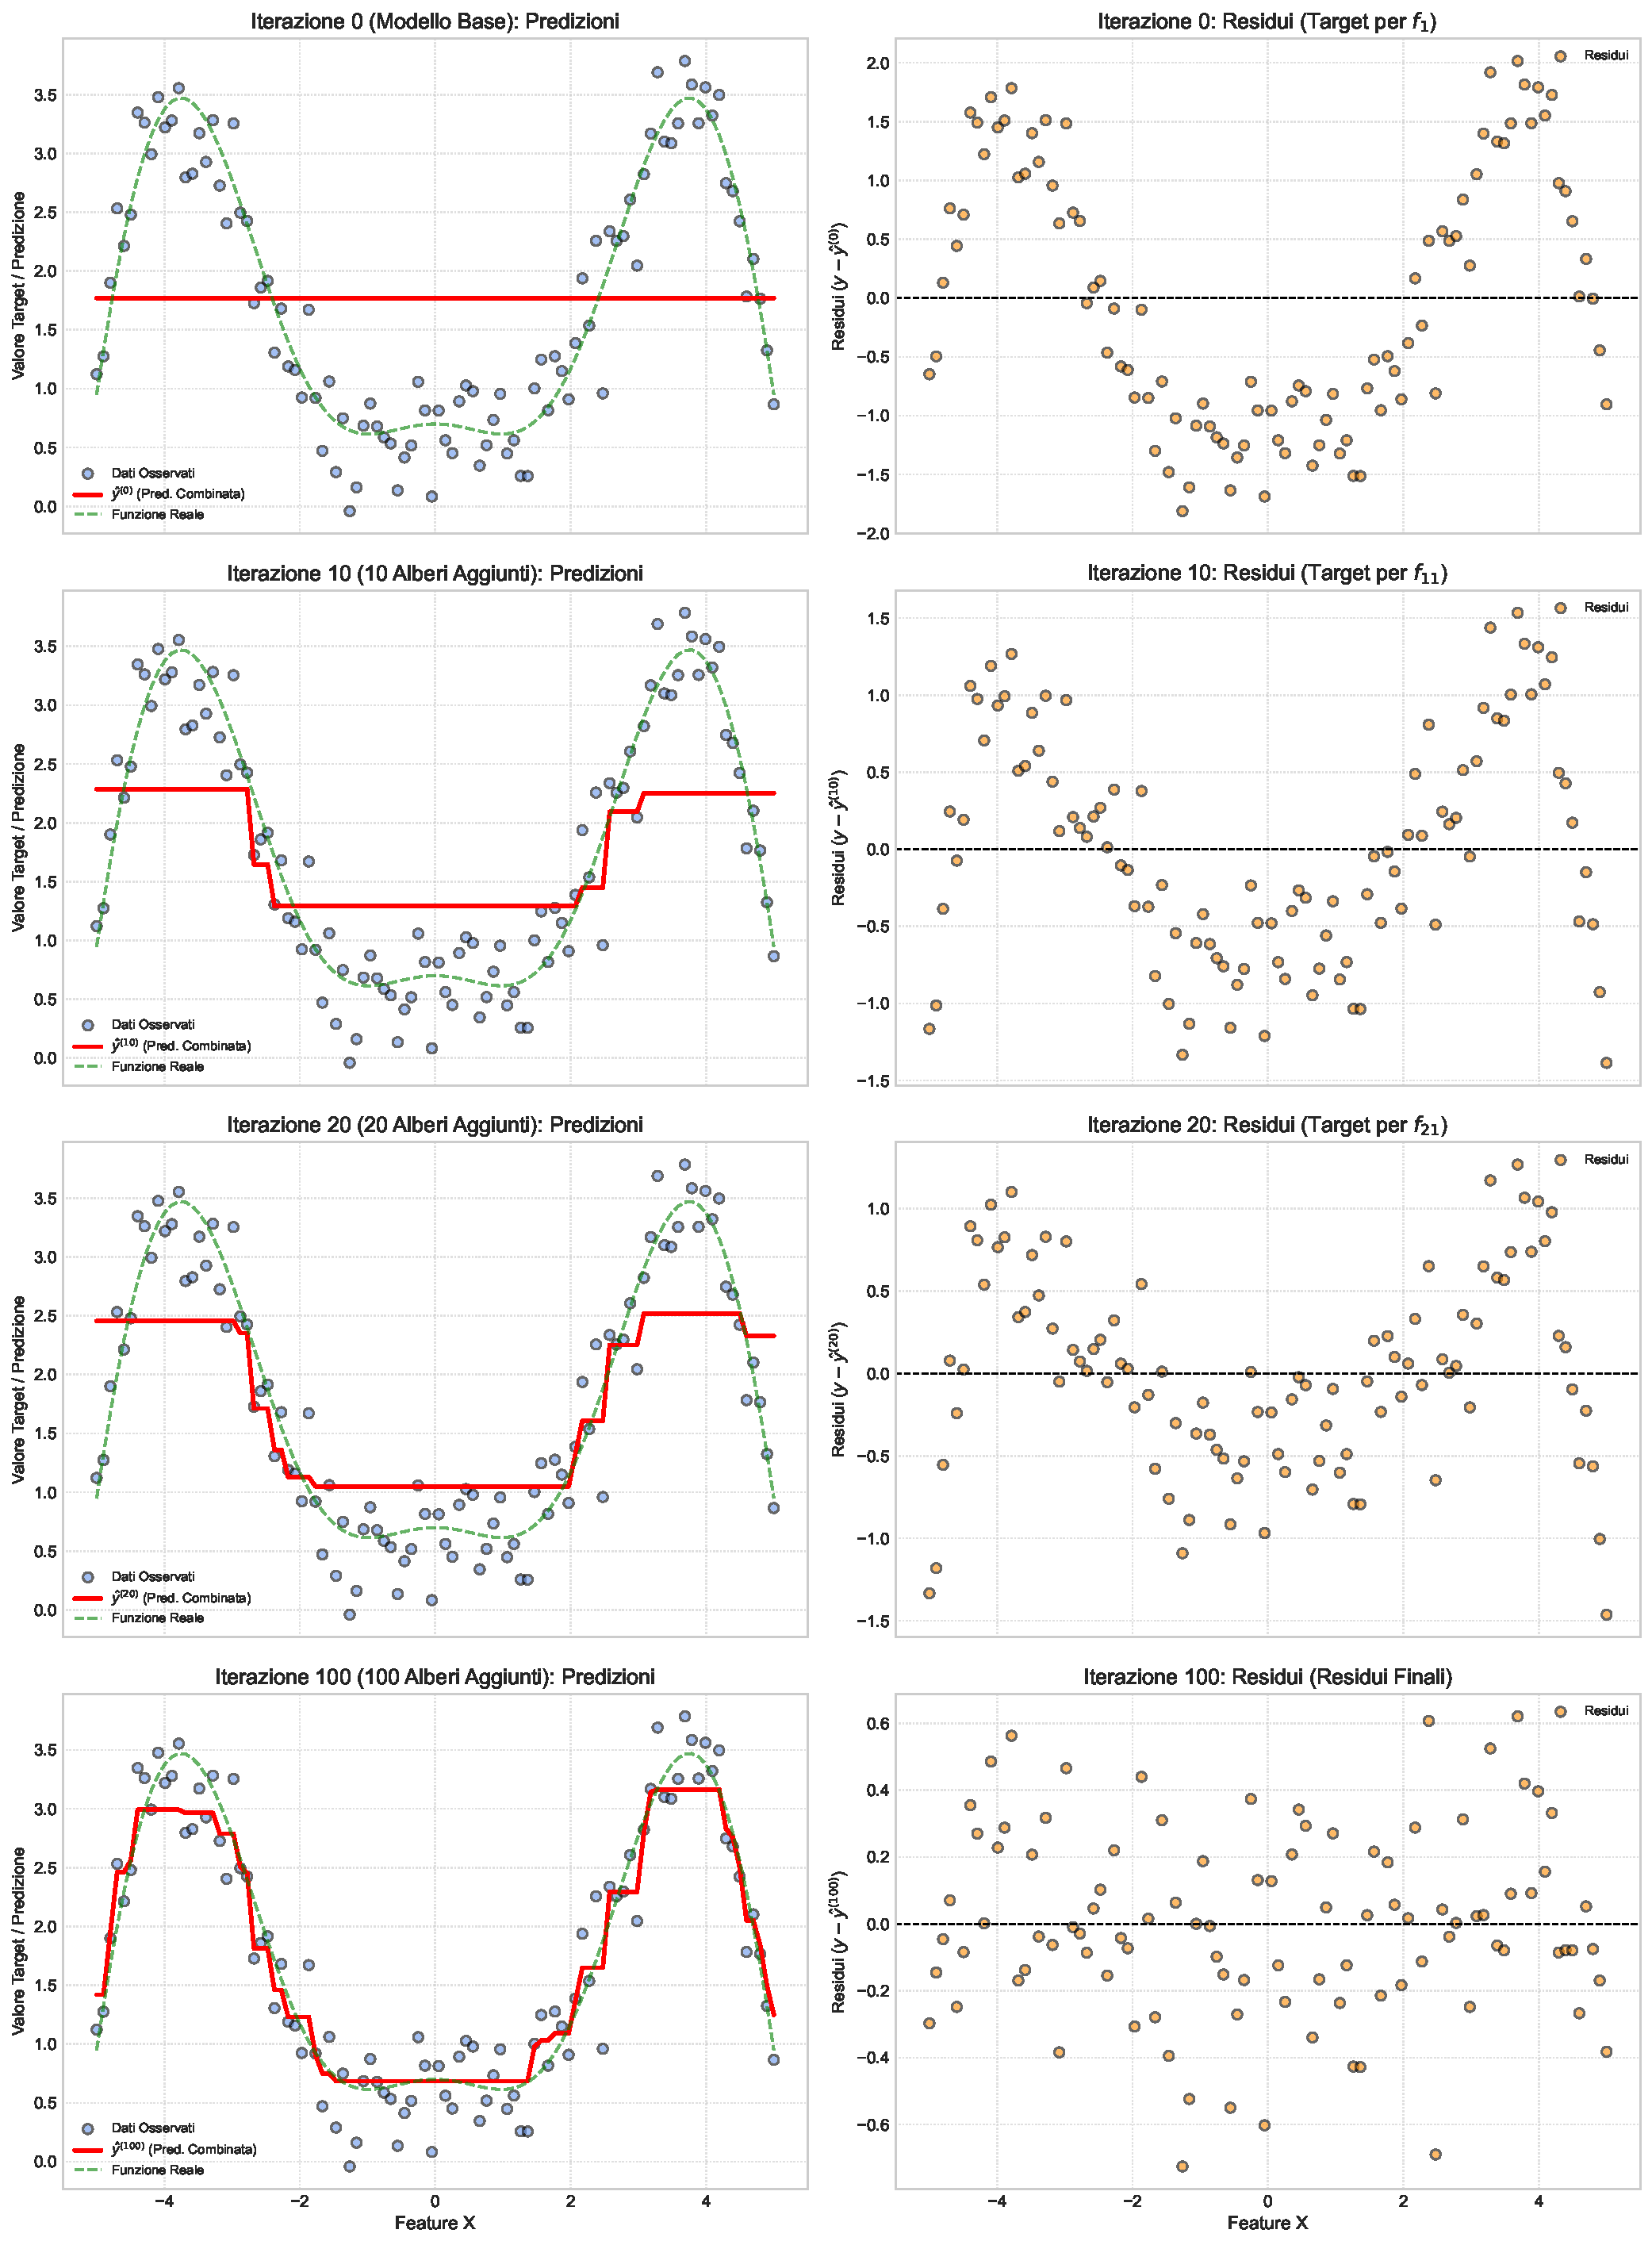
\includegraphics[width=\textwidth]{images/gbm_iterations_example.pdf}
    \caption{Esempio di iterazioni del Gradient Boosting. Ad ogni passo, un nuovo albero viene addestrato sui residui del modello precedente. Inizialmente (iterazione 0), la predizione è una costante (es. media) e i residui sono le differenze originali. Con il progredire delle iterazioni, la predizione combinata (linea rossa) si adatta meglio ai dati (punti blu) e i residui tendono a distribuirsi casualmente attorno allo zero.}
    \label{fig:gbm_iterations}
\end{figure}

\subsection{Funzione Obiettivo nel Supervised Learning Additivo (Contesto XGBoost)}
Per un singolo modello parametrico (es. regressione lineare con parametri $w_j$), l'obiettivo del supervised learning è determinare i parametri $\Theta = \{w_j\}$ che minimizzano una funzione obiettivo:
$$ Obj(\Theta) = L(\Theta) + \Omega(\Theta) $$
dove $L(\Theta) = \sum_{i} (f(x_i) - y_i)^2$ è la loss (es. somma dei quadrati degli errori, o SSE) che misura l'errore sul training set, e $\Omega(\Theta) = \lambda ||w||_2^2$ è un termine di regolarizzazione (es. L2) che penalizza la complessità del modello per prevenire l'overfitting.

Quando si apprendono $K$ alberi in un modello additivo come $\hat{y}_i = \sum_{k=1}^{K} f_k(x_i)$, dove ogni $f_k$ è un albero, la funzione obiettivo diventa:
$$ Obj = \sum_{i=1}^{n} l(y_i, \hat{y}_i) + \sum_{k=1}^{K} \Omega(f_k) $$
Qui, $l(y_i, \hat{y}_i)$ è la loss per la singola istanza $i$ (es. $(y_i - \hat{y}_i)^2$), e $\Omega(f_k)$ è un termine che misura la complessità del $k$-esimo albero. La minimizzazione della loss $l$ riduce l'errore sul training set, mentre la regolarizzazione $\Omega$ controlla la complessità degli alberi per migliorare la generalizzazione.

\subsubsection{Regolarizzazione e Definizione della Complessità di un Albero (XGBoost)}
La complessità di un albero di regressione $f_t(x)$ è data dalla sua struttura (numero di foglie, profondità) e dai valori predetti nelle foglie. XGBoost definisce la complessità di un singolo albero $f_t$ come:
$$ \Omega(f_t) = \gamma T + \frac{1}{2} \lambda \sum_{j=1}^{T} w_j^2 $$
Dove:
\begin{itemize}
    \item $T$ è il numero di foglie dell'albero $f_t$.
    \item $w_j$ è il punteggio (valore di regressione) predetto nella $j$-esima foglia.
    \item $\gamma$ è un iperparametro che penalizza il numero di foglie (controlla la potatura).
    \item $\lambda$ è un iperparametro che applica una regolarizzazione L2 sui punteggi delle foglie, simile alla Ridge Regression, per evitare che i valori predetti diventino troppo grandi.
\end{itemize}
Ad esempio, per un albero con $T=3$ foglie e punteggi $w_1=2, w_2=0.1, w_3=-1$, la complessità sarebbe $\Omega = 3\gamma + \frac{1}{2}\lambda(2^2 + 0.1^2 + (-1)^2) = 3\gamma + \frac{1}{2}\lambda(5.01)$.

\subsubsection{XGBoost: Apprendimento Additivo e Funzione Obiettivo}
XGBoost (Extreme Gradient Boosting) apprende gli alberi in modo additivo, come il GBM. All'iterazione $t$, si vuole trovare un albero $f_t(x_i)$ che ottimizzi la funzione obiettivo. La predizione all'iterazione $t$ è $\hat{y}_i^{(t)} = \hat{y}_i^{(t-1)} + f_t(x_i)$. La funzione obiettivo all'iterazione $t$ può essere scritta come:
$$ Obj^{(t)} = \sum_{i=1}^{n} l(y_i, \hat{y}_i^{(t-1)} + f_t(x_i)) + \Omega(f_t) + \text{costante} $$
dove la costante raggruppa i termini di regolarizzazione degli alberi precedenti $\sum_{k=1}^{t-1} \Omega(f_k)$, che non dipendono da $f_t$.
Per ottimizzare questa funzione rispetto a $f_t$, XGBoost utilizza un'approssimazione di Taylor del secondo ordine per la funzione di loss $l(y_i, \hat{y}_i^{(t-1)} + f_t(x_i))$ attorno a $\hat{y}_i^{(t-1)}$:
$$ l(y_i, \hat{y}_i^{(t-1)} + f_t(x_i)) \approx l(y_i, \hat{y}_i^{(t-1)}) + g_i f_t(x_i) + \frac{1}{2} h_i f_t^2(x_i) $$
dove $g_i = \frac{\partial l(y_i, \hat{y})}{\partial \hat{y}} \Big|_{\hat{y}=\hat{y}_i^{(t-1)}}$ è la derivata prima (gradiente) della loss rispetto alla predizione del passo precedente, e $h_i = \frac{\partial^2 l(y_i, \hat{y})}{\partial \hat{y}^2} \Big|_{\hat{y}=\hat{y}_i^{(t-1)}}$ è la derivata seconda (Hessiana).
Per la loss MSE, $l(y_i, \hat{y}_i) = (\hat{y}_i - y_i)^2$, si ha $g_i = 2(\hat{y}_i^{(t-1)} - y_i)$ e $h_i = 2$.

Sostituendo l'approssimazione di Taylor e rimuovendo i termini costanti (che non dipendono da $f_t(x_i)$), la funzione obiettivo da minimizzare per trovare $f_t$ diventa approssimativamente:
$$ Obj^{(t)} \approx \sum_{i=1}^{n} [g_i f_t(x_i) + \frac{1}{2} h_i f_t^2(x_i)] + \Omega(f_t) $$
Sostituendo $\Omega(f_t) = \gamma T + \frac{1}{2} \lambda \sum_{j=1}^{T} w_j^2$ e raggruppando i termini per foglia (dove $f_t(x_i) = w_{q(x_i)}$ è il punteggio della foglia $q(x_i)$ a cui appartiene l'istanza $x_i$, e $I_j$ è l'insieme delle istanze nella foglia $j$):
$$ Obj^{(t)} \approx \sum_{j=1}^{T} \left[ \left(\sum_{i \in I_j} g_i\right) w_j + \frac{1}{2} \left(\sum_{i \in I_j} h_i + \lambda\right) w_j^2 \right] + \gamma T $$
Definendo $G_j = \sum_{i \in I_j} g_i$ e $H_j = \sum_{i \in I_j} h_i$, l'obiettivo è una somma di $T$ funzioni quadratiche indipendenti, una per ogni foglia. Per una data struttura d'albero (cioè, per un dato partizionamento in foglie $I_j$), il punteggio ottimale $w_j^*$ per ciascuna foglia $j$ che minimizza questa espressione è:
$$ w_j^* = - \frac{G_j}{H_j + \lambda} $$
E il valore ottimale della funzione obiettivo (senza $\gamma T$ per ora) per quella struttura d'albero è:
$$ Obj^* = - \frac{1}{2} \sum_{j=1}^{T} \frac{G_j^2}{H_j + \lambda} $$
Aggiungendo il termine di penalizzazione per il numero di foglie, si ottiene il valore complessivo $Obj^* + \gamma T$. Minore è questo valore, migliore è la struttura dell'albero.

\subsubsection{Algoritmo di Ricerca Greedy della Struttura dell'Albero in XGBoost}
La ricerca della struttura ottimale dell'albero (cioè, quali split fare) è un problema complesso. XGBoost utilizza un algoritmo greedy:
\begin{enumerate}
    \item Si inizia da un albero con una singola foglia (profondità zero).
    \item Per ogni nodo foglia esistente, si prova iterativamente ad aggiungere uno split su una delle feature. Per ogni possibile split (feature e valore di soglia):
          \begin{itemize}
              \item Si calcolano $G_L, H_L$ per il nodo figlio sinistro proposto e $G_R, H_R$ per il nodo figlio destro proposto.
              \item Si calcola il \textbf{guadagno (Gain)} ottenuto dallo split come la riduzione nella funzione obiettivo:
                    $$ \text{Gain} = \left( \frac{G_L^2}{H_L+\lambda} + \frac{G_R^2}{H_R+\lambda} \right) - \frac{(G_L+G_R)^2}{H_L+H_R+\lambda} - \gamma $$
                    Il primo termine rappresenta il "punteggio" dei due nuovi nodi figli, il secondo termine è il "punteggio" del nodo padre (senza split), e $\gamma$ è il costo per l'introduzione di una nuova foglia (lo split aggiunge una foglia).
          \end{itemize}
    \item Si sceglie lo split che produce il maggior guadagno.
    \item Lo split viene effettuato solo se il guadagno è positivo (cioè, se la riduzione della loss di training è maggiore della penalizzazione per la complessità aggiunta $\gamma$).
    \item Il processo continua fino a una profondità massima o finché non si possono più trovare split con guadagno positivo.
\end{enumerate}
Può essere utilizzata anche una strategia di \textbf{post-potatura}: si fa crescere l'albero fino a una profondità massima e poi si eliminano ricorsivamente gli split che hanno un guadagno negativo.

\begin{notebox}{Altri Algoritmi di Gradient Boosting}
    Oltre a XGBoost, esistono altre implementazioni popolari ed efficienti di Gradient Boosting Decision Trees, come:
    \begin{itemize}
        \item \textbf{LightGBM (Light Gradient Boosting Machine)}: Noto per la sua velocità ed efficienza, specialmente su dataset di grandi dimensioni. Utilizza tecniche come Gradient-based One-Side Sampling (GOSS) e Exclusive Feature Bundling (EFB).
        \item \textbf{CatBoost}: Ottimizzato per gestire bene le feature categoriche in modo nativo e spesso offre buone prestazioni out-of-the-box.
    \end{itemize}
\end{notebox}


\section{Valutazione di Modelli di Classificazione}

Una volta addestrato un modello di classificazione, è fondamentale valutarne le prestazioni in modo oggettivo, tipicamente utilizzando un test set (o validation set) che il modello non ha visto durante l'addestramento.

\subsection{Matrice di Confusione}
Per un problema di classificazione (qui illustrato per due classi, 'a' e 'b', dove 'a' potrebbe essere la classe positiva e 'b' la negativa), la \textbf{matrice di confusione} è uno strumento fondamentale che riassume le prestazioni del modello confrontando le classi predette con le classi reali.

\begin{table}[H]
    \centering
    \caption{Matrice di Confusione per un problema a due classi.}
    \label{tab:confusion_matrix}
    \begin{tabular}{cc|cc}
                        &              & \multicolumn{2}{c}{\textbf{Classe Predetta}}                       \\
                        &              & a (Positiva)                                 & b (Negativa)        \\
        \hline
        \textbf{Classe} & a (Positiva) & Veri Positivi (TP)                           & Falsi Negativi (FN) \\
        \textbf{Reale}  & b (Negativa) & Falsi Positivi (FP)                          & Veri Negativi (TN)  \\
    \end{tabular}
\end{table}

\begin{itemize}
    \item \textbf{Veri Positivi (TP - True Positives)}: Numero di istanze correttamente classificate come appartenenti alla classe positiva (es. 'a').
    \item \textbf{Veri Negativi (TN - True Negatives)}: Numero di istanze correttamente classificate come appartenenti alla classe negativa (es. 'b').
    \item \textbf{Falsi Positivi (FP - False Positives)}: Numero di istanze della classe negativa erroneamente classificate come appartenenti alla classe positiva (Errore di Tipo I).
    \item \textbf{Falsi Negativi (FN - False Negatives)}: Numero di istanze della classe positiva erroneamente classificate come appartenenti alla classe negativa (Errore di Tipo II).
\end{itemize}
Se si utilizza una k-fold cross validation, la matrice di confusione finale può riflettere i risultati aggregati (es. somma) dei $k$ modelli.

\subsubsection{Metriche derivate dalla Matrice di Confusione}
Dalla matrice di confusione si derivano diverse metriche di valutazione:

\begin{definitionbox}{Accuracy}
    L'accuracy (accuratezza) misura la proporzione di istanze classificate correttamente sul totale delle istanze:
    $$ \text{Accuracy} = \frac{TP + TN}{TP + TN + FP + FN} $$
    Sebbene sia una metrica intuitiva, può essere fuorviante in caso di classi sbilanciate (dove una classe è molto più numerosa delle altre).
\end{definitionbox}

\begin{definitionbox}{Precision (per classe)}
    La precision (precisione) per una data classe misura la proporzione di istanze predette come appartenenti a quella classe che sono state classificate correttamente. È un indicatore di quanto siano affidabili le predizioni positive per quella classe.
    \begin{itemize}
        \item Precision per la classe 'a' (positiva): $ P(a) = \frac{TP}{TP + FP} $
        \item Precision per la classe 'b' (negativa): $ P(b) = \frac{TN}{TN + FN} $
    \end{itemize}
    Una precision media può essere calcolata come $ \text{Precision}_{\text{avg}} = \frac{P(a) + P(b)}{2} $.
\end{definitionbox}

\begin{definitionbox}{Recall (Sensibilità o True Positive Rate, per classe)}
    Il recall (richiamo o sensibilità) per una data classe misura la proporzione di istanze realmente appartenenti a quella classe che sono state correttamente identificate dal modello.
    \begin{itemize}
        \item Recall per la classe 'a' (positiva): $ R(a) = \frac{TP}{TP + FN} $
        \item Recall per la classe 'b' (negativa, talvolta chiamato Specificità): $ R(b) = \frac{TN}{TN + FP} $
    \end{itemize}
    Una recall media può essere calcolata come $ \text{Recall}_{\text{avg}} = \frac{R(a) + R(b)}{2} $.
\end{definitionbox}
Precision e Recall sono metriche essenziali, specialmente quando le classi sono sbilanciate o i costi degli errori di tipo I e II sono diversi.

\begin{definitionbox}{F1-Measure (o F1-Score, per classe)}
    L'F1-Measure è la media armonica di Precision e Recall per una data classe. Fornisce un singolo valore che bilancia entrambe le metriche. È particolarmente utile quando si vuole un equilibrio tra Precision e Recall.
    \begin{itemize}
        \item F1-Measure per la classe 'a': $ F_1(a) = \frac{2 \times P(a) \times R(a)}{P(a) + R(a)} $
        \item F1-Measure per la classe 'b': $ F_1(b) = \frac{2 \times P(b) \times R(b)}{P(b) + R(b)} $
    \end{itemize}
    Un F1-Measure complessivo può essere calcolato come $ F_{1,\text{avg}} = \frac{F_1(a) + F_1(b)}{2} $.
\end{definitionbox}

\subsection{Tasso di Errore e Suddivisione dei Dati}
Il tasso di errore (o l'accuracy) calcolato sul training set è inevitabilmente ottimistico rispetto all'errore atteso su nuovi dati. Questo perché il modello è stato ottimizzato su quei dati specifici. I dati di training possono differire lievemente da quelli di test o da quelli che si incontreranno in produzione.
Per una valutazione più realistica, i dati nei problemi reali vengono tipicamente suddivisi in tre sottoinsiemi:
\begin{itemize}
    \item \textbf{Training set}: Utilizzato per addestrare il modello (apprendere i parametri).
    \item \textbf{Validation set}: Utilizzato per fare il tuning degli iperparametri del modello e per selezionare il modello migliore tra diverse alternative.
    \item \textbf{Test set}: Utilizzato una sola volta alla fine del processo per stimare le prestazioni finali del modello scelto su dati completamente nuovi e ignoti. Questo simula il tasso di errore atteso "a regime".
\end{itemize}

\subsection{Kappa Statistic (Cohen's Kappa)}
La statistica Kappa ($\kappa$) misura il guadagno in accuratezza di un classificatore rispetto a un classificatore casuale. Confronta l'accuratezza osservata del modello con l'accuratezza attesa che si otterrebbe per puro caso, tenendo conto della distribuzione delle classi.
Date due matrici di confusione, una per il predittore attuale e una per un predittore casuale (che classifica le istanze basandosi sulla frequenza delle classi osservate nel training set o in modo uniforme):
$$ \kappa = \frac{P_o - P_e}{1 - P_e} $$
Dove:
\begin{itemize}
    \item $P_o$ (accuratezza osservata) è il tasso di successo del predittore attuale (somma delle diagonali della sua matrice di confusione divisa per il totale).
    \item $P_e$ (accuratezza attesa per caso) è il tasso di successo del predittore casuale.
\end{itemize}
Interpretazione di Kappa:
\begin{itemize}
    \item $\kappa = 1$: Accuratezza perfetta.
    \item $\kappa = 0$: Il classificatore non fa meglio del caso.
    \item $\kappa < 0$: Il classificatore fa peggio del caso (raro).
\end{itemize}
Kappa misura il miglioramento relativo rispetto a un classificatore casuale.

\subsection{Intervallo di Confidenza dell'Accuratezza}
L'accuratezza calcolata su un test set (es. 75\%) è una stima puntuale della vera accuratezza del modello sull'intera popolazione dei dati (inclusi quelli nuovi e ignoti). È importante quantificare l'attendibilità di questa stima, fornendo un intervallo di accuratezze probabili, ovvero un \textbf{intervallo di confidenza (CI)}.
L'ampiezza di questo intervallo dipende dalle dimensioni del test set: un test set più grande porta a un intervallo di confidenza più stretto.

\subsubsection{Modellazione della Classificazione come Processo di Bernoulli}
La classificazione di $N$ istanze di un test set può essere modellata come un processo di Bernoulli, ovvero una sequenza di $N$ esperimenti binari indipendenti, dove ogni esperimento è la classificazione di un'istanza e può avere due esiti: successo (classificazione corretta) o errore (classificazione errata).
Siano $S$ il numero di successi (istanze classificate correttamente) e $N$ il numero totale di istanze nel test set. L'accuratezza osservata è $f = S/N$.  Questa $f$ è una stima della reale accuratezza $p$ del modello.
Secondo il Teorema del Limite Centrale, per $N$ sufficientemente grande (tipicamente $N > 30$), la distribuzione campionaria dell'accuratezza $f$ può essere approssimata da una distribuzione normale con media $p$ (la vera accuratezza) e varianza $\frac{p(1-p)}{N}$.

\subsubsection{Calcolo dell'Intervallo di Confidenza}
Dato un livello di confidenza $1-\alpha$ (es. 95\%, quindi $\alpha=0.05$), si cercano i limiti dell'intervallo entro cui si stima che cada la vera accuratezza $p$. Utilizzando l'approssimazione normale, l'intervallo di confidenza per $p$ è dato dalla formula (nota come intervallo di Wilson per una proporzione binomiale, o sue approssimazioni come quella di Wald se $N$ è molto grande e $p$ non troppo vicino a 0 o 1):
$$ p \approx \left( f + \frac{Z_{\alpha/2}^2}{2N} \pm Z_{\alpha/2} \sqrt{\frac{f(1-f)}{N} + \frac{Z_{\alpha/2}^2}{4N^2}} \right) / \left( 1 + \frac{Z_{\alpha/2}^2}{N} \right) $$
Dove $Z_{\alpha/2}$ è il valore critico della distribuzione normale standardizzata che lascia $\alpha/2$ probabilità in ciascuna coda (es. per una confidenza del 95\%, $Z_{\alpha/2} \approx 1.96$).
Per $N$ grande, una formula approssimata più semplice (intervallo di Wald) è:
$$ p \approx f \pm Z_{\alpha/2} \sqrt{\frac{f(1-f)}{N}} $$
Ad esempio, con un'accuratezza $f=0.80$ su $N=100$ istanze e una confidenza del 95\% ($Z_{\alpha/2}=1.96$), l'intervallo di confidenza per la vera accuratezza $p$ potrebbe essere circa $[0.711, 0.866]$. Se $N=1000$, l'intervallo si restringe, ad esempio a $[0.774, 0.824]$.  All'aumentare di $N$, l'intervallo di confidenza si restringe, indicando una stima più precisa della vera accuratezza.

\subsection{Confrontare l'Accuratezza di Due Modelli}
Spesso è necessario confrontare due modelli di classificazione, M1 e M2, per determinare quale sia il migliore. Supponiamo che M1, testato su un dataset D1 di $n_1$ istanze, abbia un tasso di errore $e_1$ (dove $e_1 = 1 - \text{accuratezza}_1$), e M2, testato su D2 di $n_2$ istanze, abbia un errore $e_2$.
Se $n_1$ e $n_2$ sono sufficientemente grandi ($>30$), i loro tassi di errore possono essere approssimati da distribuzioni normali: $e_1 \sim N(\mu_1, \sigma_1^2)$ e $e_2 \sim N(\mu_2, \sigma_2^2)$, dove $\mu_i$ è il vero tasso di errore e la varianza $\sigma_i^2$ può essere stimata come $\hat{\sigma}_i^2 = \frac{e_i(1-e_i)}{n_i}$.

Per valutare se la differenza osservata $d = |e_1 - e_2|$ sia statisticamente significativa, si considera la distribuzione della differenza $d$.  La varianza della differenza $d$ (assumendo D1 e D2 indipendenti) è $\sigma_d^2 = \sigma_1^2 + \sigma_2^2 \approx \hat{\sigma}_1^2 + \hat{\sigma}_2^2$.
L'intervallo di confidenza per la vera differenza dei tassi di errore $d_t = \mu_1 - \mu_2$, con un livello di confidenza $1-\alpha$, è:
$$ d_t = d \pm Z_{\alpha/2} \hat{\sigma}_d = d \pm Z_{\alpha/2} \sqrt{\frac{e_1(1-e_1)}{n_1} + \frac{e_2(1-e_2)}{n_2}} $$
Se questo intervallo di confidenza contiene lo zero, la differenza osservata tra i due modelli non è considerata statisticamente significativa al livello di confidenza $1-\alpha$; la differenza potrebbe essere dovuta al caso.  Altrimenti, se l'intervallo non contiene lo zero, si conclude che esiste una differenza statisticamente significativa tra le prestazioni dei due modelli.

\subsection{Test di McNemar per Confrontare Classificatori Binari}
Il test di McNemar è un test statistico utilizzato per confrontare le prestazioni di due classificatori binari quando sono stati testati sullo stesso dataset. È particolarmente utile quando l'addestramento e la valutazione multipla dei modelli (come richiesto da alcuni metodi basati su k-fold cross-validation per il confronto) sono troppo costosi, ad esempio con modelli di deep learning molto grandi.
Il test opera su una tabella di contingenza $2 \times 2$ che riassume i risultati dei due classificatori (M1 e M2) sulle stesse istanze di test:

\begin{table}[H]
    \centering
    \caption{Tabella di Contingenza per il Test di McNemar.}
    \label{tab:mcnemar_contingency}
    \begin{tabular}{cc|cc}
                            &           & \multicolumn{2}{c}{\textbf{Modello M2}}             \\
                            &           & Corretto                                & Scorretto \\
        \hline
        \textbf{Modello M1} & Corretto  & a                                       & c         \\
                            & Scorretto & b                                       & d         \\
    \end{tabular}
\end{table}
Dove:
\begin{itemize}
    \item $a$: Numero di istanze classificate correttamente da entrambi i modelli.
    \item $b$: Numero di istanze classificate correttamente da M2 ma non da M1.
    \item $c$: Numero di istanze classificate correttamente da M1 ma non da M2.
    \item $d$: Numero di istanze classificate scorrettamente da entrambi i modelli.
\end{itemize}
Il test di McNemar valuta se esiste una differenza significativa tra le celle $b$ e $c$, cioè tra il numero di errori che un modello fa e l'altro no.
L'\textbf{ipotesi nulla ($H_0$)} è quella di "omogeneità marginale", che implica che i due modelli abbiano lo stesso tasso di errore sulle istanze su cui discordano (cioè, la probabilità teorica $p_b$ è uguale a $p_c$).
La statistica del test è calcolata come:
$$ \chi^2 = \frac{(|b-c|-1)^2}{b+c} $$
Questa statistica segue approssimativamente una distribuzione chi-quadrato ($\chi^2$) con 1 grado di libertà, specialmente se $b+c$ è sufficientemente grande (es. $>20$). Il termine "-1" è una correzione per la continuità.
Più grande è il valore di $\chi^2$, più è probabile che la differenza tra i due modelli sia significativa.  Si calcola quindi un \textbf{p-value} basato sulla distribuzione $\chi^2$. Se il p-value è inferiore al livello di significatività $\alpha$ prescelto (es. $\alpha = 1 - \text{livello di confidenza} = 0.05$ per una confidenza del 95\%), si rifiuta l'ipotesi nulla $H_0$ e si conclude che c'è una differenza statisticamente significativa nelle prestazioni dei due modelli.

\begin{examplebox}{Test di McNemar}
    Supponiamo M1 e M2 con i seguenti risultati: $a=80$ (entrambi corretti), $b=20$ (M1 errato, M2 corretto), $c=40$ (M1 corretto, M2 errato), $d=60$ (entrambi errati).
    Quindi, M1 ha $80+40=120$ successi (60\% su 200 istanze), M2 ha $80+20=100$ successi (50\%).
    La statistica del test è:
    $$ \chi^2 = \frac{(|20-40|-1)^2}{20+40} = \frac{(19)^2}{60} = \frac{361}{60} \approx 6.017 $$
    Con un livello di confidenza del 95\% ($\alpha=0.05$), se il p-value associato a $\chi^2=6.017$ è minore di $0.05$ (es. p-value $\approx 0.014$), allora si rifiuta $H_0$. Si conclude che la differenza negli errori tra i due modelli è statisticamente significativa.
\end{examplebox}


\section{Introduzione al Natural Language Processing (NLP)}

Il Natural Language Processing (NLP) è un campo dell'intelligenza artificiale, dell'informatica e della linguistica che si occupa delle interazioni tra computer e linguaggio umano (naturale). L'obiettivo è programmare computer per elaborare e analizzare grandi quantità di dati in linguaggio naturale.

\subsection{Dati Strutturati e Destrutturati}
\begin{itemize}
    \item \textbf{Dati Strutturati}: Sono dati che seguono un modello (o schema) predefinito che ne descrive la forma e ne attribuisce una semantica chiara. Un esempio tipico sono le tabelle in un database relazionale, dove ogni colonna ha un nome e un tipo di dato definito. I rating utenti-prodotti usati nei sistemi di raccomandazione sono un esempio di dati strutturati (es. utente ID, prodotto ID, punteggio).
    \item \textbf{Dati Destrutturati}: Sono dati che non hanno un modello formale predefinito che ne spieghi la semantica. Il testo in linguaggio naturale è l'esempio più comune di dato destrutturato. Altri esempi includono immagini, audio e video. Nonostante il linguaggio naturale segua regole linguistiche (lessico, sintassi, grammatica), è intrinsecamente ambiguo, dipendente dal contesto e si presta a molteplici interpretazioni (es. parole con più significati).
\end{itemize}
I dati testuali destrutturati sono onnipresenti: email, pagine web, post sui social network, forum, blog, recensioni di prodotti, ecc. La conoscenza estraibile da essi può avere un grande valore, ad esempio per comprendere l'opinione pubblica su prodotti o marchi. L'NLP fornisce tecniche per "strutturare" il testo e applicare algoritmi di analisi simili a quelli usati per i dati strutturati, cercando di minimizzare la perdita di informazione.

\subsection{Problematiche Tipiche nel NLP}
L'interpretazione automatica del linguaggio naturale presenta diverse sfide:
\begin{itemize}
    \item \textbf{Ambiguità}: Una singola parola può avere molteplici significati (polisemia) e può svolgere diverse funzioni grammaticali (es. nome, verbo).
    \item \textbf{Errori nel Testo}: Refusi, errori grammaticali, tempi verbali errati, mancanza di punteggiatura.
    \item \textbf{Uso Informale del Linguaggio}: Abbreviazioni, emoticon, hashtag, slang.
    \item \textbf{Aspetti Complessi}: Comprendere ironia, sarcasmo, metafore o il contesto culturale da un testo scritto è estremamente difficile per un calcolatore.
\end{itemize}

\subsection{Pre-processamento del Testo}
Il testo grezzo, una sequenza di caratteri, necessita di una serie di passaggi di pre-processamento per convertirlo in una forma più strutturata e facilmente interpretabile da un algoritmo. Queste tecniche estraggono dal testo "elementi di base" significativi. La pipeline di pre-processamento ideale dipende dal contesto applicativo e dal tipo di testo (es. un libro formale vs. un tweet informale).

\subsubsection{Segmentazione (Tokenization)}
La prima operazione è tipicamente la segmentazione del testo in unità sintattiche di base, chiamate \textbf{token}.
\begin{itemize}
    \item \textbf{Word Tokenization (Segmentazione in Parole)}: Scompone il testo nelle singole parole. Possono essere inclusi anche altri elementi come punteggiatura, simboli, numeri.
    \item \textbf{Sentence Tokenization (Segmentazione in Frasi)}: Testi lunghi possono essere prima divisi in frasi, che vengono poi ulteriormente segmentate in parole.
\end{itemize}
La segmentazione, sebbene apparentemente semplice, presenta delle sfide. Ad esempio, un punto può terminare una frase o far parte di un'abbreviazione. Parole unite da trattini ("state-of-the-art") o contrazioni (es. "isn't" $\rightarrow$ "is", "n't") richiedono regole o modelli specifici della lingua per una gestione accurata.

\subsubsection{Part-of-Speech (POS) Tagging}
Le \textbf{Part-of-Speech (POS)} sono le categorie grammaticali a cui ciascun token in una frase può appartenere (es. nome, verbo, aggettivo, avverbio, preposizione, ecc.). Anche i segni di punteggiatura possono ricevere un tag POS.
A seconda delle necessità, si possono usare diverse granularità di etichette POS (es. distinguere tra nomi comuni e propri, singolari e plurali). Esistono diverse tassonomie di tagset, una delle più note è quella del Penn Treebank.

Il \textbf{POS tagging} consiste nell'etichettare ciascun token estratto con il suo tag POS appropriato nel contesto della frase. Questa operazione è importante perché una stessa parola può avere diversi POS a seconda del contesto (es. "set" in inglese). Il POS tagging è utile se le elaborazioni successive dipendono dal tipo grammaticale delle parole (es. per filtrare solo i nomi e gli aggettivi) ma non è sempre necessario (es. se si cercano parole chiave indipendentemente dalla loro funzione).

\subsubsection{Filtraggio e Normalizzazione dei Token}
Dopo la tokenizzazione (ed eventualmente il POS tagging), la sequenza di token viene spesso "ripulita" e normalizzata:
\begin{itemize}
    \item \textbf{Rimozione di Elementi Non Necessari}: Punteggiatura (se non utile per analisi successive), tag HTML, caratteri speciali.
    \item \textbf{Casefolding}: Conversione di tutte le parole in minuscolo (o maiuscolo) per uniformare token che rappresentano la stessa parola ma differiscono solo per la capitalizzazione (es. "data", "Data", "DATA" diventano tutti "data").
    \item \textbf{Rimozione di Stopword}: Le stopword sono parole molto comuni in una lingua che generalmente non portano informazioni significative sul contenuto specifico di un documento (es. articoli, preposizioni, congiunzioni come "il", "di", "e", "un"). Queste parole vengono spesso rimosse utilizzando una \textit{stoplist} predefinita (specifica per lingua). Non esiste una stoplist universale per ciascuna lingua.
    \item \textbf{Lemmatizzazione}: Riduzione delle parole flesse (coniugate, declinate) alla loro forma base canonica, chiamata \textbf{lemma} (es. "trovano", "trovasti" $\rightarrow$ "trovare"; "cani" $\rightarrow$ "cane"). La lemmatizzazione richiede una conoscenza approfondita della lingua e spesso l'informazione del POS tag della parola. Il lemma è una parola di senso compiuto.
    \item \textbf{Stemming}: Riduzione delle parole alla loro radice morfologica (o "stem"), che potrebbe non essere una parola di senso compiuto (a differenza del lemma). Lo stemming utilizza algoritmi generalmente più semplici e veloci della lemmatizzazione (es. rimozione di suffissi comuni come "-s", "-ing", "-are"). È un'alternativa più efficiente ma più approssimativa alla lemmatizzazione per unificare termini simili; può unire lemmi correlati (es. un nome e un verbo con la stessa radice) ma a volte anche termini non correlati, comportando una potenziale perdita di precisione. L'efficacia dello stemming dipende molto dalla lingua.
\end{itemize}

\subsection{Rappresentazione del Testo per l'Analisi}
Per applicare algoritmi di machine learning o information retrieval, è necessario trasformare il testo pre-processato in una rappresentazione numerica strutturata.

\subsubsection{Modello Bag-of-Words (BoW)}
Il modello \textbf{Bag-of-Words (BoW)} è una rappresentazione semplice e diffusa che descrive un documento come un multi-insieme (un "sacchetto") delle parole che contiene, ignorando la grammatica e l'ordine delle parole, ma mantenendo la molteplicità (frequenza).
Si tratta di un elenco delle parole distinte presenti nel testo, con associato a ciascuna il numero di occorrenze. La normalizzazione delle parole (casefolding, stemming/lemmatizzazione) in fase di pre-processamento riduce il numero di parole distinte nel BoW, semplificando i passi successivi.

\paragraph{n-gram.}
Gli \textbf{n-gram} sono sequenze contigue di $n$ parole (o token) presenti in un testo (es. $n=2$: bigrammi; $n=3$: trigrammi). Possono essere estratti in aggiunta o in sostituzione alle parole singole (unigrammi) per arricchire il BoW, includendo termini composti da più parole (es. "New York", "machine learning") che portano un significato specifico non catturabile dalle singole parole. Tuttavia, l'uso di n-gram aumenta significativamente il numero totale di feature possibili, molte delle quali potrebbero non essere significative.

\subsubsection{Rappresentazione Vettoriale (Vector Space Model - VSM)}
Dato un \textbf{dizionario} $D$ (o vocabolario) di tutti i termini distinti considerati rilevanti per una collezione di documenti, ogni documento può essere rappresentato come un vettore numerico di $|D|$ elementi.
\begin{itemize}
    \item L'$j$-esimo elemento del vettore corrisponde al $j$-esimo termine del dizionario.
    \item Il valore di questo elemento può essere:
          \begin{itemize}
              \item Il \textbf{conteggio grezzo} del termine nel documento (frequenza del termine - TF).
              \item Un valore \textbf{binario} (1 se il termine è presente, 0 se assente).
              \item Un \textbf{peso} più sofisticato, come il TF-IDF (vedi sotto).
          \end{itemize}
\end{itemize}
L'insieme di $N$ documenti può quindi essere rappresentato come una \textbf{matrice termini-documenti} di dimensioni $|D| \times N$ (o la sua trasposta, documenti-termini $N \times |D|$), dove l'elemento $(j,k)$ indica il peso del termine $j$ nel documento $k$.

\paragraph{Ponderazione dei Termini (Term Weighting).}
Non tutti i termini in un documento sono ugualmente significativi per caratterizzarne il contenuto. Il semplice conteggio delle occorrenze (TF) è un'indicazione, ma esistono schemi di ponderazione più accurati.
\begin{definitionbox}{TF-IDF (Term Frequency-Inverse Document Frequency)}
    Il TF-IDF è uno schema di ponderazione comune che assegna un peso a un termine in un documento basandosi su due fattori:
    \begin{itemize}
        \item \textbf{Term Frequency (TF) - $tf(t,d)$}: Frequenza del termine $t$ nel documento $d$. Indica quanto è rilevante il termine $t$ \textit{all'interno} del documento $d$. Spesso si usa una versione logaritmica o normalizzata della frequenza grezza ($log(1+tf_{\text{raw}})$) perché l'importanza non cresce linearmente con la frequenza.
        \item \textbf{Inverse Document Frequency (IDF) - $idf(t,D_{\text{coll}})$}: Misura l'importanza del termine $t$ \textit{nell'intera collezione} di documenti $D_{\text{coll}}$. È inversamente proporzionale al numero di documenti nella collezione che contengono il termine $t$. Un termine che compare in pochi documenti è considerato più discriminante e quindi riceve un IDF più alto.
              $$ idf(t, D_{\text{coll}}) = \log \left( \frac{|D_{\text{coll}}|}{|\{d \in D_{\text{coll}} : t \in d\}|} \right) $$
              dove $|D_{\text{coll}}|$ è il numero totale di documenti nella collezione e $|\{d \in D_{\text{coll}} : t \in d\}|$ è il numero di documenti che contengono il termine $t$.
    \end{itemize}
    Il peso TF-IDF per un termine $t$ in un documento $d$ è il prodotto dei due fattori:
    $$ \text{tf-idf}(t,d) = tf(t,d) \cdot idf(t, D_{\text{coll}}) $$
\end{definitionbox}

\paragraph{Normalizzazione dei Vettori.}
I documenti possono avere lunghezze molto diverse. Documenti più lunghi tendono ad avere conteggi di termini (e quindi pesi TF-IDF) maggiori, risultando in vettori con norma (lunghezza) maggiore. Per garantire che documenti di lunghezza diversa abbiano un "peso" comparabile nelle analisi di similarità, i vettori rappresentativi dei documenti vengono spesso normalizzati (es. alla norma unitaria L2):
$$ w(t,d)_{\text{norm}} = \frac{w(t,d)}{\sqrt{\sum_{\tau \in D} w(\tau,d)^2}} $$
La normalizzazione preserva la direzione del vettore (che indica la distribuzione relativa delle frequenze dei termini e quindi l'argomento), ma ne rende la lunghezza unitaria.


\subsubsection{Similarità Coseno}
Una volta che i documenti (o le query) sono rappresentati come vettori in un medesimo spazio vettoriale (Vector Space Model - VSM), è possibile misurarne la similarità. Una metrica comune è la \textbf{similarità coseno}, che calcola il coseno dell'angolo $\theta$ tra due vettori $a$ e $b$:
$$ \cos(\theta, a, b) = \frac{a \cdot b}{||a|| \cdot ||b||} = \frac{\sum_{k=1}^{|D|} a_k \cdot b_k}{\sqrt{\sum_{k=1}^{|D|} a_k^2} \cdot \sqrt{\sum_{k=1}^{|D|} b_k^2}} $$
dove $a_k$ e $b_k$ sono le componenti (pesi dei termini) dei vettori $a$ e $b$.
Se i vettori sono normalizzati a lunghezza unitaria, la similarità coseno è semplicemente il loro prodotto scalare.
\begin{itemize}
    \item Per vettori con componenti non negative (come spesso accade con i pesi TF-IDF), la similarità coseno varia tra 0 e 1.
    \item Un valore di 1 (angolo $0^\circ$) indica massima similarità (i vettori hanno la stessa direzione; se normalizzati, sono identici).
    \item Un valore di 0 (angolo $90^\circ$) indica nessuna similarità (i vettori sono ortogonali; ad esempio, i documenti non hanno parole in comune se si usa una rappresentazione binaria o TF).
\end{itemize}
Minore è l'angolo tra i vettori, maggiore è la loro similarità.

\begin{figure}[H]
    \centering
    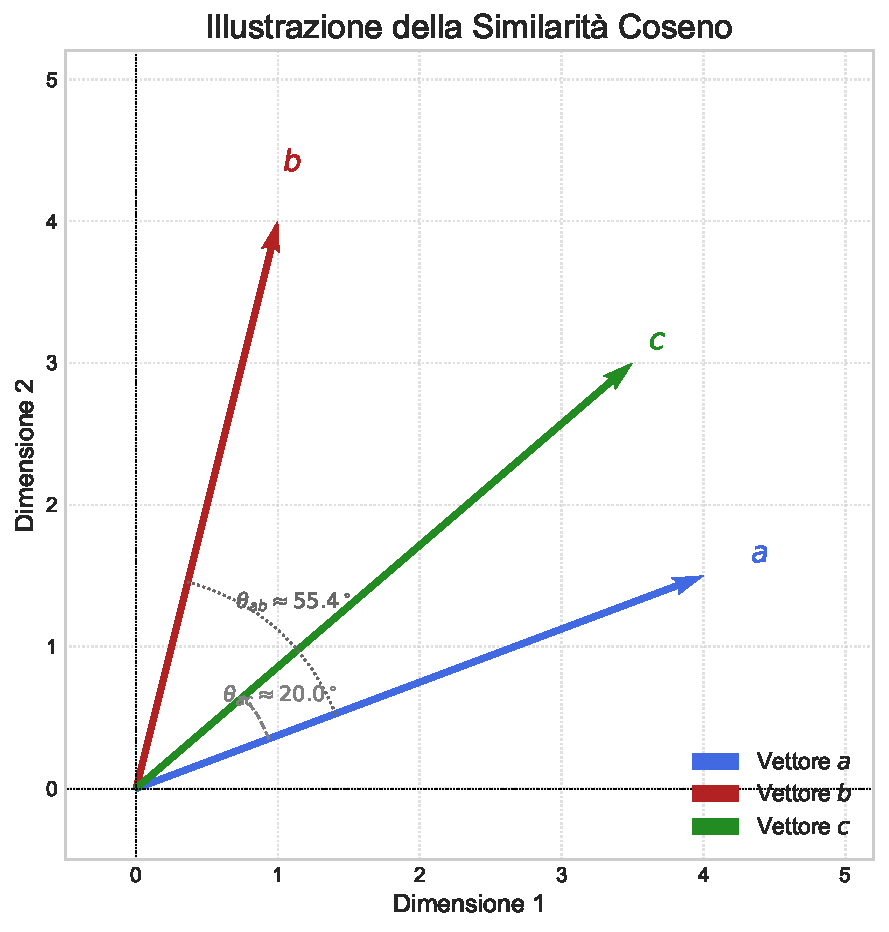
\includegraphics[width=0.5\textwidth]{images/cosine_similarity_diagram.pdf}
    \caption{Illustrazione della similarità coseno: il vettore $a$ è più simile a $c$ che a $b$, poiché l'angolo tra $a$ e $c$ è minore.}
    \label{fig:cosine_similarity_diagram}
\end{figure}

\subsection{Full Text Search (FTS) e Modelli di Information Retrieval}
L'\textbf{Information Retrieval (IR)} si occupa della ricerca di informazioni (tipicamente testuali) all'interno di collezioni di documenti, in risposta a una query dell'utente. La \textbf{Full Text Search (FTS)} è una tecnica fondamentale dell'IR. Richiede l'estrazione e l'indicizzazione dei termini presenti in ogni documento, spesso precedute dalle tecniche di pre-processamento viste.
Se la query contiene più termini, occorre specificare come si combinano (es. devono comparire tutti? devono essere vicini?). Si possono anche voler individuare termini simili (sinonimi) a quelli della query. I documenti recuperati devono essere ordinati per rilevanza.

\subsubsection{Compromesso tra Precision e Recall nella FTS}
La bontà di un sistema FTS viene spesso misurata in termini di:
\begin{itemize}
    \item \textbf{Precision}: Percentuale di documenti rilevanti tra quelli restituiti dal sistema.
          $$ \text{Precision} = \frac{|\{\text{Documenti Rilevanti}\} \cap \{\text{Documenti Restituiti}\}|}{|\{\text{Documenti Restituiti}\}|} $$
    \item \textbf{Recall}: Percentuale di documenti rilevanti restituiti dal sistema tra tutti i documenti rilevanti presenti nella collezione.
          $$ \text{Recall} = \frac{|\{\text{Documenti Rilevanti}\} \cap \{\text{Documenti Restituiti}\}|}{|\{\text{Documenti Rilevanti}\}|} $$
\end{itemize}
Esiste tendenzialmente un trade-off: modificando i parametri di un sistema FTS per migliorare uno dei due aspetti (es. aumentare il numero di documenti restituiti per aumentare la recall), l'altro tende a peggiorare (la precision potrebbe diminuire perché vengono inclusi più documenti non rilevanti).

\subsubsection{Modelli di Information Retrieval}
Sono stati elaborati diversi modelli per rappresentare e recuperare documenti:
\begin{itemize}
    \item \textbf{Classificazione dei Modelli}: Possono essere basati sulla teoria degli insiemi (es. Modello Booleano), sull'algebra (es. Vector Space Model) o sulla probabilità. Possono considerare o meno l'interdipendenza dei termini (ignorata, intrinseca al modello, o definita da fonti esterne).
    \item \textbf{Modello Booleano Standard}:
          \begin{itemize}
              \item I documenti sono considerati rilevanti o non rilevanti rispetto a una query. Quelli rilevanti sono restituiti senza un ordine specifico.
              \item A un termine di ricerca è associato l'insieme dei documenti che lo contengono.
              \item I termini possono essere combinati con operatori logici (AND $\rightarrow$ intersezione insiemi; OR $\rightarrow$ unione insiemi).
              \item \textit{Pro}: Concettualmente semplice, facile da implementare.
              \item \textit{Contro}: Restituisce documenti non ordinati per rilevanza e spesso in quantità troppo alta o troppo bassa (tutto o niente).
          \end{itemize}
    \item \textbf{Vector Space Model (VSM) vs Modello Booleano}:
          \begin{itemize}
              \item Il VSM (con similarità coseno) permette di ottenere un ranking effettivo dei documenti dal più rilevante al meno rilevante.
              \item L'output non è limitato come nel modello booleano; si può porre una soglia di similarità o fissare il numero di risultati.
              \item Il VSM base non supporta direttamente espressioni booleane complesse, ma esistono modelli estesi che combinano VSM e logica booleana (es. recupero booleano seguito da ranking VSM).
          \end{itemize}
    \item \textbf{Modelli con Dipendenze tra Termini}: Alcuni modelli considerano esplicitamente le dipendenze reciproche tra termini (es. sinonimia, correlazioni) per migliorare la ricerca.
          \begin{itemize}
              \item \textit{Dipendenze Intrinseche}: Dedotte statisticamente dalla collezione di documenti (es. Latent Semantic Analysis - LSA, che traspone documenti e query in uno spazio di "concetti semantici" latenti).
              \item \textit{Dipendenze Trascendenti}: Definite da una base di conoscenza esterna (es. un thesaurus o una rete semantica come WordNet).
          \end{itemize}
\end{itemize}

\subsubsection{Ricerca Efficiente: Indicizzazione}
Per recuperare rapidamente i documenti rilevanti per una query da una grande collezione, la ricerca sequenziale (che controlla ogni documento) è troppo lenta ($O(N)$ con $N$ numero di documenti). Si utilizzano quindi strutture dati chiamate \textbf{indici}.
L'\textbf{indice inverso (inverted index)} è una struttura tipica che associa a ogni termine la lista dei documenti in cui compare. Dato un termine, l'accesso alla lista dei documenti è molto rapido (idealmente $O(1)$, come per una HashMap). L'indice viene costruito e mantenuto aggiornato processando la collezione di documenti.

\subsection{Estrarre la Semantica di un Testo}
Le tecniche di pre-processamento e rappresentazione come il BoW sono mirate principalmente alla sintassi e alla struttura superficiale, ottenendo una rappresentazione strutturata ma di basso livello. Per una comprensione più profonda, si applicano tecniche per interpretare il \textbf{significato} (semantica) che il testo vuole comunicare.
Una comprensione completa ed esatta del significato è un problema molto complesso per un calcolatore, spesso affrontato con tecniche che simulano il ragionamento umano (es. deep learning). Tuttavia, per molti compiti (es. capire se due testi trattano lo stesso argomento), una comprensione esatta non è sempre necessaria; può essere sufficiente osservare che le parole più frequenti sono le stesse o semanticamente correlate.

\subsubsection{Basi di Conoscenza Semantiche}
Per interpretare il significato, è necessario conoscere le parole esistenti e le loro relazioni (sinonimia, gerarchie, ecc.). Gli algoritmi di analisi testuale, specialmente quelli semantici, usano spesso basi di conoscenza esterne del linguaggio, costituite da insiemi di parole con diverse informazioni associate.

\paragraph{WordNet.}
WordNet è uno dei più noti database lessicali per la lingua inglese (esistono WordNet anche per altre lingue). Include oltre 150.000 termini (nomi, verbi, aggettivi, avverbi) organizzati in più di 100.000 \textbf{synset} (synonym sets).
\begin{itemize}
    \item Un \textbf{synset} è un insieme di parole (sinonimi) che condividono un significato unico e specifico.
    \item Ogni synset ha una breve descrizione testuale del significato (detta \textbf{gloss}).
    \item Uno stesso termine può essere presente in molteplici synset se è polisemico (ha più significati).
    \item Tra i synset e tra i singoli termini sono definite relazioni semantiche e lessicali.
\end{itemize}
Principali relazioni semantiche in WordNet:
\begin{itemize}
    \item \textbf{Iponimia (is-a)}: Relazione di specificità (es. "cane" è iponimo di "animale"). La relazione opposta è l'\textbf{iperonimia} ("animale" è iperonimo di "cane"). Questa relazione forma una tassonomia gerarchica (ad albero) dei nomi.
    \item \textbf{Meronimia (part-of / member-of / substance-of)}: Indica una relazione parte-tutto (es. "motore" è meronimo di "automobile"). La relazione opposta è l'\textbf{olonimia} (has-a).
    \item \textbf{Implicazione (entailment)}: Un'azione ne comporta un'altra (es. "mangiare" implica "masticare" e "ingoiare").
    \item \textbf{Antonimia}: Indica un significato opposto (relazione lessicale tra parole, es. "uomo" e "donna").
\end{itemize}

\begin{figure}[H]
    \centering
    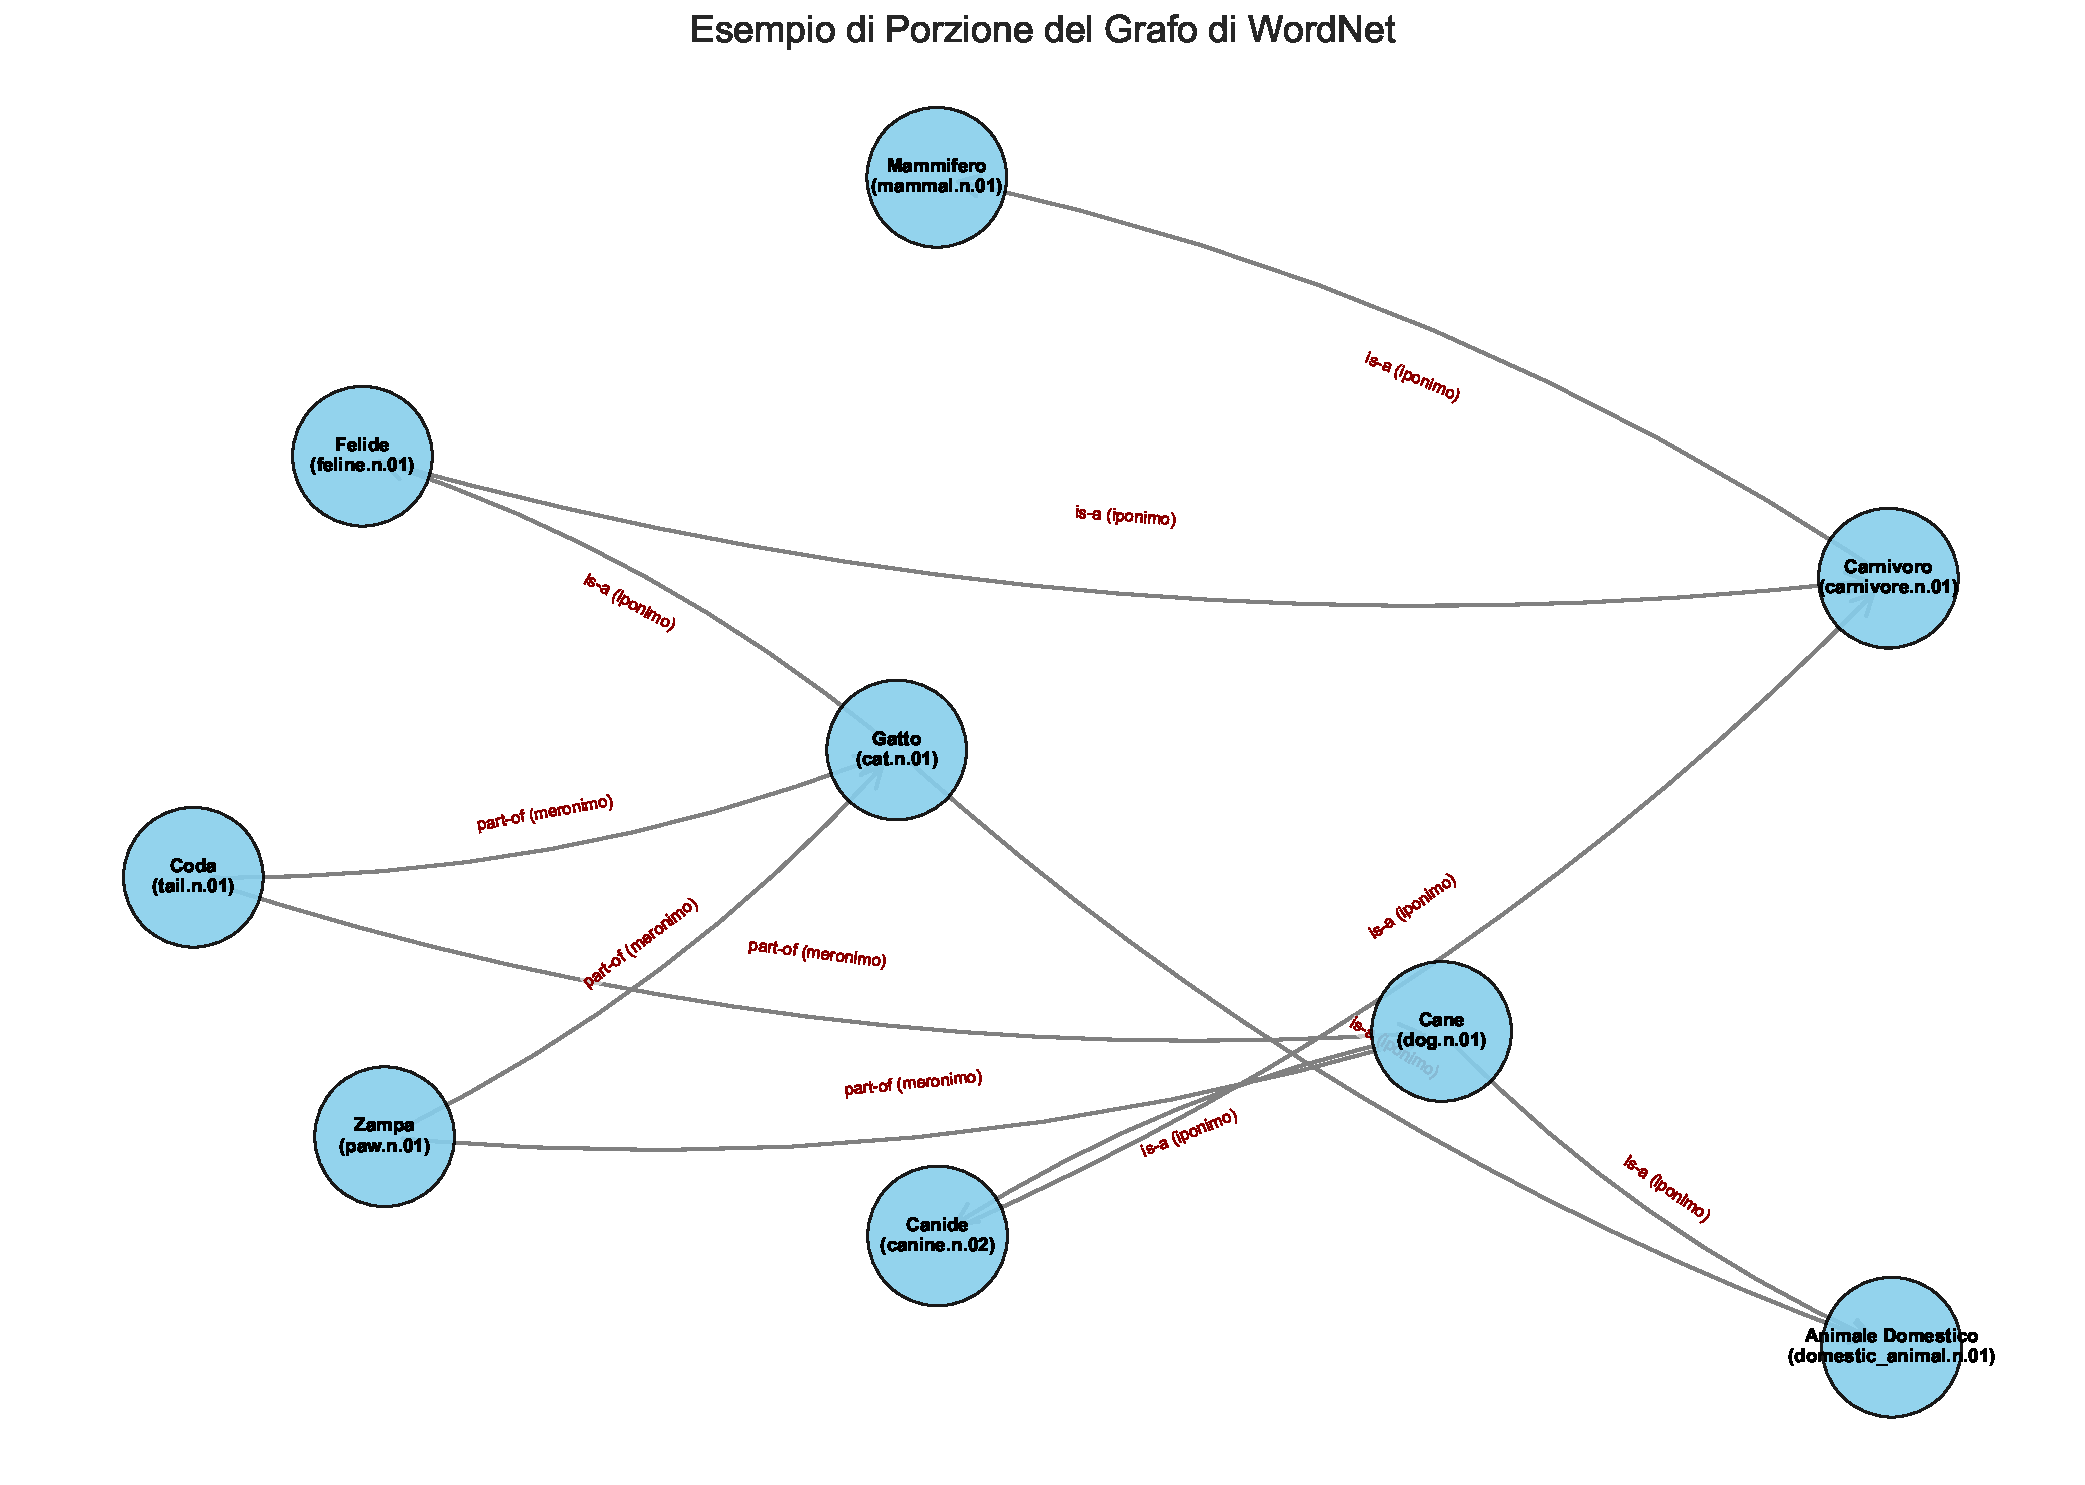
\includegraphics[width=\textwidth]{images/wordnet_graph_example.pdf}
    \caption{Esempio di una porzione del grafo di WordNet, illustrante synset e relazioni semantiche.}
    \label{fig:wordnet_graph}
\end{figure}

\subsubsection{Word Sense Disambiguation (WSD)}
La \textbf{Word Sense Disambiguation (WSD)} è il compito di associare a ogni parola polisemica in un testo il suo significato (senso) esatto nel contesto specifico. Ad esempio, distinguere se la parola "spina" si riferisca a un aculeo, a un connettore elettrico, o altro.
La WSD richiede una base di conoscenza che associ ad ogni parola i suoi possibili significati (es. WordNet). La disambiguazione avviene tipicamente analizzando il \textbf{contesto} della parola, ovvero le parole vicine.
L'\textbf{algoritmo di Lesk} è un approccio classico: per una parola ambigua, si sceglie il senso la cui definizione (gloss nel caso di WordNet) ha il maggior numero di parole in comune con il contesto in cui appare la parola ambigua.

\subsubsection{Named Entity Recognition (NER)}
Una \textbf{named entity} (entità nominata) è un'entità del mondo reale a cui ci si può riferire per nome in un testo, come persone (es. "Presidente Obama"), luoghi (es. "Germania"), organizzazioni (es. "ONU"). A volte sono considerate named entity anche elementi come numeri, date, valute (es. "25 dicembre", "20€"). Le named entity sono spesso tra gli elementi più informativi di un testo.
La \textbf{Named Entity Recognition (NER)} consiste nell'individuare le named entity in un testo e classificarle secondo tipi predefiniti (es. PERSON, LOCATION, ORGANIZATION, MISC, ecc.).

\subsection{Applicazioni NLP: Stima della Customer Satisfaction da Dati Testuali}
Valutare il grado di soddisfazione dei clienti è cruciale, ad esempio in un contesto e-commerce. Le recensioni testuali sono una fonte importante di informazione. Se le recensioni hanno un punteggio numerico esplicito, misurare il gradimento è facile. Altrimenti, o in aggiunta, è utile estrarre informazioni direttamente dal testo scritto (es. da post su forum, social network).

\subsubsection{Metodi Basati su Parole Chiave}
Un metodo semplice per valutare una recensione è verificare la presenza di parole chiave che indicano soddisfazione o insoddisfazione.
\begin{itemize}
    \item Si creano (o si usano) liste predefinite di parole con connotazione positiva (es. "capolavoro", "ottimo", "consigliato") e negativa (es. "orribile", "mediocre", "deludente").
    \item Si contano quante parole di ciascuna lista sono presenti nel testo della recensione.
    \item Confrontando i conteggi, si ottiene una stima del grado di soddisfazione.
\end{itemize}
Limiti di questo approccio:
\begin{itemize}
    \item Le liste sono laboriose da compilare, difficilmente complete e specifiche per lingua e dominio.
    \item Termini specifici possono avere connotazioni diverse a seconda della categoria di prodotto (es. "small" è positivo per una fotocamera, negativo per una stanza d'albergo).
\end{itemize}

\subsubsection{Approccio Basato su Machine Learning}
È possibile estrarre un classificatore da recensioni pre-etichettate (es. come "positive" e "negative") per stimare la polarità di nuove recensioni.
\begin{itemize}
    \item L'algoritmo di classificazione (apprendimento supervisionato) analizza un training set di recensioni etichettate per estrarre un modello di conoscenza.
    \item Per trattare i testi, è necessario rappresentarli come vettori (es. usando il Vector Space Model, con pesi TF o TF-IDF). La presenza/peso di ciascun termine costituisce una feature.
    \item L'algoritmo individua i termini (o combinazioni di termini) con maggiore capacità discriminativa tra le classi.
\end{itemize}
Questo approccio può adattarsi meglio al contesto specifico e alla lingua dei dati rispetto alle liste di parole chiave fisse.

\subsubsection{Utilizzo di Informazione Esterna}
Oltre alle recensioni interne a una piattaforma e-commerce, si possono reperire informazioni e pareri da fonti esterne sul Web (social network, blog, forum specializzati) per valutare meglio la reputazione di un prodotto o servizio. Molti servizi online offrono API (Application Programming Interfaces) per accedere automaticamente a questi dati (es. Twitter API per l'accesso ai tweet).

\begin{notebox}{Limiti e Sfide nell'Analisi del Sentimento}
    Approcci semplici come il conteggio di parole (Bag-of-Words) ignorano l'ordine delle parole e la struttura delle frasi. Questo causa problemi con:
    \begin{itemize}
        \item \textbf{Negazioni}: Frasi come "not bad" possono essere erroneamente giudicate negative per la presenza del termine "bad", ignorando la negazione "not".
        \item \textbf{Sarcasmo e Ironia}: Molto difficili da rilevare automaticamente.
        \item \textbf{Confronti} tra oggetti e \textbf{frasi ipotetiche}.
    \end{itemize}
    Soluzioni più avanzate cercano di affrontare queste limitazioni.
\end{notebox}

\begin{examplebox}{Ricerca Prodotti Medicali}
    Un'azienda che distribuisce prodotti medicali con descrizioni testuali brevi e di bassa qualità (abbreviazioni, termini concatenati, unità di misura nel testo) necessitava di un motore di ricerca per keyword che restituisse prodotti ordinati per rilevanza.
    La soluzione concettuale adottata:
    \begin{enumerate}
        \item Pre-processing spinto del testo (eliminazione simboli, punteggiatura, gestione numeri, ecc.).
        \item Costruzione di Bag-of-Words utilizzando unigrammi e trigrammi per catturare più informazione da testi brevi.
        \item Creazione di una matrice Trigrammi x Prodotti (eventualmente passando da matrici intermedie Trigrammi x Parole e Parole x Prodotti).
        \item Applicazione di TF-IDF.
        \item Rappresentazione della query dell'utente come un vettore di trigrammi (come se fosse un prodotto).
        \item Ricerca dei prodotti più simili alla query utilizzando la similarità coseno (o Jaccard) e una soglia.
    \end{enumerate}
\end{examplebox}

% Fine Aula_introduzione_a_nlp.pdf

\end{document}